\documentclass[12pt,a4paper]{report}
\usepackage[utf8]{inputenc}
\usepackage[czech]{babel}
\usepackage[T1]{fontenc}

% radkovani 1,5, ale ne u footnotes, literatury, ...
% baselinestretch 1.3 je radkovani 1,5
% https://theses.cz/id/say3ul/BP.pdf
% http://mirrors.nic.cz/tex-archive/info/czech/latex-pro-pragmatiky/latex-pro-pragmatiky.pdf
%\renewcommand{\baselinestretch}{1.3}
% To by bylo i v caption apod.
% https://texfaq.org/FAQ-linespace
\usepackage[onehalfspacing]{setspace}

% TODO predepsane okraje
\usepackage[
    a4paper,
    left=40mm,
    right=15mm,
    top=25mm,
    bottom=30mm,
    % includefoot ??
    marginparwidth=35mm,
    marginparsep=3mm,
    %showframe,
]{geometry}
\usepackage{array}
%\usepackage{multirow}
\usepackage{siunitx}
\usepackage{graphicx}
\usepackage{booktabs}
%\usepackage{calc} % e.g. for calculations in desky-predni
%\usepackage{refcount} % calculations with references (Lastpage in desky-predni)
%\usepackage{makecell} % for multiline cells
%\usepackage{lastpage}

%\usepackage{fancyhdr}

\usepackage{titling}
%\usepackage{tabularx}
%\usepackage{colortbl}
%\usepackage{hhline}
\usepackage{float}
\usepackage{csquotes}
\usepackage[backend=biber,style=iso-numeric]{biblatex}
\addbibresource{reference.bib}
\usepackage[czech]{varioref}
\usepackage[unicode,hidelinks]{hyperref}
\usepackage{pdflscape}
\usepackage{amsmath}
%\usepackage{wrapfig}
\usepackage{caption}
\usepackage{subcaption}
\usepackage{catchfile}
\usepackage[
    %section
]{placeins} % provides \FloatBarrier
\usepackage[EFvoltages,siunitx,european, american inductors]{circuitikz}

\usepackage{enumitem}
\usepackage{listings}
\usepackage[htt]{hyphenat}  % hyphenate \texttt
\usepackage{titlesec}
\usepackage{acronym}
\usepackage[titles]{tocloft}
\usepackage[
    %disable
    % todonotes can do weird stuff with circuitikz/tikz node[above], even when
    % disabled
]{todonotes}
\reversemarginpar
\usepackage{dirtree}
\usepackage{pdfpages}

% Typesetting LCD displays with custom characters.
% Full documentation for this package can be build from sources downloaded from
% CTAN.
\usepackage{lcd}
\usepackage{longtable}
\usepackage{csvsimple}

\usetikzlibrary{fit}

%\usepackage{arydshln} % dashed lines in tabular; should be one of the last packages (http://texdoc.net/texmf-dist/doc/latex/arydshln/arydshln-man.pdf)

\graphicspath{{figures/}{sim/}{hodnoty/}} % figures and gnuplot EPS stuff


% TODO patching babel failed
\makeatletter
\newcommand\my@hyphen{-}
\patchcmd\select@language{-}{\my@hyphen }{}{\fail}
\makeatother


% http://www.gnuplotting.org/labels-with-white-background-in-latex-terminals/
\newcommand{\hl}[1]{\setlength{\fboxsep}{0.75pt}\colorbox{white}{#1}}

% robust command because of \listoffigures
\DeclareRobustCommand{\HAentity}[1]{\texttt{\detokenize{#1}}}  % detokenize makes underscores printable
\DeclareRobustCommand{\HAdomain}[1]{\href{https://www.home-assistant.io/integrations/#1/}{\texttt{\detokenize{#1}}}}
\DeclareRobustCommand{\HAintegration}[1]{\href{https://www.home-assistant.io/integrations/#1/}{\texttt{\detokenize{#1}}}}
\DeclareRobustCommand{\shellcmd}[1]{\texttt{\detokenize{#1}}}  % POZOR na '--' ve flags
\newcommand{\HAstate}{\texttt}
\DeclareRobustCommand{\topic}[1]{\texttt{\detokenize{#1}}}
\newcommand{\gitrepo}{\texttt}
\newcommand{\gitbranch}[1]{\texttt{#1}}
\DeclareRobustCommand{\repopath}[1]{\texttt{\detokenize{#1}}}
\newcommand{\filename}{\texttt}
\DeclareRobustCommand{\yamlkey}[1]{\texttt{\detokenize{#1}}}
\DeclareRobustCommand{\inikey}[1]{\texttt{\detokenize{#1}}}
\newcommand{\port}[1]{\texttt{#1}} % TCP/UDP port
\newcommand{\MCUpin}{\texttt}
\newcommand{\IIC}{I\textsuperscript{2}C}
\newcommand{\ipaddress}{\texttt}

\title{Chytrý budík}
\author{Ondřej Sluka}
\date{2022}  % TODO

\frenchspacing
\sisetup{
    output-decimal-marker = {,},
    list-separator = {; },
    list-final-separator = { a~},
    list-pair-separator = { a~},
    group-digits,
    group-minimum-digits=4,
    range-phrase=\text{--},
    range-units=single,
    exponent-product=\ensuremath{\cdot}
}

\DeclareSIUnit{\sample}{Sa}


\makeatletter
\@ifpackageloaded{setspace}{%
    % https://tex.stackexchange.com/questions/55802/latex-lstinline
    \newcommand{\mysinglespacing}{%
      \setstretch{1}% no correction afterwards
    }
}{%
    \newcommand{\mysinglespacing}{}
}
\makeatother


\newcommand{\lstpostbreak}{\mbox{$\hookrightarrow$\space}}

% https://tex.stackexchange.com/questions/30512/how-to-insert-code-with-accents-with-listings
\lstset{
  basicstyle=\mysinglespacing\fontfamily{lmtt}\selectfont,
  columns=flexible,
  breaklines=true,
  postbreak=\lstpostbreak,
  showstringspaces=false,
  literate=%
    {á}{{\'a}}1
    {í}{{\'i}}1
    {é}{{\'e}}1
    {ý}{{\'y}}1
    {ú}{{\'u}}1
    {ó}{{\'o}}1
    {ě}{{\v{e}}}1
    {š}{{\v{s}}}1
    {č}{{\v{c}}}1
    {ř}{{\v{r}}}1
    {ž}{{\v{z}}}1
    {ď}{{\v{d}}}1
    {ť}{{\v{t}}}1
    {ň}{{\v{n}}}1
    {ů}{{\r{u}}}1
    {Á}{{\'A}}1
    {Í}{{\'I}}1
    {É}{{\'E}}1
    {Ý}{{\'Y}}1
    {Ú}{{\'U}}1
    {Ó}{{\'O}}1
    {Ě}{{\v{E}}}1
    {Š}{{\v{S}}}1
    {Č}{{\v{C}}}1
    {Ř}{{\v{R}}}1
    {Ž}{{\v{Z}}}1
    {Ď}{{\v{D}}}1
    {Ť}{{\v{T}}}1
    {Ň}{{\v{N}}}1
    {Ů}{{\r{U}}}1
}
  %literate={█}{{\#}}1

\lstdefinestyle{numbers}{
    numbers=left,
    xleftmargin=2em,
    %framexleftmargin=1.5em,  % cisla radku uvnitr ramecku, vypada hnusne
}

\lstdefinestyle{terminal}{
    basicstyle=\ttfamily\mysinglespacing,
    basewidth={0.5em,0.5em},
    frame=single,
    frameround=tttt,
}


\lstdefinelanguage{Ini}
{
    morecomment=[s][\bfseries]{[}{]},
    morecomment=[l]{\#},
    morecomment=[l]{;},
    morekeywords={},
    literate =%
        {-}{{-}}1
}

\lstdefinelanguage{yaml}
{
    columns=[l]flexible,
    %
    morekeywords={%
        true,false,null,
        !secret,!include,!include_dir_list,!include_dir_named,
        !include_dir_merge_list,!include_dir_merge_named
    },
    alsoletter={!},
    sensitive=false,
    %
    comment=[l]{\#},
    %
    morestring=[d]',
    morestring=[b]",
    %stringstyle=\mdseries\ttfamily\itshape,  % only for testing
    showstringspaces = false,
    % multiline strings >- -- looks too hard to implement
    %
    %moredelim=[l][\color{orange}]{\&},
    %moredelim=[l][\color{magenta}]{*},
    %
    % TODO YAML syntax highlighting - \bfseries keys not compatible with multiline strings
    %basicstyle=\bfseries\mysinglespacing,
    %moredelim=**[il][\mdseries{:}]{:}, % switch to value style at :
    %moredelim=[l][\mdseries]{:}, % switch to value style at :
    %
    % alsolanguage jinja2 -- too complicated
    %
    literate =  {---}{{\llap{\mdseries-{-}-}}}3
                {>}{{\textgreater}}1
                {>-}{{\textgreater-}}2
                {|}{{\textbar}}1
                {|-}{{\textbar-}}2
                % make dashes shorter
                {-}{{-}}1
                {-\ }{{\mdseries-\ }}2,
}

\lstdefinelanguage{Poke}
{
    sensitive=true,
    % see poke.vim in poke 2.1
    morekeywords={%
        % statement
        assert,break,continue,return,
        type,unit,fun,method,
        var,
        % operators
        in,sizeof,as,isa,unmap,
        % conditionals
        if,else,where,
        %
        struct,union,pinned,
        % loops
        while,for,
        % imports
        load,
        try,catch,until,raise,
        % exceptions - skipped
        % types
        string,void,int,uint,bit,nibble,
        byte,char,ushort,short,ulong,long,
        uint8,uint16,uint32,uint64,
        off64,uoff64,offset,
        Comparator,POSIX_Time32,POSIX_Time64,
        big,little,any,
        % constants
        ENDIAN_LITTLE,ENDIAN_BIG,
        IOS_F_READ,IOS_F_WRITE,IOS_F_CREATE,
        IOS_M_RDONLY,IOS_M_WRONLY,IOS_M_RDWR,
        load_path,NULL,OFFSET,
        % Poke std lib
        print,printf,catos,stoca,atoi,ltos,reverse,
        ltrim,rtrim,strchr,qsort,crc32,alignto,
        open,close,flush,get_ios,set_ios,iosize,
        rand,get_endian,set_endian,strace,exit,
        getenv,
        % integer literals - skipped
        % Units
        b,M,B,
        Kb,KB,Mb,MB,Gb,GB,
        Kib,KiB,Mib,MiB,Gib,GiB,
        % offsets - skipped
    },
    morecomment=[s]{/*}{*/},
    morecomment=[l]//,
    morestring=[b]",
    moredelim=[s][keywordstyle]{<}{>}  % uint<x>
}

% https://tex.stackexchange.com/questions/312/correctly-typesetting-a-tilde/160898#160898
\makeatletter
\newcommand\midtilde@raisedtilde[1][.5]{\raisebox{#1ex}{\texttildelow}}
\def\midtilde@normaltilde{\texttildelow}

\newcommand\midtilde%
{%
  \expandafter\in@\expandafter{\f@family}%
    {cmr,cmss,cmtt,cmm,cmsy,cmx,%
    lmr,lmss,lmtt,lmm,lmsy,lmx,%
    pxr,pxss,pxm,pxsy,pxx,%
    txr,txss,txm,txsy,txx}%
  \ifin@%
    \midtilde@raisedtilde%
  \else%
    \expandafter\in@\expandafter{\f@family}%
    {pxtt,txtt}%
    \ifin@%
      \midtilde@raisedtilde[.35]%
    \else%
      \midtilde@normaltilde%
    \fi%
  \fi%
}
\makeatother
\lstdefinelanguage{mybash}
{
    language = bash,
    literate =%
        % $# is not a comment...
        {\$\#}{{{\$\#}}}2 {\$\# }{{{\$\# }}}2
        % make dashes shorter
        {-}{{-}}1
        {~}{{\midtilde}}1
        % komentare s diakritikou
        {á}{{\'a}}1
        {í}{{\'i}}1
        {é}{{\'e}}1
        {ý}{{\'y}}1
        {ú}{{\'u}}1
        {ó}{{\'o}}1
        {ě}{{\v{e}}}1
        {š}{{\v{s}}}1
        {č}{{\v{c}}}1
        {ř}{{\v{r}}}1
        {ž}{{\v{z}}}1
        {ď}{{\v{d}}}1
        {ť}{{\v{t}}}1
        {ň}{{\v{n}}}1
        {ů}{{\r{u}}}1
        {Á}{{\'A}}1
        {Í}{{\'I}}1
        {É}{{\'E}}1
        {Ý}{{\'Y}}1
        {Ú}{{\'U}}1
        {Ó}{{\'O}}1
        {Ě}{{\v{E}}}1
        {Š}{{\v{S}}}1
        {Č}{{\v{C}}}1
        {Ř}{{\v{R}}}1
        {Ž}{{\v{Z}}}1
        {Ď}{{\v{D}}}1
        {Ť}{{\v{T}}}1
        {Ň}{{\v{N}}}1
        {Ů}{{\r{U}}}1
}

\lstdefinelanguage{Dockerfile}{
    keywords={FROM, RUN, COPY, ADD, ENTRYPOINT, CMD,  ENV, ARG, WORKDIR, EXPOSE, LABEL, USER, VOLUME, STOPSIGNAL, ONBUILD, MAINTAINER},
    sensitive=false,
    comment=[l]{\#},
    morestring=[b]',
    morestring=[b]",
    literate =%
        {-}{{-}}1
}

\lstdefinelanguage{myC++}{
    language=C++,
    morekeywords={%
        uint8_t, uint16_t, uint32_t,
        int8_t, int16_t, int32_t,
        size_t,
        constexpr,
        byte
    }
}

\lstdefinelanguage{hashcomment}{
    comment=[l]{\#},
}



% fancyhdr does not seem to work well with documentclass report
% headers and footers
%\setlength{\headheight}{15pt} % prevents a warning most likely caused by diacritics
%\pagestyle{fancy}
%%\renewcommand{\headrulewidth}{0pt}
%\fancyhf{} % clears header and footer, otherwise "plain" will appear
%%\fancyhead{} % only clears the header
%\lhead{\theauthor}
%\rhead{\thepage}
%\fancyhfoffset{0pt} % fixes width after \newgeometry

% Roztrhana matika
\allowdisplaybreaks

% kapitola bez cisla
\newcommand{\nonuchapter}[1]
{%
    \chapter*{#1}%
    \addcontentsline{toc}{chapter}{#1}% v toc, ale bez cisla
    \phantomsection%
}

% seznam priloh
% https://tex.stackexchange.com/questions/26732/how-to-get-a-list-of-appendices
\newcommand{\listappendicesname}{Seznam příloh}
\newlistof{appendices}{apc}{\listappendicesname}
\renewcommand{\theappendices}{\Alph{appendices}}
\newcommand{\newappendix}[1]{%
    \refstepcounter{appendices}
    \section*{Příloha \theappendices: #1}
    \phantomsection
    \addcontentsline{apc}{appendices}{\protect\numberline{\theappendices}#1}
}

% This file was automatically generated by ./script/LCDchars from prilohy/AlarmClock/lib/GUI/LCDchars.cpp.

\DefineLCDchar{home}{%
    00100%
    01110%
    11111%
    10001%
    10001%
    10001%
    11111%
    00000%
}

\DefineLCDchar{bell}{%
    00100%
    01110%
    01110%
    01110%
    01110%
    11111%
    00000%
    00100%
}

\DefineLCDchar{timer}{%
    11111%
    01110%
    00100%
    00100%
    01110%
    11111%
    00000%
    00000%
}

\DefineLCDchar{apply}{%
    00000%
    00000%
    00001%
    00010%
    10100%
    01000%
    00000%
    00000%
}

\DefineLCDchar{cancel}{%
    00000%
    10001%
    01010%
    00100%
    01010%
    10001%
    00000%
    00000%
}



\begin{document}
\begin{titlepage}
    \begin{center}
        \begin{minipage}[c]{0.18\textwidth}
            
\includegraphics[width=\linewidth]{spse-logo}
        \end{minipage}
        \hfill
        \begin{minipage}[c]{0.8\textwidth}
            \centering
            \bfseries
            \large
            \noindent
            Vyšší odborná škola \\
            a~Střední průmyslová škola elektrotechnická \\
            Plzeň, Koterovská 85
        \end{minipage}

        \vfill

        {\LARGE\bfseries\textsc{Dlouhodobá maturitní práce s~obhajobou}}
    \end{center}
    \vfill
    \noindent
    {\Large Téma: \textbf{\thetitle}}
    \vfill
    {%
        \bfseries
        \noindent
        \begin{tabular}{@{}ll@{}}
            Autor práce:    & \theauthor \\
            Třída:          & 4.O \\
            Vedoucí práce:  & Ing. Karel Hajžman\\
            Dne:            & \thedate
        \end{tabular}

        \vspace*{1cm}
        \noindent
        Hodnocení:
    }
\end{titlepage}

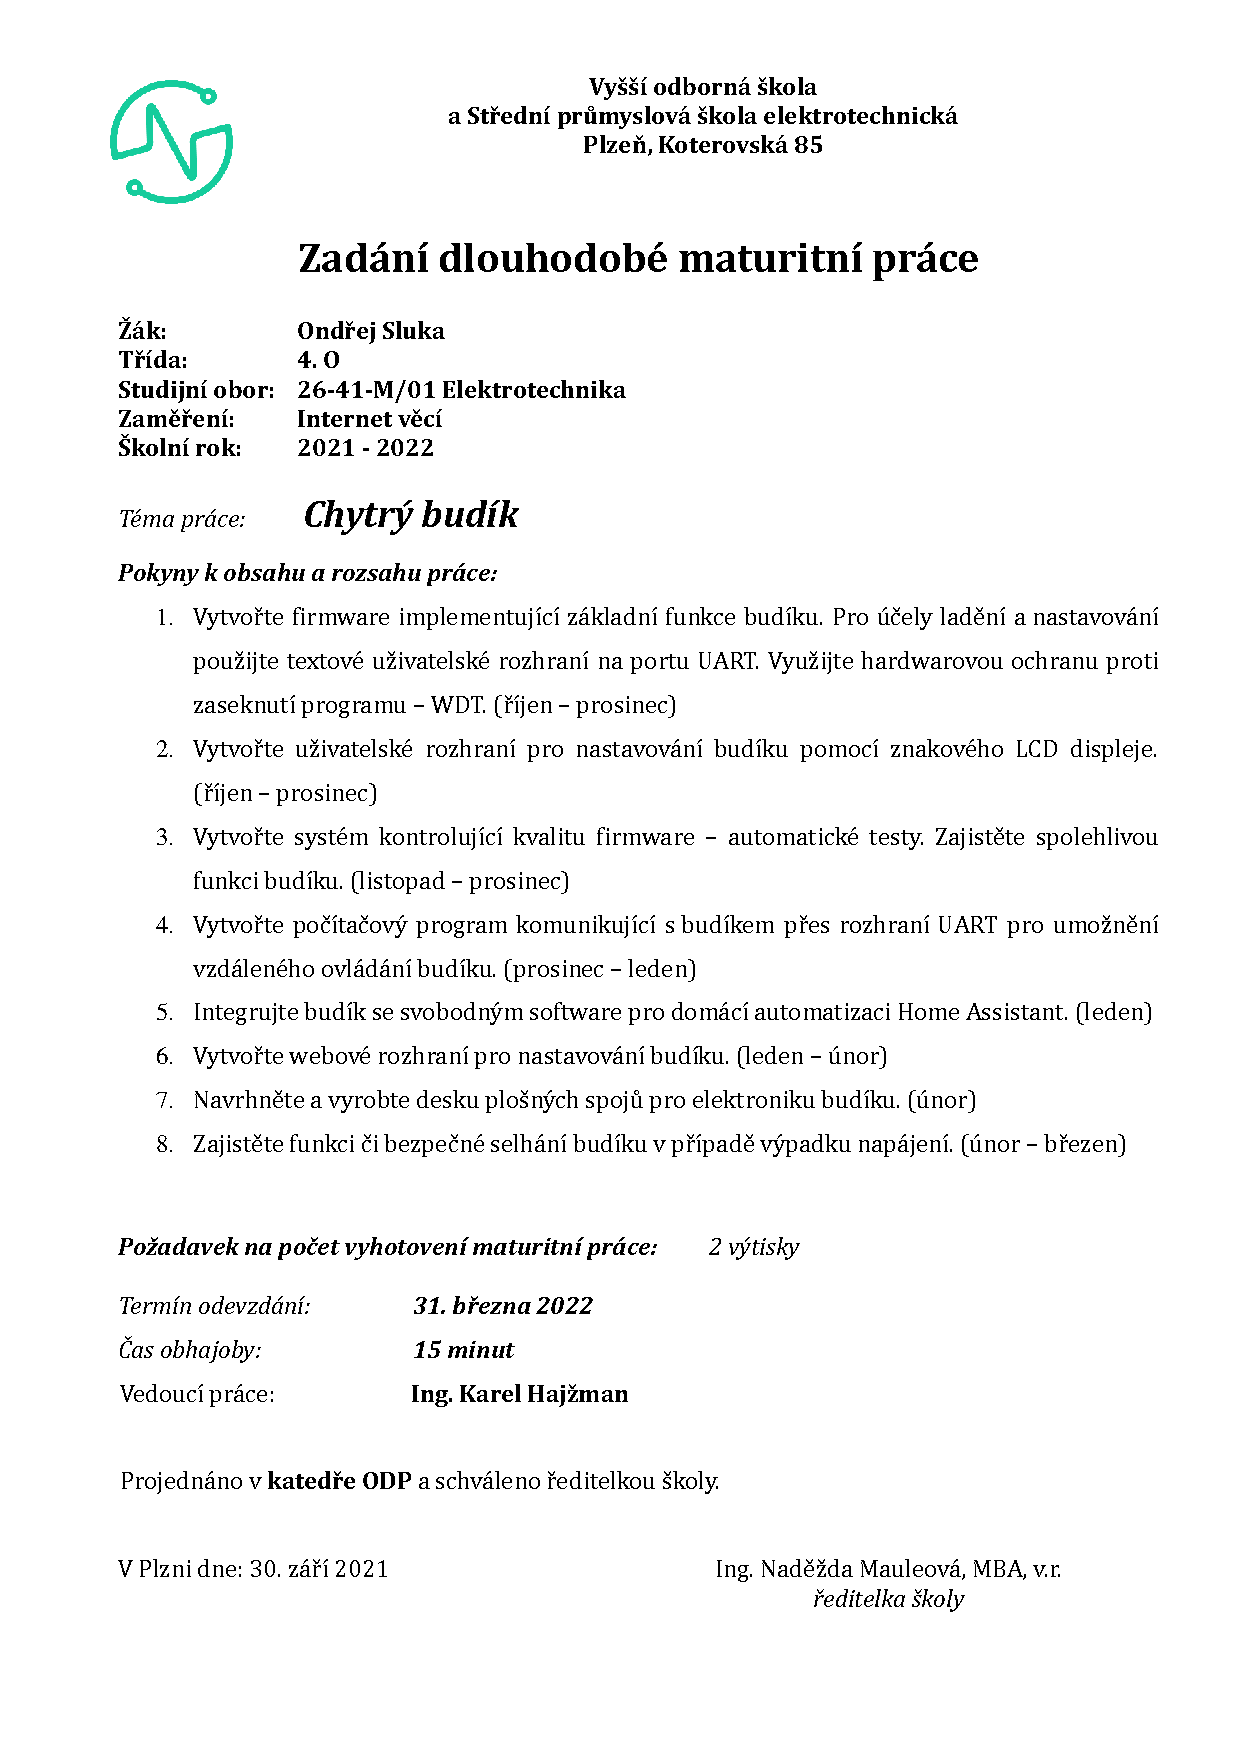
\includepdf{zadani.pdf}
\clearpage
Tato práce se zabývá návrhem a výrobou elektronického budíku s pokročilou
konfigurací. Zařízení lze připojit k serveru s operačním systémem GNU/Linux
s příslušným software a tím dále rozšířit možnosti jeho využití.
\todo[inline]{anotace}

\todo[inline]{podekovani}

\vfill
\noindent
Prohlašuji, že jsem tuto práci vypracoval samostatně a použil literárních
pramenů a~informací, které cituji a uvádím v seznamu použité literatury
a~zdrojů informací.

\noindent
Souhlasím s využitím mé práce učiteli VOŠ a SPŠE Plzeň k výuce.

{%
    \raggedright
    \hfill V~Plzni dne: \dotfill \hspace*{1em}Podpis: \dotfill
    \todo{\texttt{\textbackslash{}dotfill} dava tecky moc vysoko}
}


\tableofcontents

\todo[inline]{monospace v listings -- bold ttfamily}

\nonuchapter{Úvod}
Cílem tohoto projektu je vytvořit budík s pokročilými funkcemi, který lze
snadno vyrobit v amatérských podmínkách a přizpůsobit tak, aby vyhovoval
i požadavkům náročného uživatele--programátora. % TODO

Cílem není vytvořit zařízení přímo připojené k síti Internet. Vzhledem
k charakteru zařízení a skutečnosti, že bude umístěné poblíž hlavy uživatele
po několik hodin denně nepovažuje autor této práce za vhodné využití
bezdrátového přenosu informací. Alternativou by byla technologie Ethernet.
Výhody takového řešení oproti připojení k počítači rozhraním UART ale nejsou
příliš velké a nutnost obsluhovat síťové funkce ve firmware mikrokontroléru by
výrazně omezila možnosti implementace dalších funkcionalit (například zvukového
výstupu).

Dokumentace zdrojového kódu firmware je generována z komentářů pomocí
svobodného nástroje s otevřeným zdrojovým kódem \shellcmd{doxygen}. To
usnadňuje orientaci v projektu a tím umožňuje, aby si i běžný uživatel se
základní znalostí programování implementoval dodatečné funkce, které potřebuje.

TODO vse free
software\footnote{\url{https://www.gnu.org/philosophy/free-sw.html}}.

Mnoho požadavků vychází ze zkušeností s komerčně dostupnými řešeními. Autor
této práce po několik let používal radiobudík Sencor SRC~330~GN.
% TODO obrazek sencor budik
Během používání bylo odhaleno několik problému, především nedostatek
nastavitelných časů buzení (pouze 2), nemožnost přiřadit budicímu času
libovolnou skupinu dní v týdnu a problémy se zrušením budíku v průběhu odložení
funkcí snooze. Nepříjemná byla také chyba ve firmware, která se
projevovala pískáním, které šlo zrušit pouze odpojením napájení budíku,
ke kterému docházelo náhodně v první hodině po stisku tlačítka nastavujícího
dobu nečinnosti, po které dojde ke zhasnutí displeje. Protože tento komerčně
dostupný budík neumožňuje zásah uživatele do firmware, neexistuje žádná
možnost, jak tyto nedostatky odstranit. Mezi další problémy patřilo
i slyšitelné bzučení o frekvenci \SI{50}{\hertz} vydávané interním
transformátorem (zařízení je napájené síťovým napětím).

\chapter{Hardware a firmware}
\subsection{Mikrokontrolér}
Volba MCU byla ovlivněna především autorovými předchozími zkušenostmi
s architekturou 8-bit AVR. Mikrokontroléry ATmega jsou navíc kompatibilní
s platformou Arduino\footnote{\url{https://www.arduino.cc/}}, která umožňuje
jednoduchý vývoj firmware v jazyce C++ bez nutnosti znát všechna specifika
daného MCU. To je v souladu s cíli projektu -- technicky zdatnější uživatel si
může snadno upravit firmware pro své potřeby.

Kromě rozšířenosti v amatérských projektech a dostupnosti vývojových desek ale
zvolený čip ATmega328P nevyniká počtem I/O pinů, výpočetním výkonem,
periferiemi ani cenou. Výhodou je ale jeho dostupnost nejen v pouzdrech pro
povrchovou montáž, ale i v pouzdře s vývody. Použití SMD součástky je totiž na
amatérsky vyrobeném plošném spoji složitější, obzvlášť pokud jde o plošný spoj
jednostranný.

\nocite{dshATmega328} % TODO info o MCU

\section{PlatformIO}
PlatformIO\footnote{\url{https://platformio.org/}} je multiplatformní, na
architektuře nezávislý nástroj s otevřeným zdrojovým kódem pro vývoj embedded
systémů. Podporuje mnoho \acs{SDK} (včetně Arduino) a nezávisí na konkrétním
vývojovém prostředí (\acs{IDE}). Oproti Arduino IDE nabízí možnost pracovat
s příkazovým řádkem namísto grafického rozhraní a díky tomu usnadňuje
automatizaci různých repetitivních procesů ve vývoji firmware. Konfigurační
soubor \filename{platformio.ini} také umožňuje nastavit všechny parametry
sestavení, včetně přímého předávání přepínačů kompilátoru \shellcmd{gcc}.
Je možné vytvořit projekt, který je kompatibilní s Arduino IDE i s PlatformIO,
ale to pouze ztěžuje využívání pokročilých funkcí PlatformIO a nepřináší žádné
výhody.

Nespornou výhodou PlatformIO je správa závislostí~-- knihoven, bez kterých
není možné firmware zkompilovat. Tím, že program v konfiguračním souboru
\filename{platformio.ini} zaznamenává jejich přesné verze, odstraňuje potřebu
vytvářet tuto dokumentaci ručně. Znalost verzí knihoven, se kterými byl
firmware testován, je kritická pro budoucí sestavování. Může se totiž stát, že
v knihovně dojde v novější verzi ke změně API či zanesení chyby. Přístup
Arduino IDE (knihovny sdílené mezi projekty, notifikace doporučující
aktualizaci kdykoli je dostupná novější verze) není pro složitější projekty
závisející na mnoha knihovnách vhodný.

Ukázka obsahu konfiguračního souboru \filename{platformio.ini}:
\begin{lstlisting}[language=Ini]
; PlatformIO Project Configuration File
;
;   Build options: build flags, source filter
;   Upload options: custom upload port, speed and extra flags
;   Library options: dependencies, extra library storages
;   Advanced options: extra scripting
;
; Please visit documentation for the other options and examples
; https://docs.platformio.org/page/projectconf.html

[platformio]
src_dir = AlarmClock

[env:uno]
platform = atmelavr
board = uno
framework = arduino
lib_deps = 
	adafruit/RTClib@^2.0.2
	thomasfredericks/Bounce2@^2.70.0
	paulstoffregen/Encoder@^1.4.1
	marcoschwartz/LiquidCrystal_I2C@^1.1.4
	paulstoffregen/TimerOne@^1.1.0
\end{lstlisting}
Skutečný konfigurační soubor je složitější, protože obsahuje i nastavení
jednotkových testů a různé další úpravy.

Práce s nástrojem pro příkazový řádek PlatformIO Core (CLI) je velmi
jednoduchá. Zkompilování firmware se provádí příkazem
\verb|pio run --environment uno|. Přepínač \verb|--environment| určuje,
pro jakou platformu se má firmware zkompilovat. Lze použít jeho krátkou verzi
\verb|-e|. Výsledný soubor ve formátu Intel HEX se poté nachází v umístění
\repopath{.pio/build/uno/firmware.hex}. Smazání všech zkompilovaných souborů
(užitečné pro vynucení úplného překompilování) se provádí příkazem
\verb|pio run -e uno -t clean|, kde \verb|-t| je krátká verze přepínače
\verb|--target|. Nahrání firmware do mikrokontroléru provádíme příkazem
\verb|pio run -e uno -t upload|.

Pro další zjednodušení a automatizaci práce s tímto nástrojem byl vytvořen
\filename{Makefile}, tedy soubor s pravidly programu GNU \shellcmd{make}.
Tento soubor obsahuje i mechanismus pro generování nápovědy, dostupné příkazy
lze zjistit příkazem \shellcmd{make help}.

\subsection{Automatické testy}
Jednou z hlavních motivací pro nasazení technologie PlatformIO byla podpora
automatických testů. PlatformIO podporuje testování jednotlivých jednotek
zdrojového kódu \foreignlanguage{english}{(unit testing)}, % () uvnitr {}, jinak byla za ( mezera
a to jak na cílové platformě (embedded MCU), tak i na počítači použitém pro
vývoj (native). Testy jsou umístěny v samostatných podsložkách v adresáři
\repopath{test/}.

Pro demonstraci využití jednotkových testů je vhodná velmi jednoduchá jednotka
zajišťující ukládání boolean hodnoty (jednoho bitu, pravda či nepravda) pro
každý den v týdnu -- třída \texttt{DaysOfWeek}. Celý stav tohoto objektu je
reprezentován jedním osmibitovým číslem. Protože je toto číslo přenášeno
rozhraním UART z mikrokontroléru k připojenému počítači, je potřeba zajistit,
že obě strany ukládají hodnoty stejným způsobem. Manuální testování při prvotní
implementaci není dostatečné, protože potřebujeme zabránit možnosti náhodného
neúmyslného poškození funkcionality při pozdějších úpravách kódu. Spouštění
automatických testů při každé změně zdrojového kódu totiž zabírá
několikanásobně méně času než manuální testování. Automatické testy navíc
odstraňují možnost lidské chyby v procesu testování.

Pro pochopení konceptu jednotkových testů nepotřebujeme znát vnitřní
implementaci třídy \texttt{DaysOfWeek} a postačí nám pouhé deklarace jejích
metod z hlavičkového souboru:
\begin{lstlisting}[language=myC++]
#include <stdint.h>

class DaysOfWeek
{
public:
    uint8_t days_of_week = 0x00;
    bool getDayOfWeek(uint8_t num) const;
    bool setDayOfWeek(uint8_t num, bool status);
};
\end{lstlisting}

Kód testu umístíme do souboru
\repopath{test/test_DaysOfWeek/test_DaysOfWeek.cpp}. Připravíme si několik
případů, pro které chceme chování jednotky testovat. Není nezbytně nutné
otestovat všechny možné stavy, často to ani není prakticky možné. Obvykle
postačí několik běžných stavů a případy, které jsou nějakým způsobem speciální
a je u nich proto větší riziko chyby.
\begin{lstlisting}[language=myC++,style=numbers,breakatwhitespace=true]
#include <unity.h>  // unit testing framework
#include <stdint.h>
#include <DaysOfWeek.h>  // testovaná jednotka


struct DowTestCase
{
    uint8_t code;
    bool days[7];
};

// Pole testovaných případů:
DowTestCase Cases[] = {
    {0x00, {false,  false,  false,  false,  false,  false,  false}},
    {0x01, {false,  false,  false,  false,  false,  false,  false}},
    {0x02, {true,   false,  false,  false,  false,  false,  false}},
    // ...
    {0xFE, {true,   true,   true,   true,   true,   true,   true}}
};


// Test dekódování 8bitového čísla code na jednotlivé dny v týdnu:
void test_decode()
{
    // Pro každý testovaný případ...
    for (size_t i = 0; i < sizeof(Cases)/sizeof(Cases[0]); i++)
    {
        // ...vytvoříme nový objekt DaysOfWeek z daného code.
        DaysOfWeek dow(Cases[i].code);
        // V rámci daného případu iterujeme
        // přes všechny dny v týdnu...
        for (size_t j = 0; j < sizeof(Cases[i].days)/sizeof(Cases[i].days[0]); j++)
        {
            // ...a porovnáváme správnou hodnotu daného dne
            // s hodnotou získanou z objektu dow.
            if (Cases[i].days[j])
            {
                TEST_ASSERT_TRUE(dow.getDayOfWeek(j+1));
            }
            else
            {
                TEST_ASSERT_FALSE(dow.getDayOfWeek(j+1));
            }
        }
    }
}


// Test kódování jednotlivých dnů v týdnu do 8bitového čísla:
void test_encode()
{
    // Pro každý testovaný případ...
    for (size_t i = 0; i < sizeof(Cases)/sizeof(Cases[0]); i++)
    {
        // Ošetříme zvláštní případ, který souvisí s faktem,
        // že nejméně významný bit (LSB) je nepoužitý
        // a vždy nulový.
        uint8_t code = Cases[i].code;
        if (code == 0x01) code = 0x00;
        // ...vytvoříme nový objekt DaysOfWeek...
        DaysOfWeek dow;
        // ...a natavíme mu hodnoty jednotlivých dnů v týdnu.
        for (size_t j = 0; j < sizeof(Cases[i].days)/sizeof(Cases[i].days[0]); j++)
        {
            dow.setDayOfWeek(j+1, Cases[i].days[j]);
        }
        // Zkontrojume, zda se 8bitové číslo specifikované
        // testovaným případem shoduje s číslem vytvořeným
        // naším objektem.
        TEST_ASSERT_EQUAL_INT(code, dow.days_of_week);
    }
}


int main(int argc, char **argv)
{
    UNITY_BEGIN();
    // Spustíme výše definované testy.
    RUN_TEST(test_decode);
    RUN_TEST(test_encode);
    UNITY_END();

    return 0;
}
\end{lstlisting}

Spuštění testů provádíme příkazem \shellcmd{pio test}. PlatformIO testovací
program automaticky zkompiluje, nahraje do mikrokontroléru a přes UART přečte
výsledky testů.
% -f test_DaysOfWeek, aby nespoustel ostatni testy
% fixed columns, aby byly zarovnane vysledky
% delka #### progress baru upravena, aby vysly na jeden radek
\begin{lstlisting}[style=terminal,columns=fixed]
$ pio test -e uno
Verbose mode can be enabled via `-v, --verbose` option
Collected 2 items

Processing test_DaysOfWeek in uno environment
-------------------------------------------------------------------
Building...
Uploading...

Warning! Please install `99-platformio-udev.rules`. 
More details: https://docs.platformio.org/page/faq.html#platformio-udev-rules


avrdude: AVR device initialized and ready to accept instructions

Reading | ############################################ | 100% 0.00s

avrdude: Device signature = 0x1e950f (probably m328p)
avrdude: reading input file ".pio/build/uno/firmware.hex"
avrdude: writing flash (3600 bytes):

Writing | ############################################ | 100% 0.60s

avrdude: 3600 bytes of flash written
avrdude: verifying flash memory against .pio/build/uno/firmware.hex:
avrdude: load data flash data from input file .pio/build/uno/firmware.hex:
avrdude: input file .pio/build/uno/firmware.hex contains 3600 bytes
avrdude: reading on-chip flash data:

Reading | ############################################ | 100% 0.47s

avrdude: verifying ...
avrdude: 3600 bytes of flash verified

avrdude: safemode: Fuses OK (E:00, H:00, L:00)

avrdude done.  Thank you.

Testing...
If you don't see any output for the first 10 secs, please reset board (press reset button)

test/test_DaysOfWeek/test_DaysOfWeek.cpp:70:test_decode	[PASSED]
test/test_DaysOfWeek/test_DaysOfWeek.cpp:71:test_encode	[PASSED]
-----------------------
2 Tests 0 Failures 0 Ignored
=================== [PASSED] Took 6.00 seconds ===================

Test             Environment    Status    Duration
---------------  -------------  --------  ------------
test_DaysOfWeek  uno            PASSED    00:00:06.002
=================== 1 succeeded in 00:00:06.002 ===================
\end{lstlisting}

Protože jednotka \texttt{DaysOfWeek} nezávisí na funkcích specifických pro
mikrokontrolér, lze tento test spouštět i v prostředí \texttt{native}, tedy
přímo na PC, na kterém se používá PlatformIO:
\begin{lstlisting}[style=terminal,columns=fixed]
$ pio test -e native
Verbose mode can be enabled via `-v, --verbose` option
Collected 2 items

Processing test_DaysOfWeek in native environment
----------------------------------------------------------------
Building...
Testing...
test/test_DaysOfWeek/test_DaysOfWeek.cpp:70:test_decode	[PASSED]
test/test_DaysOfWeek/test_DaysOfWeek.cpp:71:test_encode	[PASSED]

-----------------------
2 Tests 0 Failures 0 Ignored
OK
================== [PASSED] Took 0.42 seconds ==================

Test             Environment    Status    Duration
---------------  -------------  --------  ------------
test_DaysOfWeek  native         PASSED    00:00:00.419
================= 1 succeeded in 00:00:00.419 =================
\end{lstlisting}

V software poslouchajícím na druhé straně komunikačního rozhraní UART jsou
využitý podobné testy, tentokrát v programovacím jazyce Python, které
kontrolují stejné případy v tamní implementaci objektu. Tím je zajištěna
konzistence mezi firmware a software.


\subsubsection{Pomocné objekty -- mock objects}
Pro testování složitějších jednotek odděleně od ostatních lze využít pomocné
objekty. Při testování firmware je například velmi výhodné takto nahradit kód
komunikující s hardware, protože poté lze testy spouštět i v prostředí
\texttt{native}, naprosto odděleně od vlastního hardware.

Knihovna
\texttt{ArduinoFake}\footnote{\url{https://github.com/FabioBatSilva/ArduinoFake}}
nahrazuje knihovnu \texttt{Arduino.h} a poskytuje definice specifické pro
framework Arduino. Knihovna \texttt{FakeIt}, na které \texttt{ArduinoFake}
staví, umožňuje nahrazovat libovolné metody objektů či funkce vlastní definicí,
díky čemuž je testovaná jednotka zbavena závislostí na ostatních jednotkách.

Jako jednoduchá ukázka poslouží nahrazení funkce \texttt{digitalWrite} sloužící
k ovládání digitálních výstupních pinů:
\begin{lstlisting}[language=myC++]
#include <unity.h>
#include <ArduinoFake.h>
using namespace fakeit;

#include <TestedUnit.h>  // testovaná jednotka závsisející na Arduino.h

void test_example()
{
    // Nastavíme, že funkce digitalWrite po zavolání nic nevrací.
    When(Method(ArduinoFake(), digitalWrite)).AlwaysReturn();

    constexpr uint8_t pin = 1;
    tested_unit.tested_method(pin);  // testovaná funkce

    // Ověříme, zda byla funkce digitalWrite zavolána pouze jednou,
    // a to s prvním argumentem rovným 1 (pin)
    // a druhým argumentem LOW (konstanta definovaná v Arduino.h).
    Verify(Method(ArduinoFake(), digitalWrite).Using(pin, LOW)).Once();
}

// ...
\end{lstlisting}


\subsection{Statická analýza kódu}
Statická analýza kódu umožňuje automaticky detekovat potenciální chyby ve
zdrojovém kódu programu bez jeho spuštění. Program provádějící statickou
analýzu čte zdrojové kódy a odhaluje chyby jako indexování pole mimo jeho
hranice, dereference nulového ukazatele, neinicializovaná proměnná a podobné.

PlatformIO umožňuje využít více různých nástrojů pro statickou analýzu, přičemž
pro jejich obsluhu zavádí příkaz \shellcmd{pio check}. Snadno použitelný
nástroj je \shellcmd{cppcheck}, kterému se proto budeme dále věnovat.

Základní nastavení je velmi jednoduché. Provádí se přidáním záznamu do souboru
\filename{platformio.ini}:
\begin{lstlisting}[language=Ini]
[env:uno]
# ...
check_tool = cppcheck
check_skip_packages = true
check_flags = 
	cppcheck: --suppress=unusedFunction --inline-suppr
check_patterns = 
	AlarmClock/
	lib/
	test/
\end{lstlisting}
Volba \inikey{check_skip_packages} určuje, zda se mají při analýze přeskočit
balíčky třetích stran, jako například framework Arduino. Při jejich
kontrole totiž může dojít vlivem nedokonalosti nástroje \shellcmd{cppcheck}
a jeho nekompatibility s atributem \lstinline[language={[GNU]C++}]!__asm__!
(s částmi kódu v jazyce symbolických adres) k selhání.

Volba \inikey{check_flags} specifikuje přepínače, které se mají nástroji
\shellcmd{cppcheck} předat při jeho spuštění. Příkladem takového přepínače je
\verb|--suppress=unusedFunction|, který potlačí všechna varování týkající se
funkcí, které jsou definovány, ale nejsou využity.

Nástroj není neomylný a v některých případech dojde k falešné detekci. Přepínač
\verb|--inline-suppr| umožňuje potlačení varování pomocí speciálně
formátovaných komentářů přímo v analyzovaném zdrojovém kódu. Bližší informace
o formátu těchto speciálních komentářů lze nalézt v manuálu nástroje
\shellcmd{cppcheck}
v~sekci \foreignlanguage{english}{Inline suppressions}~\cite{cppcheckmanual}.
Příklad jejich využití lze nalézt přímo ve firmware budíku.
V souboru \repopath{lib/SerialCLI/SerialCLI.h} je definováno pole
\lstinline[language=C]!char Serial_buffer_[kSerial_buffer_length_ + 1];!,
které je využíváno pro ukládání neúplného vstupu od uživatele. Vnitřní
implementace třídy \texttt{SerialCLI} nevyžaduje, aby bylo toto pole po celou
dobu životnosti objektu inicializované a obsahovalo validní data (například
nulový znak \lstinline[language=C]!'\0'! v prvním prvku pole).
\shellcmd{cppcheck} ale generuje generuje varování
\begin{lstlisting}[style=terminal,breakatwhitespace=true]
lib/SerialCLI/SerialCLI.h:55: [medium:warning] Member variable 'SerialCLI::Serial_buffer_' is not initialized in the constructor. [uninitMemberVar]
\end{lstlisting}
Řešením by mohlo být pole inicializovat (v hlavičkovém souboru či v
konstruktoru), varování lze ale potlačit i komentářem umístěným nad definici
konstruktoru:
\begin{lstlisting}[language=myC++]
class SerialCLI
{
public:
    // ...

    // cppcheck-suppress uninitMemberVar symbolName=SerialCLI::Serial_buffer_
    SerialCLI(Stream& ser, const command_t* commands,
              const byte command_count,
              void (&print_error)(error_t),
              void (&cmd_not_found)(), const char* prompt
             ) : ser_(ser), commands_(commands),
                 command_count_(command_count),
                 print_error_(print_error),
                 cmd_not_found_(cmd_not_found),
                 prompt_(prompt) { }
\end{lstlisting}

% https://docs.platformio.org/en/latest/plus/pio-check.html

Díky nasazení statické analýzy kódu bylo ve firmware budíku odhaleno několik
potenciálních chyb (čtení z neinicializované proměnné apod.) a stylistických
chyb či nedostatků. Mnoho konstruktorů s jedním parametrem bylo deklarováno bez
klíčového slova \lstinline[language=C++]!explicit!. To mohlo vést ke vzniku
chyb kvůli nezamýšleným implicitním konverzím. Použití
\lstinline[language=C++]!explicit! je vyžadováno například standardem
MISRA C++~\cite[pravidlo 12-1-3]{MISRAC++2008}

Příkladem detekované neinicializované proměnné je
\lstinline[language=C++]!PWMDimmer::value_!. Ta je definována v hlavičkovém
souboru \repopath{lib/PWMDimmer/PWMDimmer.h}. Konstruktor objektu
\texttt{PWMDimmer} umístěný v souboru \repopath{lib/PWMDimmer/PWMDimmer.cpp}
této proměnné ale nepřiřazoval žádnou hodnotu. Následující metoda proto mohla
při zavolání na nově vytvořeném objektu vracet nesmyslné hodnoty:
\begin{lstlisting}[language=myC++]
class PWMDimmer
{
public:
    // ...

    //! Get current value
    byte get_value() const { return byte(value_); }

    // ...
};
\end{lstlisting}
Pro člověka není taková chyba snadno odhalitelná, mimo jiné i kvůli tomu,
že je konstruktor umístěn v jiném souboru než definice proměnné.
Řešení bylo jednoduché, proměnné je nyní přiřazována hodnota při definici:
\begin{lstlisting}[language=C++]
class PWMDimmer
{
protected:
    int value_ = 0;
    // ...
};
\end{lstlisting}
% git format-patch -1 5d8f9ba

\nocite{platformioDocs}

\section{Displej}
Aby byl budík uživatelsky přívětivý, je nutné umožnit jeho nastavování bez
nutnosti připojení jiného zařízení (počítače, mobilního telefonu apod.).
Pro zobrazování dat se v dnešní době využívá široká škála různých technologií
displejů. Vzhledem k textovému charakteru zobrazovaných dat jsou pro toto
zařízení vhodné znakové či grafické displeje, segmentové displeje by neumožnily
zobrazení většího množství údajů na jednom místě. Protože není potřeba
zobrazovat složitou grafiku, zvolil jsem znakový LCD displej (16 znaků na
řádek, 2 řádky) s řadičem HD44780. Ten je asi nejlevnější alternativou, je
snadno dostupný a díky možnosti nadefinovat několik vlastních znaků lze
zobrazovat i jednoduchou grafiku.

Řadič HD44780 využívá pro komunikaci 8bitovou sběrnici ($\mathrm{DB0}$ až
$\mathrm{DB7}$) a tři řídicí piny: $\mathrm{R}/\overline{\mathrm{W}}$,
$\mathrm{E}$ a $\mathrm{RS}$. Pin $\mathrm{R}/\overline{\mathrm{W}}$ určuje,
jestli požaduje mikrokontrolér čtení dat z řadiče (logická 1) či zápis (logická
0). V obou případech se data přenášejí po sběrnici. Pin $\mathrm{E}$ zahajuje
operaci čtení či zápisu. $\mathrm{RS}$ určuje, jestli jsou data na sběrnici
daty pro zápis do paměti řadiče ($\mathrm{RS} = 1$, obvykle zápis ASCII hodnoty
požadovaného znaku) nebo instrukce, kterou má řadič provést ($\mathrm{RS} =
0$). Podporované instrukce zahrnují smazání displeje, zapnutí blikání kurzoru
apod. Řadič umožňuje i provoz ve 4bitovém režimu, v takovém případě se ze
sběrnice využijí pouze piny $\mathrm{DB4}$ až $\mathrm{DB7}$.~\cite{dshHD44780}

Pro nedostatek I/O portů použitého MCU je displej připojen přes
8bitový I\textsuperscript{2}C I/O expandér PCF8574. Komunikace s řadičem
HD44780 probíhá vzhledem k malému počtu dostupných pinů ve 4bitovém režimu.
Expandér PCF8574 má 8 pinů, které lze nezávisle nastavit jako vstup či výstup.
Výstupní pin $\overline{\mathrm{INT}}$ může být využit pro spuštění
hardwarového přerušení (interrupt) na straně MCU při změně stavu vstupních
pinů, MCU tedy nemusí pravidelně kontrolovat jejich stav.~\cite{dshPCF8574}
% TODO blokove schema, knihovna, ...


Expandér ovládá také podsvícení displeje. To je zajištěno elektroluminiscenční
diodou (LED) svítící z boku do plexiskla pod open cell. V běžně prodávaných
znakových LCD je osazovány bílé LED, přičemž vlastní open cell je modrý. Pro
použití v podmínkách s nízkou intenzitou osvětlení ale považuji za vhodnější
podsvícení červenou barvou. Když pro podsvícení použijeme červenou LED, blokuje
open cell většinu světla a ven z panelu vychází červené světlo pouze v místech,
kde jsou otevřené pixely.
% TODO ozdrojovat modre svetlo v noci
% TODO open cell - cesky termin nebo obrazek

% TODO modifikace LCD
Modifikace barvy podsvícení není triviální, protože se na trhu vyskytuje mnoho
displejů se stejnými rozměry, komunikačním rozhraním apod., ale s rozdílným
provedením podsvětlení (BLU). U všech autorem zakoupených displejů je
podsvícení řešenou jednou LED zapuštěnou do plexiskla na pravé straně displeje.
LED je na desce plošných spojů připájena do prokovených děr, které jsou na
hraně PCB a přesně v polovině odfrézovány. Důvod pro toto řešení je
pravděpodobně zjednodušení montáže při výrobě. Jednotlivé displeje se ale liší
tvarem plexiskla a montáží LED do tohoto plexiskla.
% obrazek dve varianty zasazeni LED do plexiskla

\section{Zvukový výstup}
Aby mohl budík plnit svou funkci, musí mít možnost vytvářet akustické signály.
To je možné řešit mnoha jednoduchými způsoby, například piezoelektrickým
bzučákem. Aby bylo akustické buzení pro uživatele přijatelnější, je vhodné
plynule zvyšovat amplitudu akustického signálu. Výhodná je také možnost měnit
frekvenci zvuku, aby mohl uživatel snadno rozlišit různé typy buzení podle
tónu.

Požadavky na blok zvukového výstupu jsou tedy
\begin{itemize}[nosep]
    \item nastavitelná frekvence (v rozsahu alespoň \SI{50}{\hertz} až
        \SI{8}{\kilo\hertz}),
    \item nastavitelná amplituda (s rozlišením 8 bitů, tedy ve 256 krocích),
    \item práce s nesymetrickým napájením \SI{5}{\volt},
    \item dokonalé ticho ve stavu softwarového vypnutí zvukového výstupu,
    %\item vysoká účinnost,
    \item míra zkreslení dostatečné nízká na to, aby na uživatele nepůsobila
        příliš rušivě (obdélníkový signál není přijatelný).
\end{itemize}

Pro generování harmonického (sinusového) analogového signálu akustických
frekvencí (D/A převod) pomocí mikrokontroléru můžeme využít přímý převod pomocí
odporové sítě nebo nepřímý převod pomocí pulzně šířkové modulace (PWM).

Přímý DAC (D/A převodník) s dostatečným rozlišením by vyžadoval využití osmi
výstupních pinů, těch je ale u použitého MCU nedostatek. Oproti tomu PWM signál
můžeme snadno generovat pomocí vestavěného čítače/časovače a výstupem je
obdélníkový signál s časově proměnnou střídou na jednom výstupním pinu. Po
průchodu tohoto signálu dolní propustí získáváme analogový signál, jehož
okamžitou hodnotu určuje střída PWM signálu v daném okamžiku.

Aby bylo dosaženo dostatečného časového rozlišení (počet \uv{vzorků} za dobu
jedné periody výsledné sinusoidy), musí být frekvence PWM signálu
několikanásobně vyšší než frekvence sinusového signálu. Poměrně vysoká
frekvence PWM signálu navíc zjednodušuje návrh potřebné dolní propusti, protože
potřebná strmost její útlumové frekvenční charakteristiky není tak velká.

Příliš vysoká frekvence PWM signálu zase přináší problémy s implementací na
straně MCU. Jako optimální se jeví frekvence kolem \SI{50}{\kilo\hertz}.

\begin{figure}[htb]
    \centering
    \input{figures/graf-zvuk-PWM-sin.tex}
    \caption{PWM signál kódující sinusoidu}
    \label{fig:zvuk PWM sin}
\end{figure}

\subsection{Zesilovač}
Z hlediska zesilování výstupního signálu máme dvě možnosti -- můžeme zesilovat
vyfiltrovaný sinusový signál pomocí lineárního zesilovače (zesilovače
pracujícího v třídě A nebo AB), nebo můžeme zesilovat obdélníkový PWM signál
\uv{spínaným} zesilovačem (obdoba třídy D) a filtrovat až zesílený signál.


\begin{figure}[htb]
    \centering
    \begin{circuitikz}
        \draw
            (6,0) node [loudspeakershape, rotate=270] (speaker) {}
                  node [above=2em,align=left] {reproduktor}
            (0,0) node [vsourcesquareshape, rotate=90] (MCU) {}
                  node [above=1.5em,align=left] {PWM výstup\\ z~MCU}
            (MCU.south) to [lowpass,l=dolní propust] (3,0)
            to [amp, box, l=zesilovač] (speaker.south)
            ;
    \end{circuitikz}
    \caption{Blokové schéma zvukového výstupu s lineárním zesilovačem}
    \label{fig:zvuk blok linearni}
\end{figure}

\subsubsection{Lineární zesilovač}
Při prvotním vývoji zvukového výstupu byl z důvodu jednoduchosti využit
lineární zesilovač založený na integrovaném obvodu TDA2030.
\todo{zapojeni zesilovace s TDA2030 -- asi v priloze}
Pro přizpůsobení signálu na úroveň vhodnou pro zpracování zesilovačem byl
použit obvod zobrazený na schématu na obrázku~\vref{fig:zvuk filtr linearni}.

\begin{figure}[htb]
    \centering
    \begin{circuitikz}
        \draw
            (0,2) to [R=$R_1$, a=$\SI{1}{\kilo\ohm}$, o-] (3,2)
            to [R=$R_2$, a=$\SI{10}{\kilo\ohm}$] (6,2)
            to [short] (9,2)
            to [short, -o] (10,2)
            (3,2) to [C, l_=$C_1$, a^=$\SI{10}{\nano\farad}$, *-] (3,0)
            to [short, -o] (0,0)
            (6,2) to [R, l_=$R_3$, a^=$\SI{1}{\kilo\ohm}$, *-] (6,0)
            to [short, -*] (3,0)
            (9,2) to [C, l_=$C_2$, a^=$\SI{10}{\nano\farad}$, *-] (9,0)
            to [short, -*] (6,0)
            (9,0) to [short, *-o] (10,0)
            ;
    \end{circuitikz}
    \caption{Schéma zapojení jednoduchého filtru a útlumového článku
        umožňujícího využití zesilovače s TDA2030 pro ověření funkce zvukového
        výstupu}
    \label{fig:zvuk filtr linearni}
\end{figure}

\begin{figure}[htb]
    \centering
    \input{sim/graf-zvuk-lin-filtr.tex}
    \caption{%
        Útlumová frekvenční charakteristika filtru zobrazeného na
        obrázku~\vref{fig:zvuk filtr linearni} podle simulace v LTspice
    }
    \label{fig:zvuk filtr linearni utlum}
\end{figure}

Nevýhodou takového řešení je nízká účinnost zesilovače a poměrná složitost
obvodového řešení, kdy musíme signál vyfiltrovat, upravit na vhodnou amplitudu
a správně navrženým analogovým zesilovačem zesílit. Obvod také nesplňuje
požadavek na nesymetrické napájení napětím \SI{5}{\volt} (ale tento problém je
řešitelný použitím jiného integrovaného obvodu, například LM386). Vypínání
zesilovače pro dosažení dokonalého ticha by si vyžadovalo další zesložitění
obvodového řešení.


\begin{figure}[htb]
    \centering
    \begin{circuitikz}
        \draw
            (6,0) node [loudspeakershape, rotate=270] (speaker) {}
                  node [above=2em,align=left] {reproduktor}
            (0,0) node [vsourcesquareshape, rotate=90] (MCU) {}
                  node [above=1.5em,align=left] {PWM výstup\\ z~MCU}
            (MCU.south) to [amp, box, l=zesilovač] (3,0)
            to [lowpass,l=dolní propust] (speaker.south)
            ;
    \end{circuitikz}
    \caption{Blokové schéma zvukového výstupu se spínaným zesilovačem}
    \label{fig:zvuk blok D}
\end{figure}

\subsubsection{Spínaný zesilovač}
Účinnějším (a z hlediska počtu součástek jednodušším) řešením je zesilování PWM
signálu spínacími tranzistory. Filtrace je řešena na výstupu zesilovače.
MCU není schopen dodat do bází tranzistorů tvořících zesilovací stupeň
push-pull (Q2, Q3 na obrázku~\vref{fig:zvuk D tranzistory}) dostatečný
proud, proto je potřeba přidat další stupeň (Q1). Ten také zajistí, že se na
bázi NPN tranzistoru Q2 zapojeného jako emitorový sledovač dostane plné napětí
\SI{5}{\volt}, i když bude na výstupu MCU napětí nižší (při
$U_\mathrm{CC} = \SI{5}{\volt}$ minimálně
$U_\mathrm{OH} = \SI{4,1}{\volt}$~\cite{dshATmega328}). % dshATmega328 259
Obvod je navržen tak, aby při stavu vypnutí (\SI{0}{\volt} na vstupu)
neprotékal tranzistory žádný proud.

\begin{figure}[htb]
    \centering
    \begin{circuitikz}
        \draw
            % prvni stage
            (3,2) node[npn] (Q1) {Q1}
            (0,2) node[left] {PWM}
            (0,2) to [R, l=$R_1$, a=$\SI{1}{\kilo\ohm}$, o-] (Q1.B)
            (Q1.E) to (3,0) node[ground] (GND1) {}
            (Q1.C) to [short] (3,3)
            to [R, l=$R_2$, a=$\SI{330}{\ohm}$] (3,5) node [vcc] {\SI{+5}{\volt}}
            % push-pull
            (6,4) node[npn] (Q2) {Q2}
            (6,2) node[pnp] (Q3) {Q3}
            (3,3) to [short, *-] (Q2.B |- 0,3)
            to [short] (Q2.B)
            (Q2.B |- 0,3) to [short, *-] (Q3.B)
            (Q3.C) to (6,0) node[ground] (GND2) {}
            (Q2.C) to [short] (6,5) node [vcc] {\SI{+5}{\volt}}
            % vystup
            (Q2.E) to [short] (Q3.E)
            (6,3) to [short, *-] (7,3)
            to [D, l_=$D_1$] (7,4.75)
            to [short, -*] (6,4.75)
            (6,1) to [short, *-] (7,1)
            to [D, l_=$D_2$, -*] (7,3)
            to [short, -o] (8,3)
            node[right] {filtr}
            ;
    \end{circuitikz}
    \caption{%
        Schéma zapojení tranzistorového zesilovacího stupně spínaného
        zesilovače
    }
    \label{fig:zvuk D tranzistory}
\end{figure}

Pro návrh filtru byl využit zdarma dostupný webový nástroj
\url{https://rf-tools.com/lc-filter/}. Ten po zadání požadovaných vlastností
filtru (dolní propust 4. řádu typu Butterworth, mezní frekvence
\SI{10}{\kilo\hertz}, vstupní impedance \SI{0}{\ohm}, výstupní impedance
\SI{8}{\ohm}) vypočítá požadované hodnoty jeho součástek (viz
obrázke~\vref{fig:zvuk D butterworth}).
Výsledné hodnoty součástek byly upraveny, protože byly již při předchozích
experimentech nakoupeny cívky s indukčností \SI{100}{\micro\henry} a kvůli
špatné dostupnosti keramických kondenzátorů o kapacitě \SI{820}{\nano\farad}
v pouzdře pro povrchovou montáž 1206. Simulací v programu LTspice byl průběžně
kontrolován průběh útlumové charakteristiky, aby nedošlo k přílišnému zhoršení
vlastností filtru.

\begin{figure}[hptb]
    \centering
    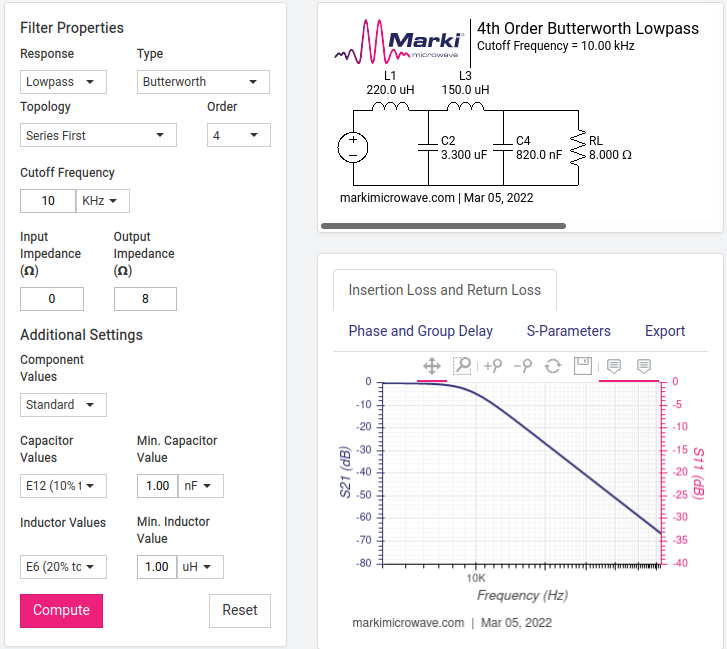
\includegraphics[width=\textwidth]{zvuk-D-butterworth}
    \caption{%
        Návrh filtru pro spínaný zesilovač ve webovém nástroji
        \url{https://rf-tools.com/lc-filter/}
    }
    \label{fig:zvuk D butterworth}
\end{figure}

\begin{figure}[hptb]
    \centering
    \begin{circuitikz}
        \draw
            (0,3) to [L, l=$L_1$, a=$\SI{220}{\micro\henry}$, o-] (3,3)
            to [C, l_=$C_1$, a^=$\SI{3,3}{\micro\farad}$] (3,0)
            to [short, -o] (0,0)
            (3,3) to [L, l=$L_2$, a=$\SI{100}{\micro\henry}$, *-] (6,3)
            to [C, l_=$C_2$, a^=$\SI{1}{\micro\farad}$] (6,0)
            to [short, -*] (3,0)
            (6,3) to [C, l=$C_3$, a=$\SI{220}{\micro\farad}$, *-o] (9,3)
            to [short] (10,3)
            to [loudspeaker, a^=$\SI{8}{\ohm}$] (10,0)
            to [short, -o] (9,0)
            to [short, -*] (6,0)
            (4.5,0) to [short, *-] ++(0,-0.1) node [ground] {}
            ;
    \end{circuitikz}
    \caption{%
        Schéma zapojení filtru pro spínaný zesilovač
    }
    \label{fig:zvuk D filtr sch}
\end{figure}

Umístění vazebního kondenzátoru $C_3$ odstraňujícího stejnosměrnou složku
signálu až na výstup filtru umožňuje použít jako $C_1$ a $C_2$ elektrolytické
kondenzátory, které mají při stejné kapacitě několikanásobně menší rozměry než
například kondenzátory fóliové. Napětí na nich je totiž při normálním provozu
vždy kladné. Vzhledem k malým potřebným kapacitám a provozním napětím ale
postačí i vícevrstvé keramické kondenzátory (MLCC).

Filtr tvořený dvěma cívkami a dvěma kondenzátory má dvě rezonanční frekvence,
při kterých může dojít k nežádoucímu nárůstu napětí na jeho součástkách. Při
připojené zátěži (reproduktor s impedancí \SI{8}{\ohm}) jsou kmity tlumené,
s odpojenou zátěží ale může dojít k výraznému nárůstu napětí například na
kondenzátorech filtru (viz obrázek~\vref{fig:zvuk D filtr sim graf}).
%V praxi se ale neprojevily žádné problémy způsobené touto nedokonalostí.
\todo{prakticky otestovat novy filtr}



\begin{figure}[htb]
    \centering
    \includegraphics[width=0.80\textwidth]{sim/cropped_zvuk-D-filtr.pdf}
    \caption{Simulace filtru pro spínaný zesilovač v programu LTspice}
    \label{fig:zvuk D filtr sim sch}
\end{figure}

\begin{figure}[htb]
    \centering
    \input{sim/graf-zvuk-D-filtr.tex}
    \caption{%
        Útlumová frekvenční charakteristika filtru dle simulace
        z~obrázku~\vref{fig:zvuk D filtr sim sch}
    }
    \label{fig:zvuk D filtr sim graf}
\end{figure}

\todo[inline]{dopsat spinany zesilovac}

\FloatBarrier
\paragraph{Bipolární tranzistor jako Zenerova dioda}
V souvislosti s problematikou vysokonapěťových špiček způsobených rezonancí ve
filtru spínaného zesilovače ve stavu odpojené zátěže (reproduktoru) byly
zkoumány metody jejich omezení. K tomuto účelu by byla vhodná Zenerova dioda,
to by ale znamenalo přidání dalšího typu součástky, který je nutné pro osazení
desky plošných spojů opatřit. Za účelem zachování co nejmenšího počtu různých
typů součástek byly prováděny experimenty s použitím běžného bipolárního
tranzistoru NPN, konkrétně jeho přechodu báze--emitor, jako Zenerovy diody.
U křemíkových tranzistorů totiž v závěrném směru dochází k průrazu tohoto
přechodu již od cca \SI{5}{\volt}. Pro účely omezení napěťových špiček
nepotřebujeme, aby bylo toto napětí přesné.

Pro ověření tohoto konceptu byl vytvořen jednoduchý testovací obvod sestávající
z generátoru funkcí FY6900, který umožňuje dosažení napětí až \SI{25}{\volt},
a~digitálního osciloskopu. Využíváme faktu, že výstupní impedance použitého
generátoru je \SI{50}{\ohm}.

\begin{figure}[htb]
    \centering
    \begin{circuitikz}
        \draw
            (4,3) node [npn] (npn) {BC546}
            (0,3) to [sinusoidal voltage source] (0,0)
            (0,3) to [R=$\SI{50}{\ohm}$] (2,3)
            to [short] (npn.B)
            (npn.E) to [short] (npn.E |- 0,0)
            to [short] (0,0)
            %
            (3,3) to [oscope, *-*] (3,0)
            ;
        \draw[thick, dash dot] (-1,4) rectangle (2.25,-0.5)
            (1,-0.5) node[below] {FY6900}
            ;
    \end{circuitikz}
    \caption{%
        Schéma zapojení obvodu pro testování možnosti využití NPN tranzistoru
        jako Zenerovy diody
    }
    \label{fig:tranzistor zenerka sch testing}
\end{figure}


\begin{figure}[htb]
    \centering
    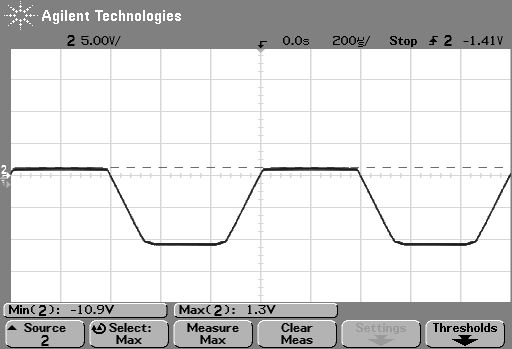
\includegraphics[width=0.8\textwidth]{scope-tranzistor-zenerka}
    \caption{%
        Sinusoida ze zdroje s výstupní impedancí \SI{50}{\ohm} oboustranně
        amplitudově omezená přechodem báze--emitor bipolárního tranzistoru
        BC546
    }
    \label{fig:tranzistor zenerka scope}
\end{figure}

Obvod pracuje dle očekávání, v závěrném směru dochází k nedestruktivnímu
průrazu při napětí \SI{-11}{\volt}. V měřeném rozsahu frekvencí do
\SI{50}{\kilo\hertz} nedochází k žádnému problematickému jevu. Pro výše popsaný
účel by tranzistor postačoval. Zajímavostí je, že simulační program LTspice
(a~programy SPICE obecně) používá model bipolárního tranzistoru, který průraz
přechodu báze--emitor neuvažuje.



\FloatBarrier  % TODO global ??
\subsection{Implementace zvukového výstupu ve firmware}
Generování obdélníkového signálu s určenou periodou je na MCU nejjednodušeji
proveditelné s využitím hardwarové periferie čítače/časovače. V této práci
využitý MCU má těchto periferií několik, pro účely implementace zvukového
výstupu je ale nejvhodnější 16bitový Timer1.

Protože je cílem generovat sinusový signál, musí se perioda PWM signálu v čase
měnit. Toho můžeme dosáhnout periodickým přepisováním hodnoty registru
určujícího střídu. Pro sinusové signály vyšších frekvencí musíme tyto změny
střídy provádět s periodou kratší než jeden průchod hlavní smyčkou. Proto
musíme využít přerušení a hodnotu střídy přepisovat v obslužné rutině ISR.
Toto přerušení potřebujeme spouštět periodicky, tedy při přetečení jednoho
z časovačů. Vhodnou volbou délky běhu časovače Timer1 můžeme dosáhnout toho, že
tento časovač bude vhodný jak pro generování PWM signálu, tak i pro spouštění
ISR.

\subsubsection{Testovací verze}
Pro prvotní ověření konceptu byl vytvořen jednoduchý firmware implementující
pouze zvukový výstup. V repositáři \gitrepo{AlarmClock} je umístěn v adresáři
\repopath{development/audio}.  % POZOR tuhle cestu mozna zmenim (platformio)

Aby se testovací implementace přiblížila kódu, který by bylo možné zahrnout do
hlavního firmware, je pojata formou knihovny v jazyce \texttt{C} a jednoduchého
Arduino projektu \filename{audio.ino}, který knihovnu využívá.

Hlavičkový soubor \filename{PWMSine.h} definuje API knihovny a je naprosto
triviální:
\begin{lstlisting}[language=C++,style=numbers]
#ifndef PWMSINE_H
#define PWMSINE_H

// PWM period. 20 us (50 kHz) seems to be optimal for further signal
// processing.
#define timer1_us 20

void PWMSine_setup();
void PWMSine_tone(uint8_t pin, uint16_t freq, uint8_t amplitude=255);
void PWMSine_noTone(uint8_t pin);

#endif  // PWMSINE_H
\end{lstlisting}

Knihovna implementuje pouze tři funkce~--
\lstinline[language=C]!void PWMSine_setup()! provádí inicializaci časovače.
\lstinline[language=C]!void PWMSine_tone(uint8_t pin, uint16_t freq, uint8_t amplitude=255)!
zahajuje generování sinusového signálu na výstupním pinu \texttt{pin} (na desce
Arduino UNO jsou použitou knihovnou \texttt{TimerOne} podporované piny 9
a~10~\cite{TimerOnedocs}). Generovaný signál má frekvenci \texttt{freq} a jeho
amplituda je určena 8bitovým číslem \texttt{amplitude}.
\lstinline[language=C]!void PWMSine_noTone(uint8_t pin)! ukončuje generování
tónu na výstupním pinu \texttt{pin}.

Vlastní definice funkcí se nachází v souboru \filename{PWMSine.cpp}:
\begin{lstlisting}[language=C++,style=numbers]
// https://github.com/PaulStoffregen/TimerOne
// version 1.1.0 (git tag 1.1)
#include <TimerOne.h>

#include "PWMSine.h"
#include "sinlut.h"

uint8_t tone_pin;
uint8_t tone_amplitude;
// number of sine wave points per interrupt * 64
// (*64 increases resolution)
uint16_t tone_k;


void timer1_ISR()
{
    static uint16_t i = 0;
    i += tone_k;
    int16_t value = int8_t(pgm_read_byte_near(sin_LUT + (uint8_t)(i/64))) * tone_amplitude / 64;
    Timer1.setPwmDuty(tone_pin, value + 512);
}


void PWMSine_setup()
{
    Timer1.initialize(timer1_us);
    Timer1.stop();
    Timer1.attachInterrupt(timer1_ISR);
}


void PWMSine_tone(uint8_t pin, uint16_t freq, uint8_t amplitude)
{
    tone_k = 64UL * timer1_us * 256UL / (1000000UL/freq);
    tone_pin = pin;
    tone_amplitude = amplitude;
    // Timer1.pwm needs to be called at least once before setPwmDuty can be
    // used.
    Timer1.pwm(tone_pin, 512);
    Timer1.start();
}


void PWMSine_noTone(uint8_t pin)
{
    (void)pin;
    Timer1.stop();
}
\end{lstlisting}

Pro generování PWM signálu je využit 16bitový časovač použitého MCU -- Timer1.
Knihovna \texttt{TimerOne} zprostředkovává jednodušší ovládání této periferie.
Odkaz na její zdrojový kód a specifikace použité verze jsou uvedeny jako
komentář na začátku souboru \filename{PWMSine.cpp}. Jde o svobodnou knihovnu
dostupnou pod podmínkami licence
\foreignlanguage{english}{Creative Commons Attribution 3.0 United States
License}~\cite{TimerOnerepo}.

Funkce \verb|PWMSine_setup| provádí inicializaci časovače a nastavuje periodu
čítání na hodnotu \verb|timer1_us|, tedy \SI{20}{\micro\second}. Poté
zastavuje časovač a nastavuje, aby byla při jeho přetečení zavolána funkce
\verb|timer1_ISR|.

Funkce \verb|PWMSine_tone| nastavuje globální proměnnou \verb|tone_k| na
hodnotu vypočítanou z požadované frekvence sinusového signálu.
Poté nastavuje proměnnou \verb|tone_pin| na hodnotu určenou parametrem
\texttt{pin}. To je nutné, protože tuto hodnotu využíváme ve funkci
\verb|timer1_ISR|. To samé platí pro proměnnou \verb|tone_amplitude|.
Následně zahajuje generování PWM signálu se střídou \SI{50}{\percent} na
výstupním pinu \verb|tone_pin| a zahajuje běh časovače Timer1.

Funkce \verb|PWMSine_noTone| sice přijímá jako parametr výstupní pin,
v současné implementaci ale tuto hodnotu nevyužívá. Aby se zamezilo varování
kompilátoru \shellcmd{gcc} \uv{\foreignlanguage{english}{unused parameter}},
je využita konstrukce jazyka \texttt{C}, která varování při kompilaci potlačí,
ale neprojeví se na generovaném strojovém kódu:
\begin{lstlisting}[language=C]
(void)pin;
\end{lstlisting}
Jediným projevem funkce je tak zastavení časovače Timer1.

Funkce \verb|timer1_ISR| je volána v důsledku hardwarového přerušení,
tedy nezávisle na běhu programu. Protože k tomuto přerušení dochází každých
\SI{20}{\micro\second}, musí mít tato funkce na úrovni strojového kódu co
nejméně instrukcí, aby se minimalizovalo zpomalení běžných operací prováděných
v hlavní smyčce firmware. Funkce při každém zavolání nastavuje 16bitové číslo
$i$ na $i + \mathrm{tone_k}$. Poté určuje výpočtem požadovanou střídu PWM
signálu $\mathrm{value}+512$, kterou nastavuje na používaném časovači. Střída
je 10bitové číslo, nabývá tedy hodnot od \num{0} do \num{1023}. Pro nastavení
střídy PWM signálu je využita metoda \texttt{Timer1.setPwmDuty}, která akci
provede rychleji než \texttt{Timer1.pwm}. \texttt{Timer1.pwm} se ale musí
zavolat alespoň jednou před použitím \texttt{Timer1.setPwmDuty}, protože
provádí inicializaci.~\cite[ověřeno praktickým pokusem]{TimerOnedocs}

Výpočet hodnoty $\mathrm{value}$ určující střídu $\mathrm{value}+512$ pouze
implementuje následující funkci:
\begin{equation}
    d(t) = \num{0,5} + \frac{A}{2} \cdot \sin{(2\pi f t)}
    \label{eq:duty float}
\end{equation}
kde $0 \le d \le 1$ je střída, $f$ je požadovaná frekvence, $0 \le A \le 1$ je
požadovaná amplituda a $t$ je doba uplynulá od začátku generování signálu.

Výpočty s desetinnými čísly s pohyblivou řádovou čárkou by ale byly příliš
pomalé pro použití v ISR, proto jsou využity celočíselné proměnné. Část
výpočtů je též odsunuta do funkce \verb|PWMSine_tone| -- viz proměnná
\verb|tone_k|.

Střída PWM signálu je určena hodnotou funkce $\sin$. Matematické určování
těchto hodnot za běhu programu přímo na MCU by ale bylo příliš časově náročné.
Proto je využita vyhledávací tabulka (LUT) \filename{sinlut.h}, která obsahuje
hodnoty funkce $\sin$ jako 8bitové číslo se znaménkem pro 256 hodnot argumentu
od $0$ do $2\pi$. Tato LUT je generována jednoduchým programem napsaným
v jazyce \texttt{Python}~-- \filename{sinlut.py}~-- spouštěným na standardním
počítači před kompilací firmware:
\begin{lstlisting}[language=Python,style=numbers]
#!/usr/bin/env python3
"""Generate sinlut.h"""

import math

header = """/*!
    @file
    @brief Lookup table for sin.

    This file is automatically generated by `sinlut.py`.
*/

#ifndef SINLUT_H
#define SINLUT_H

const int8_t PROGMEM sin_LUT[] = {
"""

footer = """};

#endif  // SINLUT_H
"""


if __name__ == '__main__':
    with open('sinlut.h', 'w') as f:
        f.write(header)
        for i in range(0, 256):
            value = int(math.sin(2*math.pi / 256 * i) * 127)
            f.write(f'    {value},  // {i}\n')
        f.write(footer)
\end{lstlisting}

Výstupem je soubor \filename{sinlut.h}:
\begin{lstlisting}[language=C++,style=numbers]
/*!
    @file
    @brief Lookup table for sin.

    This file is automatically generated by `sinlut.py`.
*/

#ifndef SINLUT_H
#define SINLUT_H

const int8_t PROGMEM sin_LUT[] = {
    0,  // 0
    3,  // 1
    6,  // 2
    // ...
    -6,  // 254
    -3,  // 255
};

#endif  // SINLUT_H
\end{lstlisting}

Vzorec pro výpočet hodnot funkce $\sin$ pro účely vytvoření LUT je následující:
\begin{equation}
    a(i) = \operatorname{int}\left( \num{127}\cdot\sin{\left(2\pi \cdot \frac{i}{256}\right)} \right)
\end{equation}
kde $\num{-127} \le a \le \num{127}$ je výstupní hodnota pro LUT
a~$\num{0} \le i \le \num{255}$ je pořadí hodnoty $a$ v LUT. Hodnota $a$ je
přetypována na celé číslo ($\operatorname{int}$), desetinná část je tedy
ignorována.

Arduino projekt \filename{audio.ino} je velmi primitivní a pouze využívá funkce
výše popsané knihovny ke generování testovacích signálů:
\begin{lstlisting}[language=C++,style=numbers]
#include "PWMSine.h"

#define pin_speaker 9  // needs to be supported by TimerOne

void setup()
{
    PWMSine_setup();
}


void loop()
{
    PWMSine_tone(pin_speaker, 440, 128);
    delay(1000);
    PWMSine_tone(pin_speaker, 440, 255);
    delay(1000);
    PWMSine_noTone(pin_speaker);
    delay(2000);
}
\end{lstlisting}
Generované signály jsou sinusoida o frekvenci \SI{440}{\hertz} s poloviční
amplitudou po dobu $\SI{1000}{\milli\second} = \SI{1}{\second}$, sinusoida
o frekvenci \SI{440}{\hertz} s plnou amplitudou po dobu \SI{1}{\second} a ticho
po dobu \SI{2}{\second}. Poté se smyčka opakuje.


\subsubsection{Plná verze}
Implementace ve firmware budíku je mírně odlišná. Knihovna \filename{PWMSine.h}
definuje \texttt{C++} třídu \texttt{PWMSine} a její vnitřní kód je v porovnání
s testovací verzí složitější. API knihovny je dokumentováno standardně
technologií \shellcmd{doxygen}.

Oproti testovací verzi přibyla metoda
\lstinline[language=C++]!void PWMSine::silence(uint8_t pin)!, která slouží ke
generování ticha. Kdyby byla místo této metody využita metoda \texttt{noTone},
došlo by k úplnému vypnutí PWM výstupu a výstupní pin by přešel do úrovně
logické~0. To by v reproduktoru způsobilo slyšitelné cvaknutí, protože do té
doby zpracovávaný sinusový signál měl stejnosměrnou složku \SI{2,5}{\volt} a na
tuto hodnotu byl nabit i vazební kondenzátor. Náhlá změna stejnosměrné složky
signálu na \SI{0}{\volt} při vypnutí zvukového výstupu ve firmware se tak na
vstupu lineárního zesilovače (za vazebním kondenzátorem) projeví jako impuls se
špičkou \SI{-2,5}{\volt} -- viz obrázek \vref{fig:zvuk silence sim}. (Poznámka:
ve skutečném obvodu s lineárním zesilovačem je před vazebním kondenzátorem
zařazen atenuátor, takže špička dosahuje pouze zlomku amplitudy
\SI{-2,5}{\volt}. Pro účely vysvětlení tohoto problému ale postačí atenuátor
ignorovat.)

\begin{figure}[htb]
    \centering
    \begin{circuitikz}
        \draw
            (0,3) to [sqV, l=$\SI{1,25}{\volt}$] (0,1.5)
            to [V=$\SI{1,25}{\volt}$] (0,0)
            (0,3) to [short] (2,3)
            to [C=$C_\mathrm{v}$,a=$\SI{100}{\nano\farad}$] (5,3)
            to [R,a=$\SI{1}{\kilo\ohm}$,v^=$u_2$] (5,0)
            to [short] (0,0)
            (2,3) to [open, v^=$u_1$] (2,0)
            ;
    \end{circuitikz}
    \input{sim/graf-zvuk-silence.tex}
    \caption{%
        Schéma zapojení a výsledek počítačové simulace obvodu demonstrujícího
        problémy se cvakáním zvukového výstupu při použití metody
        \texttt{noTone}
    }
    \label{fig:zvuk silence sim}
\end{figure}

Úplné vypnutí zvukového výstupu metodou \texttt{noTone} je sice žádoucí při
ukončení buzení, například během přerušovaného pískání ale působí rušivě.
Objekt \texttt{BuzzerManager} proto v takových případech využívá právě metodu
\texttt{silence}, která na výstupním pinu generuje PWM signál o konstantní
střídě \SI{50}{\percent}.


\paragraph{Příkazy v \texttt{AlarmClockCLI}}
V příkazovém řádku (CLI) budíku byly implementovány příkazy umožňující
jednoduché testování zvukového výstupu. V nápovědě jsou zdokumentovány
následovně:
\begin{lstlisting}[style=terminal]
Help:
  ...
  Sound (testing only):
    tone{f/10};{a}
    silence
    notone
  ...
\end{lstlisting}

Implementace těchto příkazů je velmi jednoduchá. Pokud je firmware zkompilován
s definicí \verb|acite_buzzer|, pouze vrátí chybu \verb|Unsupported|. Pokud je
firmware zkompilován bez této definice, volají příslušné funkce
z~\verb|PWMSine|. Frekvence předávaná příkazu \verb|tone| musí být vydělena 10,
protože v opačném případě by délka tohoto příkazu mohla přesáhnout délku paměti
pro CLI příkazy. Upravit délku paměti by bylo triviální, ale protože jde
o příkaz určený pouze pro testování, bylo zvoleno zkrácení příkazu.

CLI příkazy pro ovládání zvukového výstupu jsou určené pouze pro testování,
protože je s jejich pomocí možné uvést zvukový výstup do stavu, který nelze
s použitím standardních ovládacích prvků opustit.



\paragraph{Melodie}
V průběhu vývoje vyvstal požadavek na možnost změnit frekvenci periodu
a hlasitost přerušovaného pískání při buzení. Vzhledem k jednoduchosti
implementace bylo zvoleno flexibilnější řešení, které umožňuje vytváření
jednoduchých melodií a přiřazování těchto melodií jednotlivým budicím časům.

Melodii můžeme pro účely tohoto projektu definovat jako seznam tónů, které se
postupně přehrávají. Každý tón je charakterizován svou frekvencí, amplitudou
a délkou trvání. Není potřeba definovat speciální případ pro pomlky (období
ticha), protože pro tyto účely můžeme využít tón o libovolné frekvenci
s amplitudou rovnou nule.

Melodie musí být v mikrokontroléru ukládány tak, aby nedošlo k jejich ztrátě
při ztrátě napájení. To vylučuje jejich ukládání v paměti SRAM. Bylo by možné
využít programovou paměť Flash, to by ale vylučovalo jednoduché přepisování
uložených dat za normálního běhu programu (firmware). Proto byla zvolena
interní paměť EEPROM.

Pro ukládání melodií v paměti EEPROM byl vytvořen následující binární formát:
Každá melodie má 3bytovou hlavičku. Hlavička první melodie začíná v EEPROM na
adrese \texttt{0x0010} (definováno konstantou
\verb|EEPROM_melodies_header_start|), následují hlavičky ostatních melodií.
Celkový počet melodií je 16. Hlavička melodie je reprezentována binárními daty
dle následujících pravidel:
\begin{itemize}[nosep]
    \item První byte obsahuje informace o melodii. Jeho nejméně významný bit
        (LSB, bit 0) vždy nabývá hodnoty logické 1. Následující bit nabývá
        hodnoty 1, pokud je melodie aktivovaná. Zbývající bity 2 až 7 jsou
        nevyužité a na jejich hodnotě nezáleží.
    \item Druhý a třetí byte udávají adresu paměti EEPROM, na které začínají
        data dané melodie. Adresa je ukládána jako 16bitové slovo v pořadí bytů
        little-endian.
\end{itemize}

Data melodie začínají 3 byty o hodnotách \texttt{0xFD}; \texttt{0x55};
\texttt{0xAA}. Následuje libovolný počet 3bytových tónů. Data jsou zakončena 3
byty o hodnotě \texttt{0x00}. Validní tón má nenulovou délku trvání, proto se
tato sekvence nemůže vyskytnout uvnitř dat, které ji předchází. Následuje byte
o hodnotě \texttt{0xFF} a 1bytové slovo, jehož LSB je nastaven na 1, pokud se
má po prvním přehrání melodie opakovat. Ostatní bity tohoto slova jsou
nevyužité. Další 3 jednobytová čísla bez znaménka jsou přičtena k amplitudě
všech tónů při 2., 3. a 4. opakování melodie. Třetí číslo je využito i pro 5.
a další opakování. Pokud je amplituda tónu v melodii 0, není toto číslo
přičteno. Pokud je amplituda tónu po přičtení čísla z patičky větší než
\num{255}, je použita hodnota \num{255}, aby se při aritmetické operaci
zabránilo nechtěnému přetečení.

Pokud není patička melodie validní nebo pokud je v hlavičce zapsáno, že melodie
není aktivována, přepne se budík do režimu standardního přerušovaného pípání.
To zajišťuje, že nemůže dojít k tichému přehrávání nevalidních dat.

Každý tón je reprezentován 3 jednobytová čísla bez znaménka:
\begin{itemize}[nosep]
    \item frekvence: $\frac{f - \SI{32}{\hertz}}{\SI{32}{\hertz}}$,
    \item amplituda: \num{0} je ticho, \num{255} je plná hlasitost,
    \item délka trvání: $\frac{t}{\SI{25}{\milli\second}}; t > 0$.
\end{itemize}

Vzorce pro výpočet hodnot uložených v paměti z požadovaných parametrů tónu
vychází z omezení ukládaných čísel na rozsah \numrange{0}{255}.
Vzorec pro přepočet frekvence umožňuje vytváření tónů o frekvencích od
\SI{32}{\hertz} do \SI{8,192}{\kilo\hertz} s rozlišením \SI{32}{\hertz}.
Volba minimální frekvence vychází z původní implementace pomocí funkce \verb|tone|
Volba vzorce pro délku trvání vychází z původního zamýšleného využití
melodií~-- definice vlastního přerušovaného pískání. Je tedy důležité, aby bylo
možné definovat dlouho trvající tóny. Rozsah je \SI{25}{\milli\second} až
\SI{6,375}{\second} s rozlišením \SI{25}{\milli\second}. Podmínka, že délka
trvání tónu nesmí být nulová, umožňuje využít 3 po sobě jdoucí byty s hodnotou
\texttt{0x00} pro zakončení dat v paměti.

Pro testování melodií byly též vytvořeny nové příkazy v CLI:
\begin{lstlisting}[style=terminal]
Help:
  ...
  Melodies:
    melody{i} - play melody 0-15
  EEPROM:
    eer{aaaa} - read data from address
    eew{aaaa};{ddd} - write data to address
  ...
\end{lstlisting}

Příkaz \verb|melody| slouží k zahájení přehrávání vybrané melodie
(\numrange{0}{15}), při použití bez parametru přehrávání ukončuje.
Pro manipulaci s daty v paměti EEPROM byl implementován příkaz
\verb|eer| sloužící ke čtení jednoho bytu z určené adresy a \verb|eew|
provádějící zápis jednoho bytu dat na určitou adresu. Příklad použití nových
příkazů pro práci s daty v EEPROM:
\begin{lstlisting}[style=terminal]
> eer 1023
---
EEPROM:
  1023: 255
...

err 0x0: OK

> eew 1023;10

err 0x0: OK

> eer 1023
---
EEPROM:
  1023: 10
...

err 0x0: OK

> eer 1024

Processing

err 0x1: Invalid args

>
\end{lstlisting}

Pro zjednodušení použití těchto příkazů byl vytvořen program
\shellcmd{EEPROM-tool.py} (umístěný ve složce \repopath{examples/} v repositáři
\gitrepo{PyAlarmClock}). Ten umožňuje přečtení souvislého bloku dat z EEPROM
a zápis do binárního souboru, nebo naopak zápis dat z binárního souboru do
EEPROM. Například přečtení hlaviček všech melodií do souboru
\texttt{hlavicky.bin} provádíme následovně:
\begin{lstlisting}[style=terminal]
$ EEPROM-tool.py /dev/ttyUSB0 read 0x0010 48 hlavicky.bin
INFO:PyAlarmClock:Initializing serial port
100%|#####################| 48/48 [00:03<00:00, 13.09it/s]
$ ls -l hlavicky.bin
-rw-rw-r-- 1 ondra ondra 48 2022-01-07 15:43 hlavicky.bin
$ xxd hlavicky.bin
00000000: 0300 0103 1001 0000 0000 0000 0000 fe00  ................
00000010: 0000 0000 0000 0000 fe00 0000 0000 0000  ................
00000020: 0000 fe00 0000 0000 0000 0000 fe00 0000  ................
$
\end{lstlisting}

Manuální úpravy binárního souboru přečteného z EEPROM jsou zdlouhavé, protože
je nutné neustále nahlížet do dokumentace a dekódovat význam jednotlivých bytů.
Proto je výhodné využít editor binárních dat GNU
\shellcmd{poke}\footnote{\url{http://www.jemarch.net/poke}} implementující
doménově specifický programovací jazyk
Poke\footnote{\url{http://jemarch.net/pokology-01102019.html}}.
Struktura dat je popsána souborem zvaným \texttt{pickle}. Po načtení tohoto
\texttt{pickle} do interaktivního příkazového řádku \shellcmd{poke} provádíme
mapování dané struktury na konkrétní data v binárním souboru a dále s nimi
pracujeme jako s objekty. Celý pickle je uložen v souboru
\repopath{tools/AlarmClockEEPROM.pk} v repositáři \gitrepo{AlarmClock}, pro
demonstraci konceptu ale použijeme pouze jeho část:
\begin{lstlisting}[language=Poke]
/*
 * Melodies
 */

set_endian(ENDIAN_LITTLE);

type EEPROM_melody_header = struct {
    uint<6>;
    uint<1> enabled;
    uint<1> valid = 1;
    uint<16> data_address;
    method _print = void:
    {
        print "#<\n";
        printf "  enabled: %s\n", enabled ? "yes" : "no";
        printf "  address: 0x%u16x\n", data_address;
        print ">";
    }
};
\end{lstlisting}

Spustíme \shellcmd{poke} a jako parametr mu předáme název binárního souboru~--
\texttt{hlavicky.bin}. Přepínač \texttt{-l} slouží k načtení pickle při
spuštění. Vytvoříme novou proměnnou \verb|melody_headers| jako pole struktur
\verb|EEPROM_melody_header| začínající na začátku souboru (\verb|@ 0#B|). Počet
prvků v poli je určen dynamicky -- prvky se přidávají, dokud se nenarazí na
konec souboru nebo dokud nejde k porušení omezení (\texttt{constraint}).
Protože v našem souboru \texttt{hlavicky.bin} nejsou všechny hlavičky melodií
validní, má pole pouze 2 prvky.
\begin{lstlisting}[style=terminal]
$ poke -l ~/source/repos/AlarmClock/tools/AlarmClockEEPROM.pk hlavicky.bin
     _____
 ---'   __\_______
            ______)  GNU poke 1.0
            __)
           __)
 ---._______)

Copyright (C) 2019-2021 The poke authors.
License GPLv3+: GNU GPL version 3 or later <http://gnu.org/licenses/gpl.html>.
This is free software: you are free to change and redistribute it.
There is NO WARRANTY, to the extent permitted by law.

Powered by Jitter 0.9.258.
Perpetrated by Jose E. Marchesi.

For help, type ".help".
Type ".exit" to leave the program.
+ (poke) var melody_headers = EEPROM_melody_header[] @ 0#B
+ (poke) melody_headers
[EEPROM_melody_header {(uint<6>) 0,enabled=(uint<1>) 1,valid=(uint<1>) 1,data_address=256UH},EEPROM_melody_header {(uint<6>) 0,enabled=(uint<1>) 1,valid=(uint<1>) 1,data_address=272UH}]
+ (poke) .set pretty-print yes
+ (poke) melody_headers
[#<
  enabled: yes
  address: 0x0100
>,#<
  enabled: yes
  address: 0x0110
>]
+ (poke)
\end{lstlisting}
Příkaz \verb|.set pretty-print yes| zapnul uživatelsky přívětivé vypisování,
které volá metody \verb|_print| daných struktur.

S pomocí \shellcmd{poke} bychom mohli například snadno upravit adresu dat
v první hlavičce (\lstinline[language=Poke]|melody_headers[0].address = 0x0123|)
a s pomocí \shellcmd{EEPROM-tool.py} binární soubor zapsat zpět do paměti
EEPROM.


% Zajimave zdroje (nepouzito, necituji):
% https://uu.diva-portal.org/smash/get/diva2:1219146/FULLTEXT01.pdf

\section{Stmívaný zdroj světla}
K~budíku lze připojit zdroj světla (ve firmware je tato funkce nazývána
\texttt{ambient}), který je pozvolna rozsvěcen před zahájením akustického
buzení. Cílem je napodobovat postupné rozednění.

Na výstupu \MCUpin{PD6} mikrokontroléru je PWM signál o~frekvenci
\SI{980}{\hertz}\footnote{\url{https://www.arduino.cc/reference/en/language/functions/analog-io/analogwrite/}}.
Na většině ostatních výstupních pinů by byla frekvence \SI{490}{\hertz}, piny 5
a~6 jsou v~tomto výjimečné. % Pouze uno, na MEGA piny 4 a 13
Přímé řízení samostatné výkonové LED či LED pásku tímto signálem by způsobovalo
blikání světla na této frekvenci, proto je vhodnější plynule regulovat proud
protékající LED napájenou zdrojem konstantního proudu.
% https://electronics.stackexchange.com/questions/277238/disadvantages-of-dimming-leds-via-current-regulation-as-opposed-to-via-pulse-fre


\subsection{Testovací verze}
Pro prvotní ověření užitečnosti celého konceptu byl vytvořen jednoduchý
tranzistorový obvod, který slouží k~napájení jedné LED o~jmenovitém výkonu
\SI{1}{\watt} ze zdroje o~napětí \SI{12}{\volt}. Obvod je určen pouze pro
testování a~při jeho návrhu proto nebylo věnováno příliš pozornosti tomu, aby
byla závislost proudu protékajícího LED na střídě PWM signálu lineární (viz
graf na obrázku~\vref{fig:ambient linear testing sim napeti}).
Z~tohoto důvodu není obvod vhodný pro použití ve finálním výrobku. Dalšími
nevýhodami jsou nízká účinnost, potřeba chladit výkonový tranzistor a~z~toho
vyplývající velké fyzické rozměry součástek. Obvod ale lze velmi snadno
sestavit na nepájivém kontaktním poli.

Výkonovou LED v~pouzdře pro povrchovou montáž je nutné chladit, pro testování
prototypů lze využít výrobcem dodaný chladič. Jde o~malou desku plošných spojů
s~hliníkovým podkladem. Pro odvod tepla má LED na spodní straně plochu pro
připájení k~chladiči. To znemožňuje pájení standardní mikropáječkou, spodní
strana součástky totiž není při pájení přístupná. Vhodnější metodou je
aplikování pájecí pasty (tavidla s~obsahem pájky) a~zahřátí celé desky na
teplotu pájení. Pájení horkým vzduchem by zbytečně tepelně namáhalo horní
stranu LED (např. čočku), proto je vhodnější aplikovat teplo ze spodní strany
(viz obrázek~\vref{fig:ambient LED pajeni}).

\begin{figure}[htbp]
    \centering
    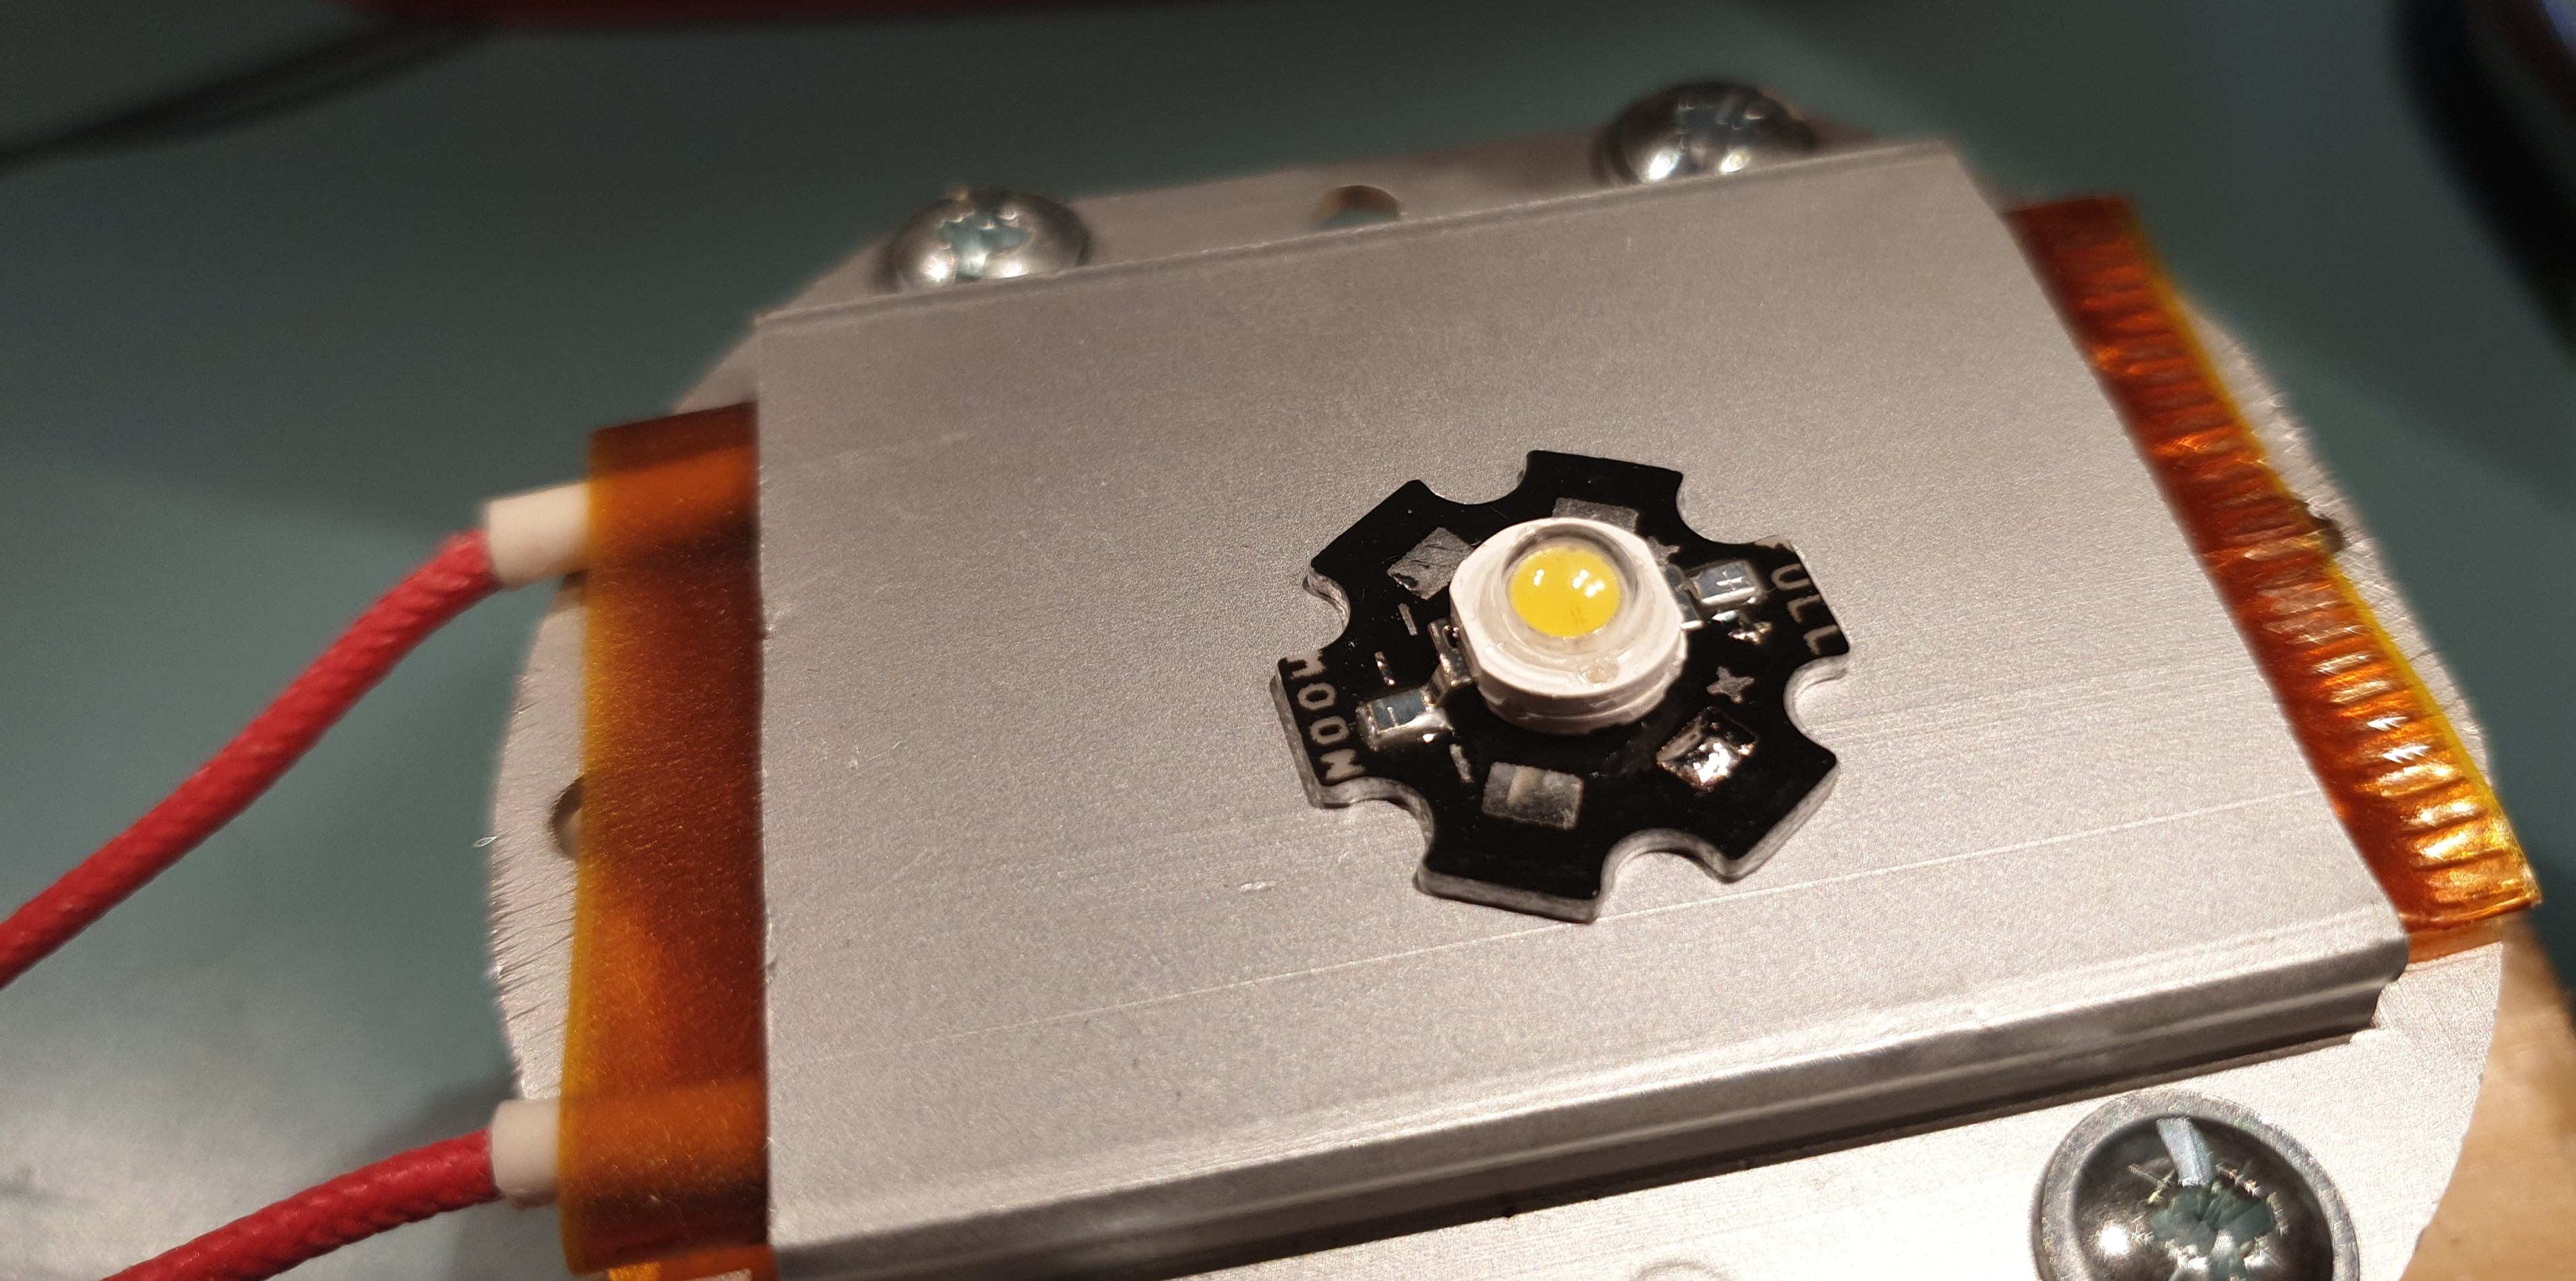
\includegraphics[width=0.6\textwidth]{ambient-LED-pajeni}
    \caption{Pájení výkonové SMD LED na chladič}
    \label{fig:ambient LED pajeni}
\end{figure}



\begin{figure}[htbp]
    \centering
    \includegraphics[width=0.9\textwidth]{cropped_ambient-linear-testing}
    \caption{Schéma zapojení testovacího lineárního stmívače pro výkonovou LED}
    \label{fig:ambient linear testing sch}
\end{figure}

\begin{figure}[htbp]
    \centering
    \subcaptionbox{%
        Schéma zapojení a~nastavení simulace%
        \label{fig:ambient linear testing sim sch}
    }{%
        \includegraphics[width=0.9\textwidth]{sim/cropped_ambient-linear-testing}%
    }
    \subcaptionbox{%
        Závislost proudu protékajícího LED na napětí zdroje V1 reprezentujícího
        kondenzátor $C_1$ z~obrázku~\vref{fig:ambient linear testing sch}%
        \label{fig:ambient linear testing sim napeti}
    }{%
        \input{sim/graf-ambient-linear-testing.tex}%
    }
    \caption{Simulace testovacího lineárního stmívače v~programu LTspice}
    \label{fig:ambient linear testing sim}
\end{figure}

Vstupní PWM signál je převáděn na analogové napětí dolní propustí (integračním
článkem RC tvořeným R1 a~C1). Rezistory R2 a~R3 určují střídu PWM
signálu, při které se LED začne rozsvěcet a~při jaké střídě dosáhne plného
jasu. Tranzistor Q2 je použit kvůli nízkému proudovému zesilovacímu činiteli
tranzistoru Q3, se kterým tvoří darlingtonovo zapojení. Tranzistor Q3 reguluje
proud protékající LED (D1). Z~důvodu poměrně velkého ztrátového výkonu na této
součástce byl použit tranzistor KUY12 v~pouzdře TO-3. Rezistor R4 převádí
velikost proudu protékajícího větví s~LED na napětí. Velikost odporu tohoto
rezistoru určuje konstantní proud při plném jasu, protože tranzistor Q1 na
tomto rezistoru udržuje přibližně
konstantní úbytek napětí ($U_\mathrm{CE} \cong \SI{700}{\milli\volt}$).
Konstantní proud je tedy $I = \frac{U_\mathrm{CE}}{R_4} =
\frac{\SI{700}{\milli\volt}}{\SI{6,8}{\ohm}} \doteq \SI{103}{\milli\ampere}$.
Regulace probíhá přivíráním Q3.

\FloatBarrier
\subsection{Konečná verze}
Na finální verzi stmívače jsou přísnější požadavky:
\begin{itemize}[nosep]
    \item Obvod musí pracovat při napájecím napětí \SI{5}{\volt}.
    \item Při nulové střídě PWM signálu $d = \SI{0}{\percent}$ musí být LED
        zcela zhasnutá.
    \item Při střídě $d = \SI{100}{\percent}$ musí být proud protékající LED
        udržován na bezpečné konstantní hodnotě, nezávisle na velikosti
        napětí na LED a~napájecího napětí.
    \item Závislost proudu protékajícího LED (a~tedy i~její svítivosti) na
        střídě PWM signálu musí být přibližně lineární, rozsah
        $\SI{0}{\percent} \le d \le \SI{100}{\percent}$ musí být co nejlépe
        využit za současného zachování jednoduchosti obvodového řešení.
    \item Tepelné ztráty regulačního obvodu nesmí být příliš velké, aktivní
        i~pasivní součástky by se měly obejít bez rozměrných chladičů.
\end{itemize}

Vycházíme z~obvodu dle obrázku~\vref{fig:ambient linear testing sch} a~dále jej
zdokonalujeme. Aby nedošlo k~dosažení maximálního jasu příliš brzy, můžeme
zvýšit napětí na rezistoru R4, při kterém dochází k~omezování proudu. Toho lze
dosáhnout přidáním polovodičové diody D2 v~propustném směru mezi emitor Q1
a~zem. Střídu, při které se začne LED rozsvěcet, můžeme zmenšit přidáním
rezistoru mezi zdroj napětí \SI{5}{\volt} a~bázi Q2. Nechtěným oscilacím
zabráníme přidáním kondenzátoru mezi bázi Q2 a~zem. Hodnota jeho kapacity není
kritická, postačí běžná hodnota \SI{100}{\nano\farad}.

Praktickým zapojením bylo zjištěno, že výkonová LED svítí i~při velmi malých
proudech v~řádu stovek \si{\nano\ampere}. Její svit při požadovaném jasu
\SI{0}{\percent} lze eliminovat připojením rezistoru paralelně k~ní. Hodnota
odporu rezistoru není kritická, pro zhasnutí stačil i~odpor
\SI{100}{\kilo\ohm}. Na plošném spoji je osazen rezistor s~odporem
\SI{10}{\kilo\ohm}. Na funkci zbytku obvodu stmívače má tento odpor
zanedbatelný vliv a~ve schématu na
obrázku~\vref{fig:ambient linear prod sim sch} proto není zobrazen.

\begin{figure}
    \centering
    \subcaptionbox{%
        Schéma zapojení a~nastavení simulace%
        \label{fig:ambient linear prod sim sch}
    }{%
        \includegraphics[width=0.9\textwidth]{sim/cropped_ambient-linear-prod}%
    }
    \subcaptionbox{%
        Závislost proudu protékajícího LED na napětí zdroje V1%
        \label{fig:ambient linear prod sim napeti}
    }{%
        \input{sim/graf-ambient-linear-prod.tex}%
    }
    \caption{Simulace konečné verze lineárního stmívače v~programu LTspice}
    \label{fig:ambient linear prod sim}
\end{figure}

\subsubsection{Měření závislosti proudu protékajícího LED na střídě}
Pro prvotní experimenty dobře poslouží počítačová simulace v~programu
LTspice, dříve či později je ale potřeba navržené řešení vyzkoušet v~praxi.
Není absolutně nutné použít stejné typy tranzistorů jako na plošném spoji, tam
budou pravděpodobně použity součástky SMD, které ale nelze snadno připojit
k~nepájivému poli. Namísto SMD tranzistoru BC847 lze například použít BC547 či
BC546.

Proměřování charakteristik metodou bod po bodu opakované při každé změně
zapojení by bylo velmi zdlouhavé, proto byla vyvinuta jednodušší metoda jejich
měření.

Pro nahrazení PWM signálu vycházejícího z~\acs{MCU} je využit laboratorní
generátor funkcí FY6900. Jde o~dvoukanálový generátor využívající přímé
digitální syntézy (DDS) s~rozlišením 14 bitů a~vzorkovací frekvencí
\SI{250}{\mega\sample\per\second}. Pro účely tohoto měření využijeme funkci
rozmítání střídy. Generátor je nastaven tak, aby generoval na kanálu 1
obdélníkový signál (\texttt{Rectangle}) o~frekvenci \SI{1}{\kilo\hertz} (volba
frekvence není kritická) s~amplitudou \SI{5}{\volt} špička-špička a~offsetem
\SI{2,5}{\volt}. Stiskem tlačítka \texttt{SWEEP} je zvolena funkce rozmítání,
u~které jsou nastaveny následující parametry: lineární rozmítání střídy,
počáteční hodnota \SI{1}{\percent}, konečná hodnota \SI{99}{\percent}, čas
rozmítání \SI{20}{\second}, po dosažení konečné hodnoty skokový návrat na
počáteční hodnotu.
%\begin{lstlisting}[style=terminal]
%SWEEP:
%    OBJECT: Duty
%    START: 01.000%
%    END: 99.000%
%    TIME: 020.00s
%    MODE: Linear
%    DIRECT: Forth
%\end{lstlisting}
Stiskem tlačítka \texttt{OK} je zahájeno rozmítání.

\begin{figure}[htb]
    \centering
    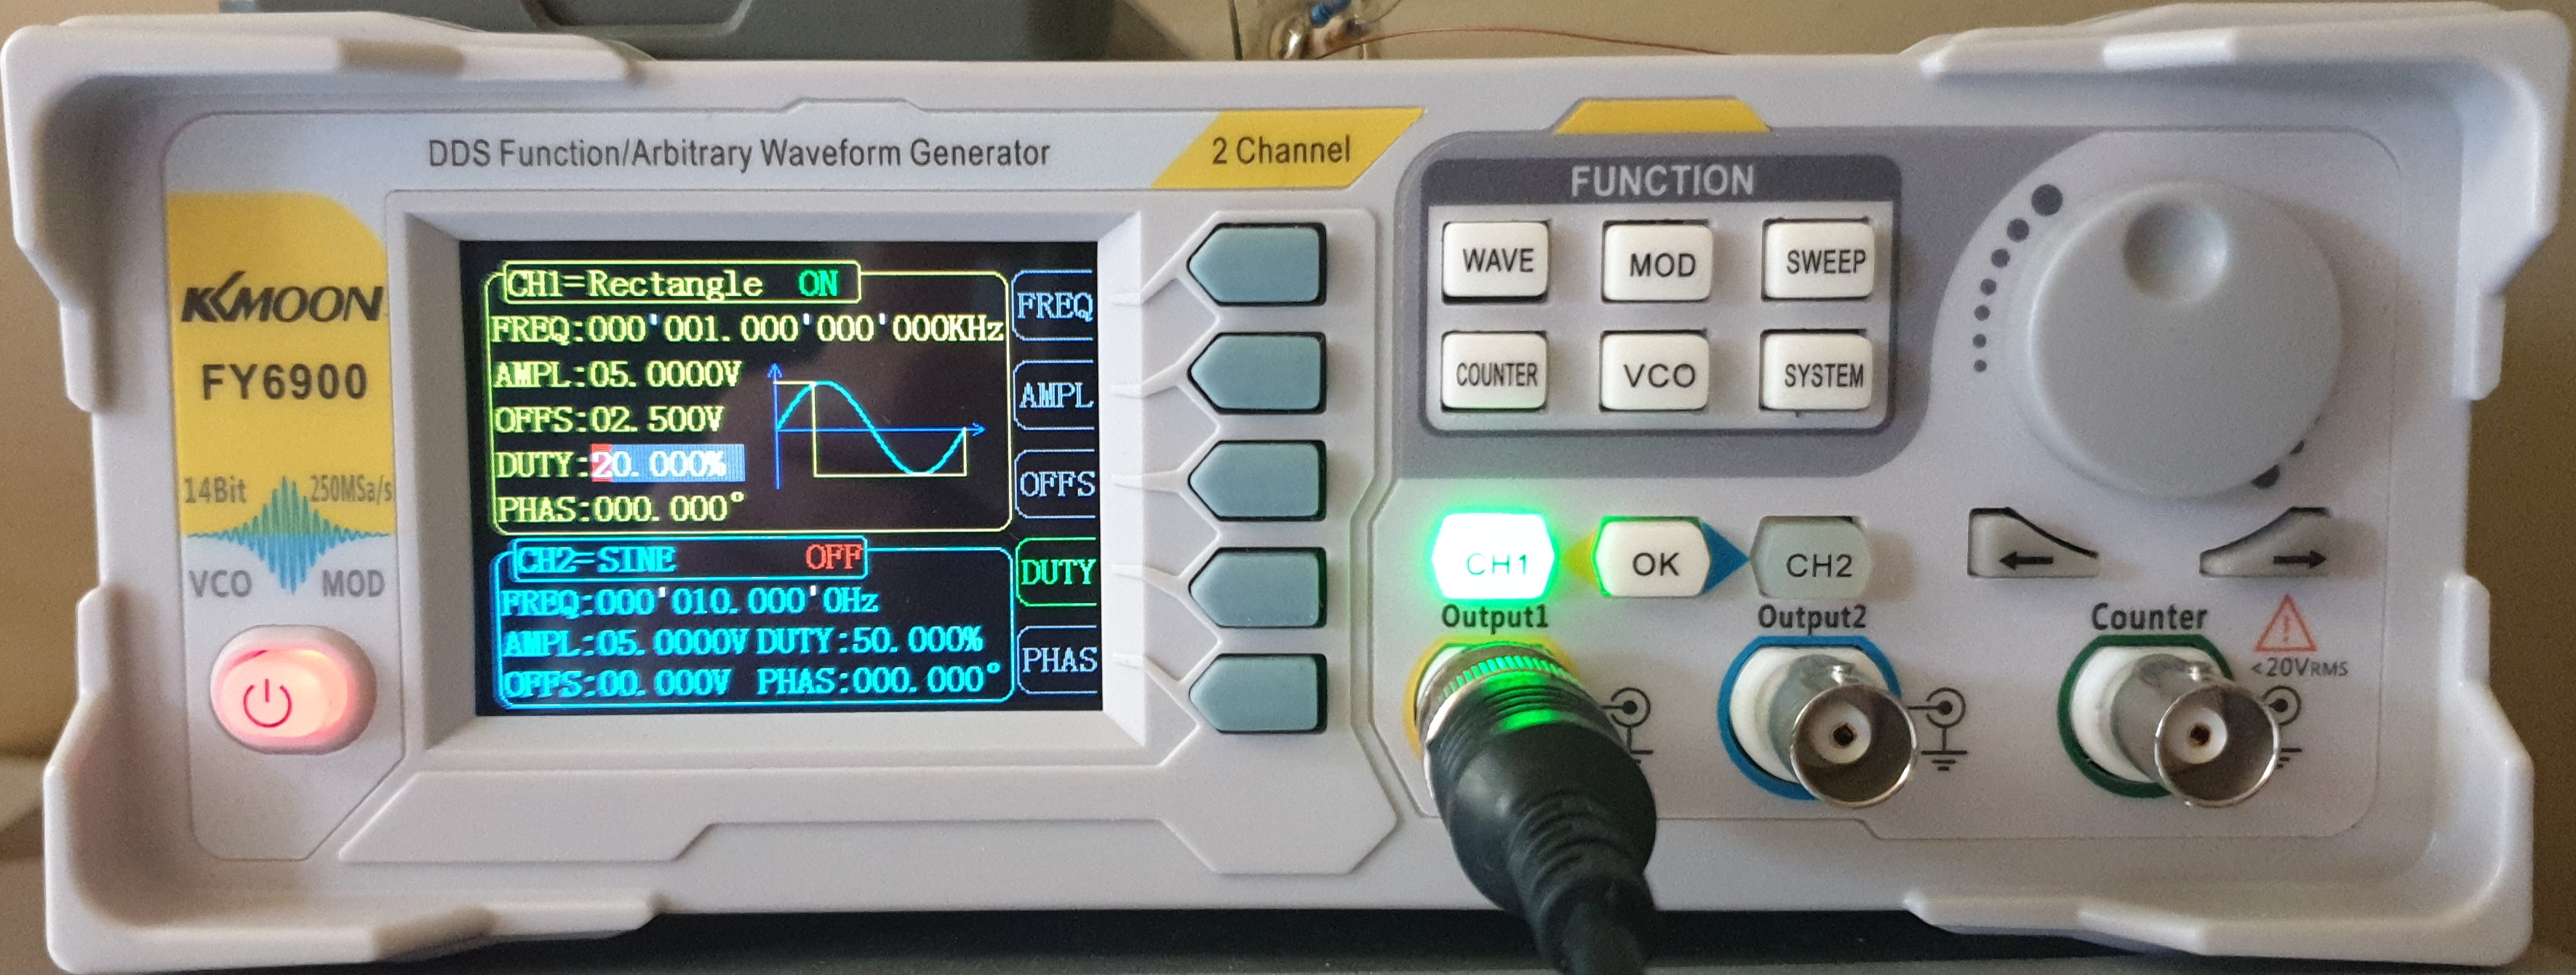
\includegraphics[width=0.90\textwidth]{ambient-linear-gen}
    \\ \vspace{5mm}
    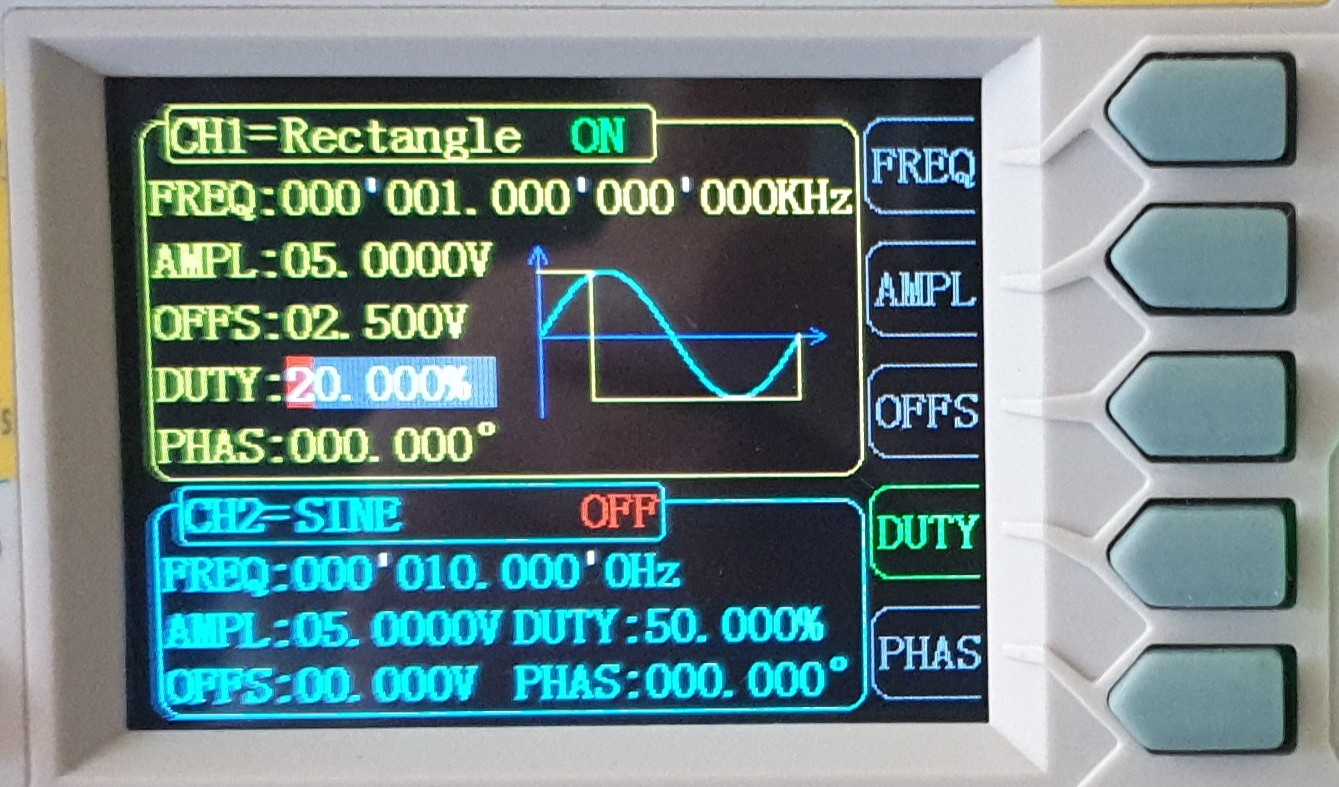
\includegraphics[height=4.5cm]{ambient-linear-gen-ch1}
    \hfill
    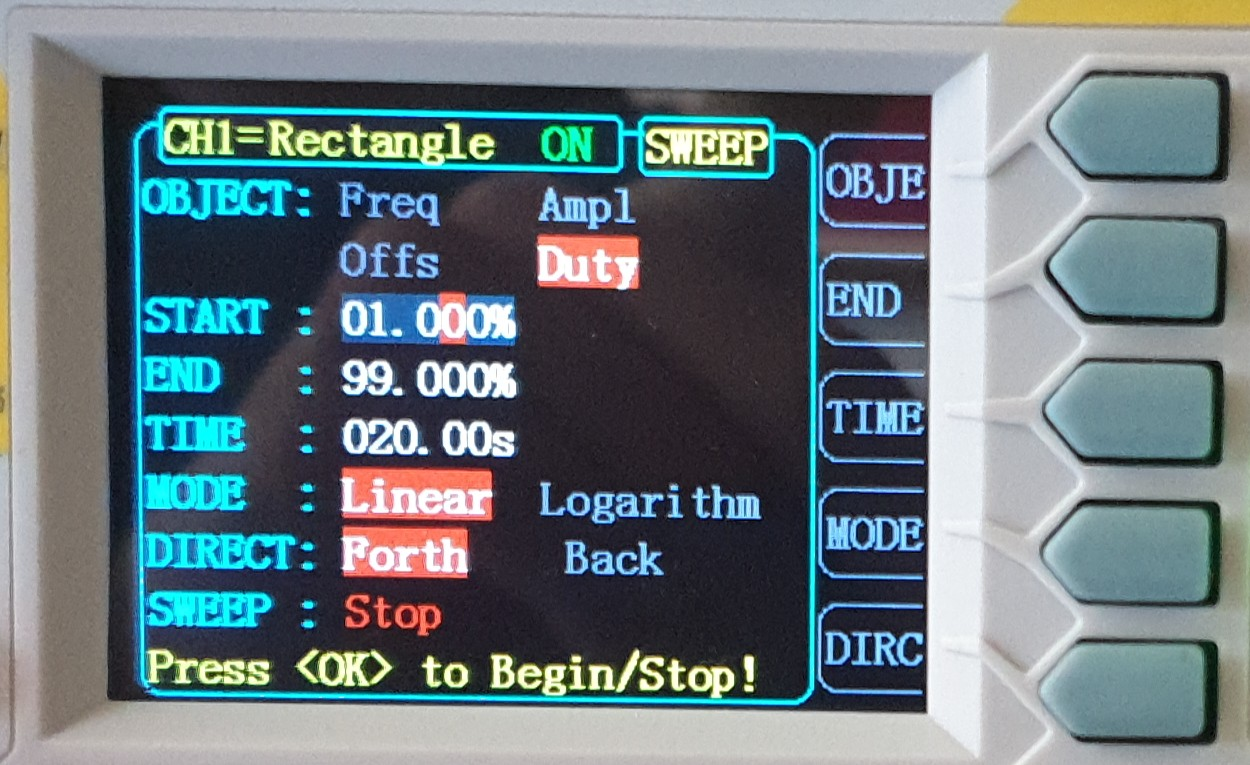
\includegraphics[height=4.5cm]{ambient-linear-gen-sweep}
    \caption{%
        Nastavení generátoru funkcí FY6900 pro měření charakteristiky stmívače
    }
    \label{fig:ambient linear mereni generator}
\end{figure}

K~testovanému obvodu je připojen digitální osciloskop Agilent~54621A, kterým je
měřeno napětí na rezistoru R4, které je přímo úměrné proudu protékajícímu LED
diodou (proud protékající bází Q3 můžeme zanedbat). Časová základna osciloskopu
je nastavena na \SI{2}{\second}/dílek, režim spouště \texttt{NORMAL}, spouštění
na sestupné hraně použitého vstupního kanálu (na následujících snímcích
obrazovky je to kanál 2) a~posunutí okamžiku spuštění k~levému okraji
obrazovky. Na obrazovce osciloskopu je tedy zobrazen celý průběh
charakteristiky. Od sestupné hrany signálu střída lineárně narůstá od
\SI{1}{\percent} do \SI{99}{\percent}, lze ji proto považovat za veličinu
vynášenou na vodorovné ose.

Osciloskop umožňuje uložení úplného nastavení do textového souboru na disketu:
\begin{lstlisting}[style=terminal]
Anlg Ch State  Units/Div  Position  Coupling  BW Limit  Invert
 Ch 2:    On     200mV/     600mV      DC        Off      Off

Anlg Ch Impedance   Probe
 Ch 2:    1M Ohm   1.0 : 1

Trigger  Mode   Coupling  Noise Rej  HF Reject  Holdoff
  Edge  Normal     DC         On         On       60ns

Trigger Source   Slope    Level
         Ch 2   Falling  +391mV

Time Time Ref  Main s/div  Delay
Main   Left      2.00s/     0.0s

Acquisition Realtime  Vectors  Infinite Persistence
   Normal      Off       On             Off
\end{lstlisting}

Pro porovnávání průběhů charakteristiky na obrazovce digitálního osciloskopu
lze využít funkci uložení referenčního průběhu. Ten je na obrazovce zobrazen
světlejší barvou.

Na obrázku~\vref{fig:ambient linear mereni scope dioda} jsou zobrazeny dvě
charakteristiky. Světlejší z~nich je uložený referenční průběh, který byl
změřen na obvodu, ve kterém byl emitor Q1 přímo spojený se zemí. Tmavší průběh
byl změřen po zařazení diody. Pozorujeme, že dochází ke zvětšení rozsahu
regulace a~prodloužení lineární části charakteristiky.

\begin{figure}[htbp]
    \centering
    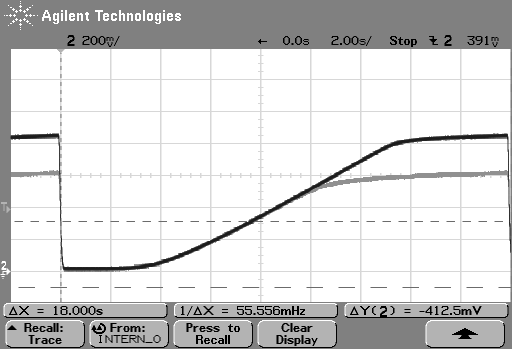
\includegraphics[width=0.80\textwidth]{scope-ambient-linear-diode}
    \caption{%
        Vliv diody připojené v~propustném směru v~emitoru Q1 na chování
        lineárního stmívače
    }
    \label{fig:ambient linear mereni scope dioda}
\end{figure}

\begin{figure}[htbp]
    \centering
    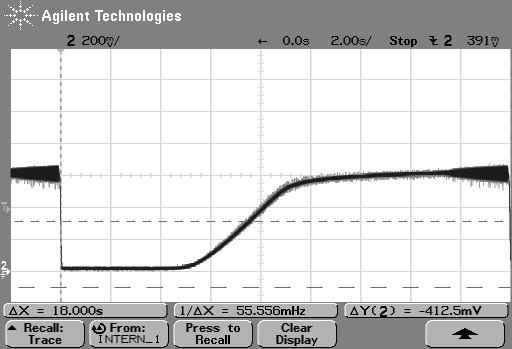
\includegraphics[width=0.80\textwidth]{scope-ambient-linear-oscillations}
    \caption{%
        Charakteristika lineárního stmívače s~nevhodným průběhem a~viditelnými
        oscilacemi
    }
    \label{fig:ambient linear mereni scope oscilace}
\end{figure}


% Schema z KiCAD. Zatim ho sem davat nebudu, melo by jine refdes apod.
%\begin{figure}[htbp]
%    \centering
%    %\includegraphics[width=0.9\textwidth]{cropped_ambient-linear-prod}
%    \caption{%
%        Schéma zapojení konečné verze lineárního stmívače pro výkonovou LED}
%    \label{fig:ambient linear prod sch}
%\end{figure}

\section{Indikace výpadku napájení}
Protože je budík napájen stejnosměrným napětím \SI{5}{\volt} získaným ze zdroje
závislého na síti, může dojít k~nečekanému výpadku napájení. V~takovém případě
musí budík selhat bezpečně. Bezpečným selháním je okamžité vzbuzení uživatele,
aby nemohlo při dlouho trvajícím výpadku dojít k~jeho zaspání. Tento přístup
byl zvolen, protože zajištění plné funkce při výpadku napájení by vyžadovalo
přidání akumulátoru a~složitých nabíjecích obvodů.

\begin{figure}
    \centering
    \includegraphics[page=1, clip, bb=90mm 12mm 176mm 58mm, width=0.80\textwidth]{prilohy/AlarmClock-hardware/AlarmClock/AlarmClock.pdf}
    \par\bigskip
    \caption{Schéma zapojení obvodu akustické indikace výpadku napájení}
    \label{fig:UPS sch}
\end{figure}

Pro akustickou indikaci je využit aktivní bzučák, tedy piezoelektrický měnič
s~interním generátorem budicího signálu. Pro jeho provoz je nutné pouze
stejnosměrné napájecí napětí (jmenovitá hodnota je \SI{3,3}{\volt}).
Jako zdroj energie pro bzučák je použita knoflíková baterie typu CR2032, která
slouží i~jako záložní baterie hodin reálného času. Protože jde o~primární
lithiový článek, je nutné minimalizovat proudový odběr v~obou klidových
stavech (připojené napájení s~plnou funkčností budíku a~odpojené napájení po
zaznění zvukového signálu). V~době výpadku již neběží na \acs{MCU} program,
proto je nutné implementovat funkčnost akustické indikace v~hardware.

Obvod je navržen tak, že pokud je připojené napájení \SI{5}{\volt} a~na vstupu
\texttt{buzzer} je napětí \SI{5}{\volt}, bzučák nepíská. Pokud je připojeno
napájení, ale vstup \texttt{buzzer} je připojen k~zemi či zcela odpojen, píská
bzučák nepřetržitě. Pokud dojde k~výpadku napájení, neprotéká diodou ze vstupu
\texttt{buzzer} žádný proud a~bzučák píská, dokud nedojde k~vybití
elektrolytického kondenzátoru v~RC článku a~zavření NPN tranzistoru (doba
pískání je přibližně \SI{3}{\second}). Rezistor s~odporem \SI{100}{\kilo\ohm}
připojený paralelně ke kondenzátoru zajišťuje rychlejší vybíjení v~okolí
prahového napětí přechodu báze--emitor NPN tranzistoru, který se díky tomu
rychleji zavře.

Protože je v~obvodu zahrnuta nelineární součástka (přechod báze--emitor NPN
tranzistoru), nelze napětí na vybíjejícím se kondenzátoru matematicky modelovat
jednoduchou klesající exponenciálou. Lze ale využít simulátor elektronických
obvodů (viz obrázek~\vref{fig:UPS RC sim}). Výpadek napájení je simulován
pomocí direktivy \verb|.ic|, která určuje počáteční podmínky simulace. Napětí
na kondenzátoru je v~čase $t=0$ nastaveno na \SI{4,4}{\volt} (\SI{5}{\volt}
mínus úbytek napětí na křemíkové diodě).
% - vybijeni kondiku z (5V-0.6V) na 0.6V zabere 2tau
%   gnuplot> plot [0:5] 4.4*(exp(-x)), 0.6

\begin{figure}
    \centering
    \subcaptionbox{%
        Schéma zapojení a~nastavení simulace%
        \label{fig:UPS RC sim sch}
    }{%
        \includegraphics[width=0.7\textwidth]{sim/cropped_vypadek-RC}%
    }
    \subcaptionbox{%
        Časový průběh proudu protékajícího rezistorem $R_3$ po výpadku
        napájení%
        \label{fig:UPS RC sim proud}
    }{%
        \input{sim/graf-vypadek-RC.tex}%
    }
    \par\bigskip
    {\footnotesize Označení součástek neodpovídá schématu na
    obrázku~\vref{fig:UPS sch}}
    \caption{%
        Simulace časovacího obvodu indikátoru výpadku napájení v~programu
        LTspice
    }
    \label{fig:UPS RC sim}
\end{figure}

Připojením vstupu \texttt{buzzer} na výstupní pin MCU můžeme zajistit, že
bzučák reaguje například i~na vyjmutí MCU z~patice či běh nesprávného programu,
který na tento výstup nenastavuje logickou 1.

Praktickým měřením bylo ověřeno, že proud protékající diodou v~závěrném směru
(D1 na obrázku~\vref{fig:UPS sch}) nestačí ani po zesílení PNP tranzistorem Q2
pro znatelné zvýšení rychlosti vybíjení baterie BT1.

\FloatBarrier % TODO global?
\section{Proces návrhu a výroby desky plošných spojů}
\subsection{Návrh DPS}
Pro návrh DPS byl využit svobodný software KiCAD. Součástky a jejich propojení
jsou importovány ze schématu, jejich rozmístění na DPS a propojení cestami ale
musí provést člověk.

Před generováním návrhu plošného spoje je vhodné ověřit správnost schématu
nástrojem ERC (Electrical Rules Checker).

\begin{figure}[htbp]
    \centering
    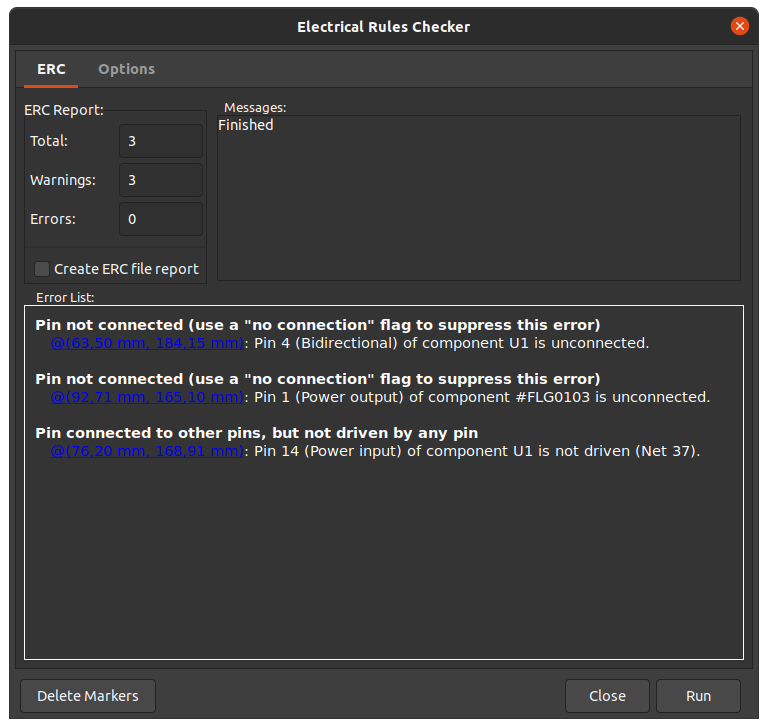
\includegraphics[width=0.70\textwidth]{KICAD-ERC}
    \caption{Výsledek kontroly ERC s několika detekovanými chybami}
    \label{fig:kicad ERC}
\end{figure}

\begin{figure}[htbp]
    \centering
    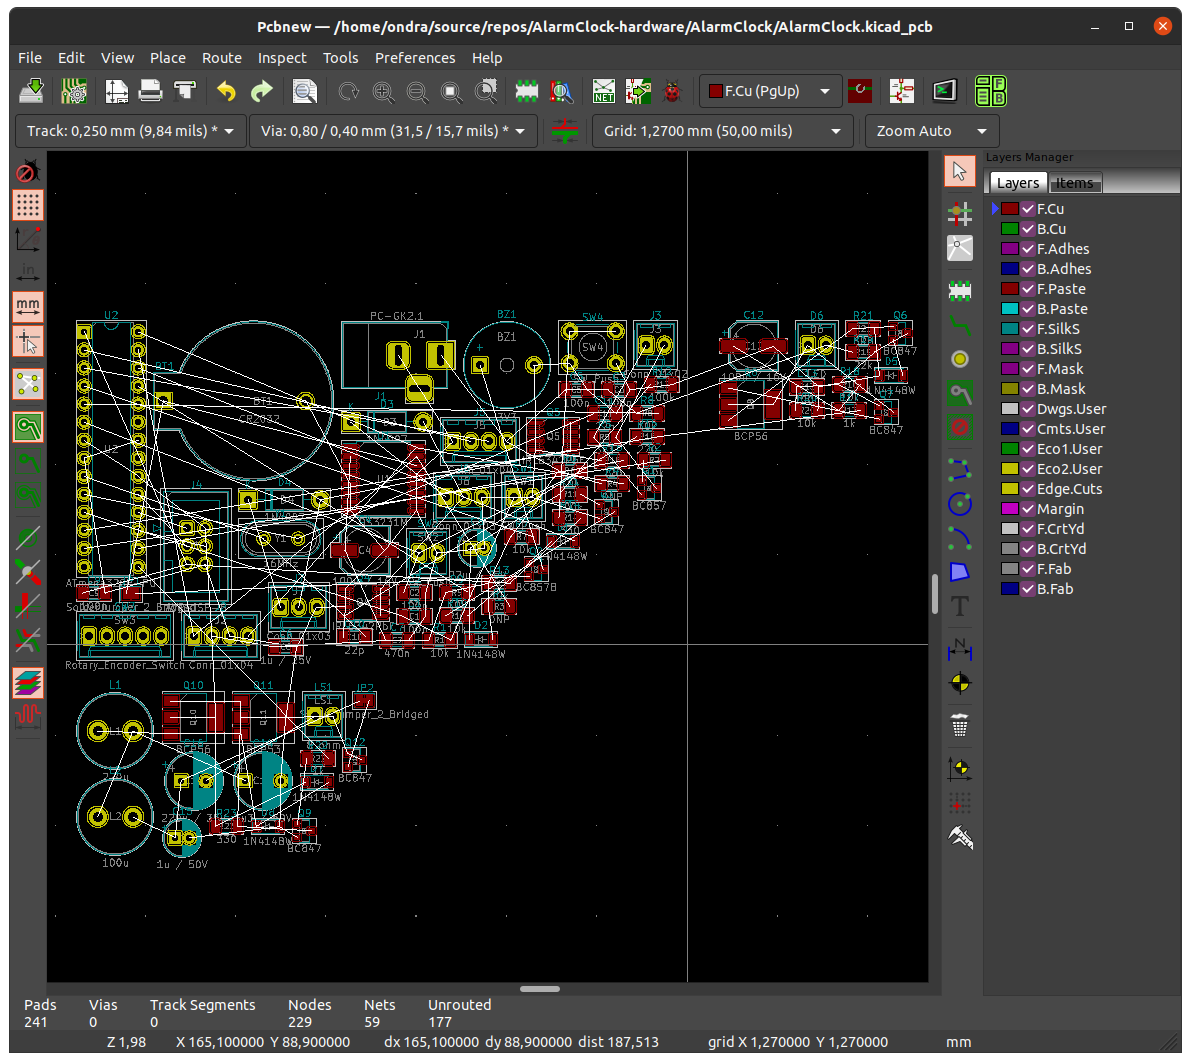
\includegraphics[width=0.80\textwidth]{KICAD-po-importu}
    \caption{%
        Nástroj pro návrh DPS \shellcmd{pcbnew} po importu součástek ze
        schématu
    }
    \label{fig:kicad po importu}
\end{figure}

Nástroj pro kontrolu správnosti návrhu plošného spoje se nazývá DRC. Ten
kontroluje, zda-li je možné DPS vyrobit procesem s definovanými vlastnostmi
(minimální šířka cesty, minimální izolační mezera, ...). Pro proces frézování
je vhodné používat poměrně široké cesty~-- \SI{1}{\milli\meter} pro většinu
spojů, \SI{0,8}{\milli\meter} pro cesty propojující SMD integrované obvody.

DPS byla navržena tak, aby ji bylo možné vyrobit s mědí z jedné strany či
oboustranně. Na jednostranném plošném spoji jsou cesty na horní měděné vrstvě
nahrazeny drátovými propojkami.

Úplné schéma zapojení a návrh DPS jsou otištěny v příloze~\ref{app:PCB}.


\subsection{Výroba DPS}
Pro výrobu prototypů desek plošných spojů lze využít metodu vytváření
izolačních mezer v měděné vrstvičce pomocí CNC frézy. Jde o poměrně rychlou
metodu s minimem manuální práce. Stroj navíc provádí i navrtání děr, jejichž
počet i na poměrně jednoduchých DPS využívajících v maximální možné míře
součástek pro povrchovou montáž dosahuje několika stovek. Celý proces se obejde
bez nutnosti pracovat s korozivními chemikáliemi. Frézování oboustranných DPS
je možné, v takovém případě se ale zvyšuje náročnost postupu. Je totiž nutné
zachovat pozici referenčního bodu při otáčení desky.

\subsubsection{CNC fréza}
Levným CNC strojem splňujícím požadavky na přesnost, rozměry pracovního
prostoru a podporované funkce vhodným pro amatérské účely je stavebnice
prodávaná prodejci na platformě Aliexpress pod označením CNC~1610. Je tvořena
konstrukcí z hliníkových profilů a několika 3D tištěných částí. Po sestavení
získává uživatel stroj s pracovním prostorem \SI{160 x 100 x 40}{\milli\meter}
řízený svobodným firmware Grbl\footnote{\url{https://github.com/gnea/grbl}}.

\begin{figure}[htbp]
    \centering
    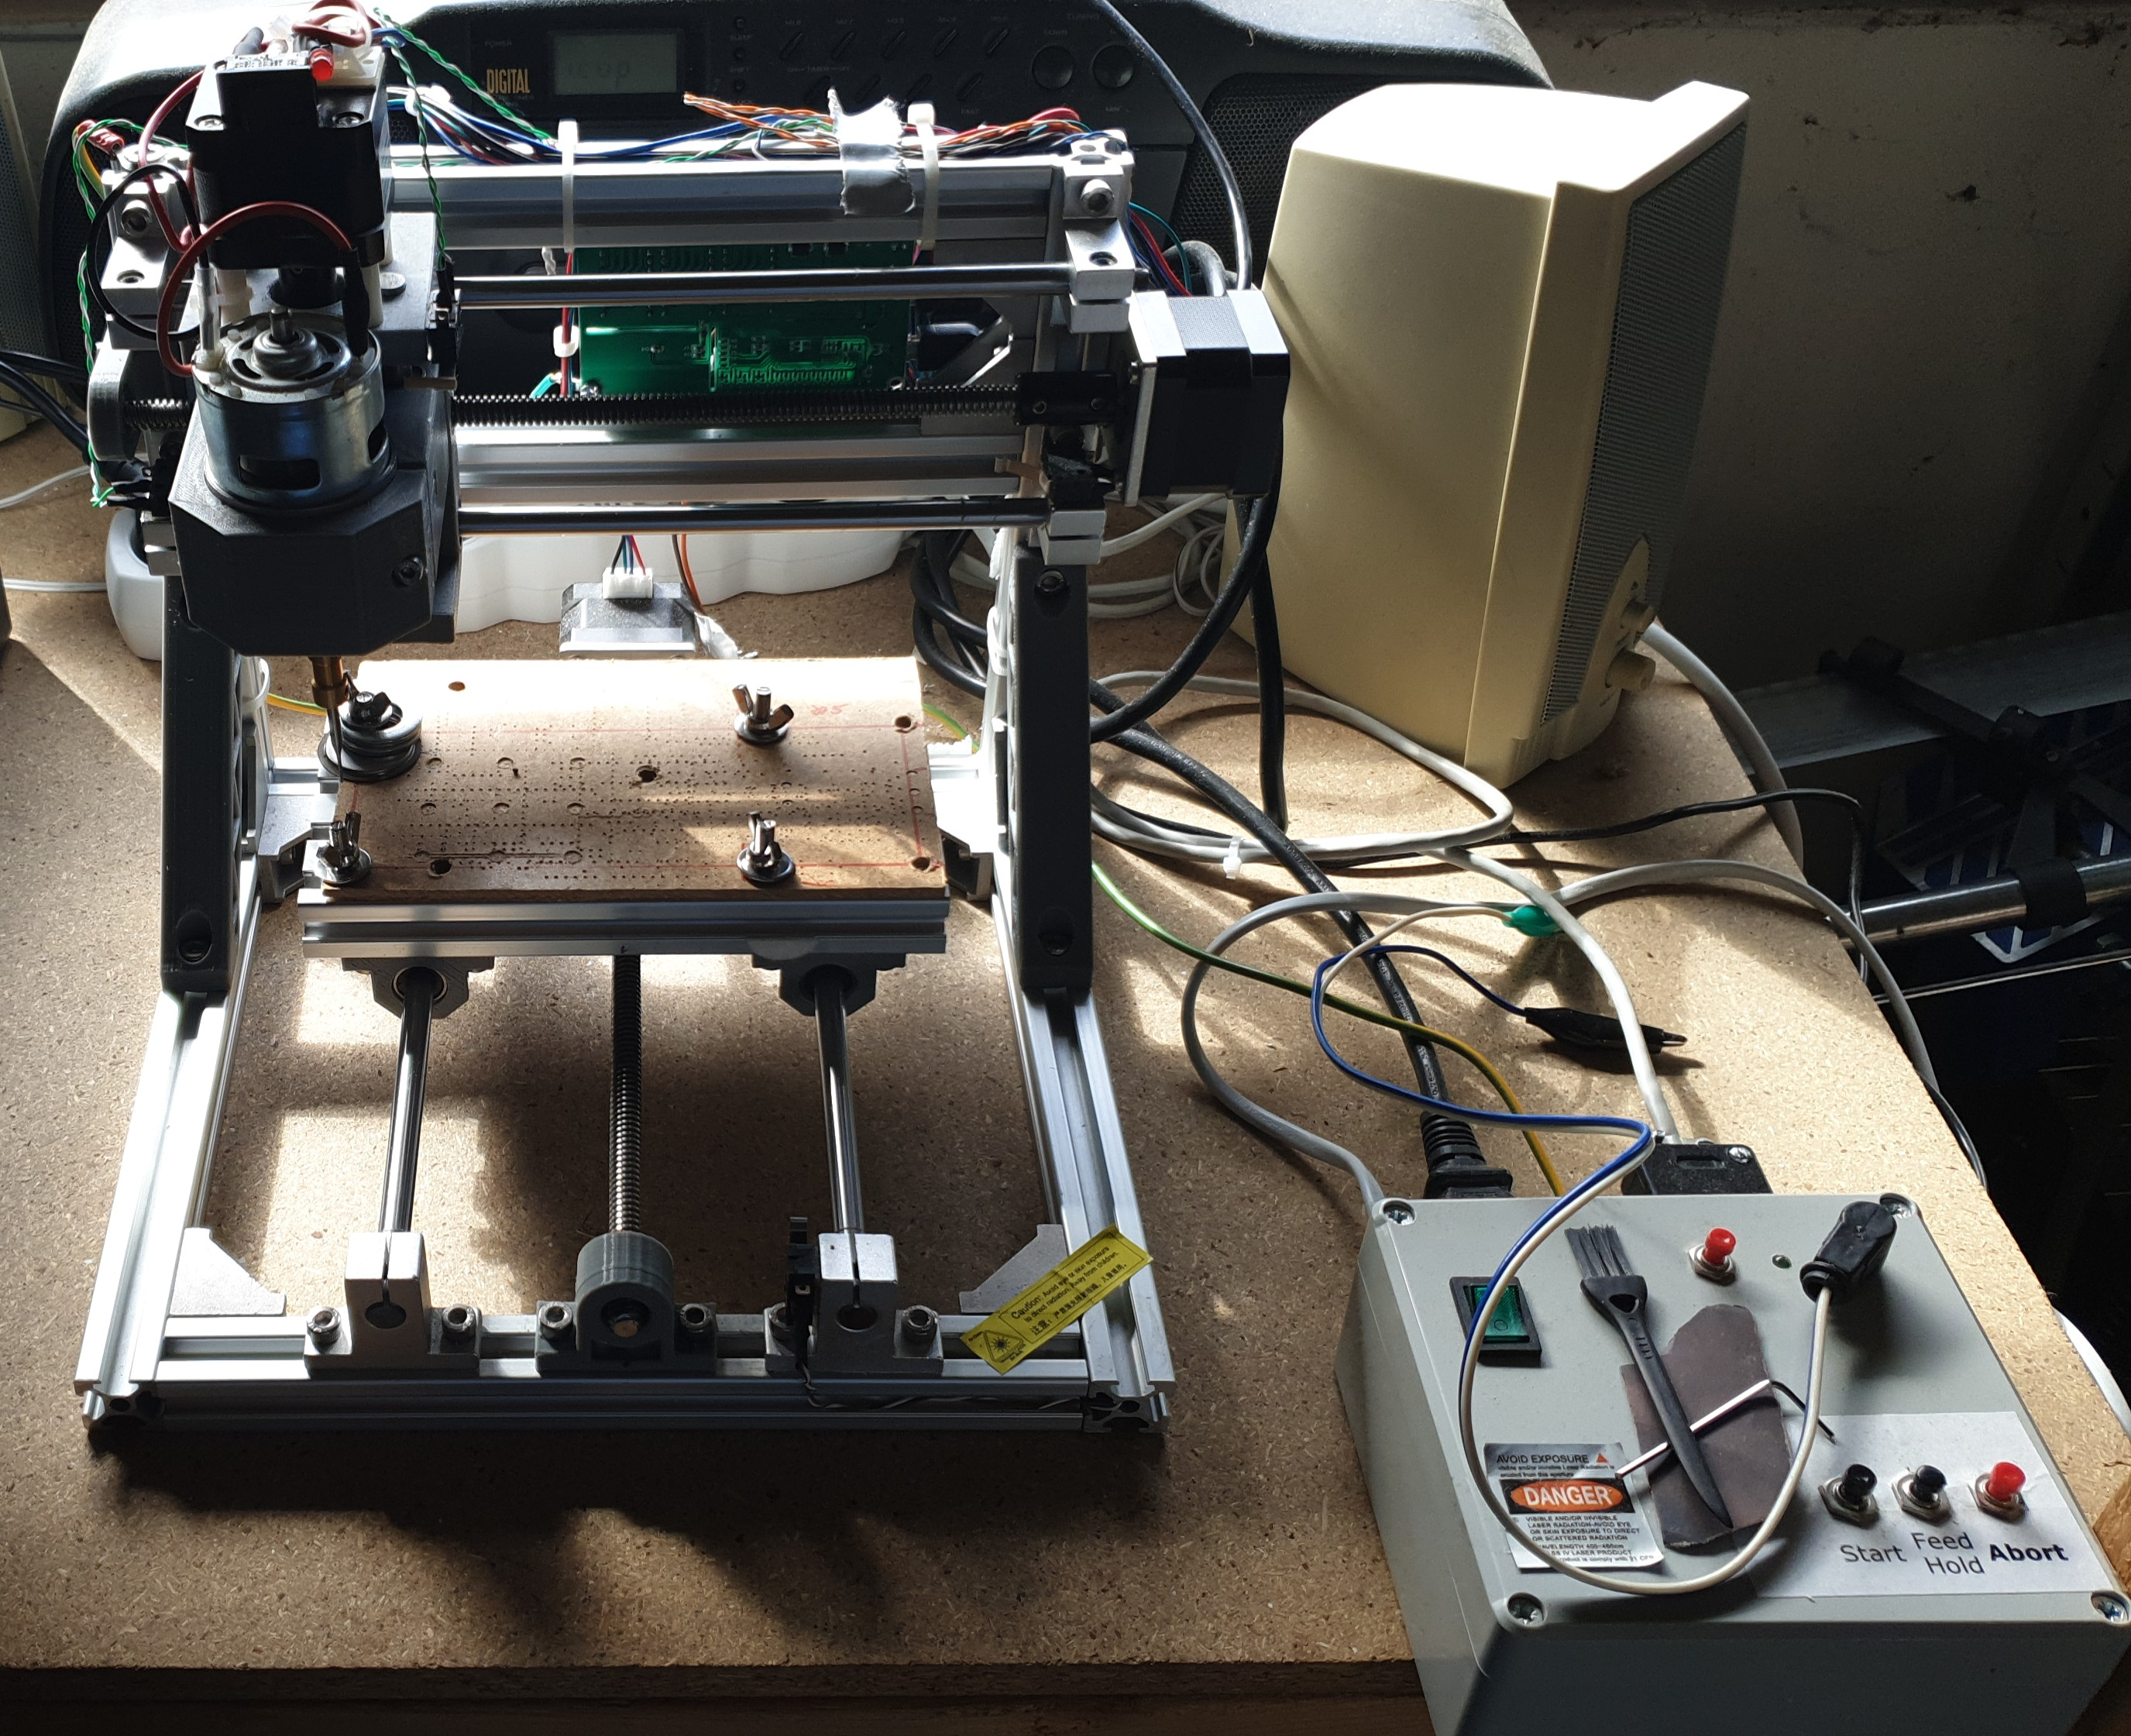
\includegraphics[width=1.0\textwidth]{CNC-freza}
    \caption{CNC fréza CNC~1610 s drobnými úpravami}
    \label{fig:CNC freza}
\end{figure}


\paragraph{Modifikace}
Po zakoupení stroje byly provedeny některé modifikace, které nadále
zjednodušují proces výroby DPS. Jednou z nich je přidání koncových spínačů.
Jejich funkce je dvojí. Zvyšují bezpečnost, protože zabraňují nárazu
pohyblivých částí stroje do jeho rámu (v případě využití
\foreignlanguage{english}{homing cycle} dokonce nemusí nutně dojít ani
k sepnutí tohoto spínače, pohyb mimo pracovní prostor je detekován výpočetně).
Umožňují také provést po spuštění stroje kalibraci
(\foreignlanguage{english}{homing cycle}), po které odpovídají souřadnice
stroje (v Grbl zvané \foreignlanguage{english}{machine coordinates})
konkrétním bodům v jeho pracovním prostoru. Díky tomu je možné beze ztráty
přesnosti obnovit práci například po výpadku napájení.

Druhá modifikace je pro výrobu DPS ještě důležitější. Jde o přidání kabelů
s krokosvorkami na vstup pro sondu (\foreignlanguage{english}{probe}). Jedna ze
svorek je spojena s měděnou vrstvou obráběné DPS, druhá je připojena na
frézovací nástroj upnutý v zastaveném vřetenu. Stroj díku tomu může přesně
změřit výšku desky v různých bodech a kompenzovat tak její průhyby. Vlastní
frézování je totiž velmi mělké, méně než \SI{200}{\micro\meter}.

\begin{figure}[htbp]
    \centering
    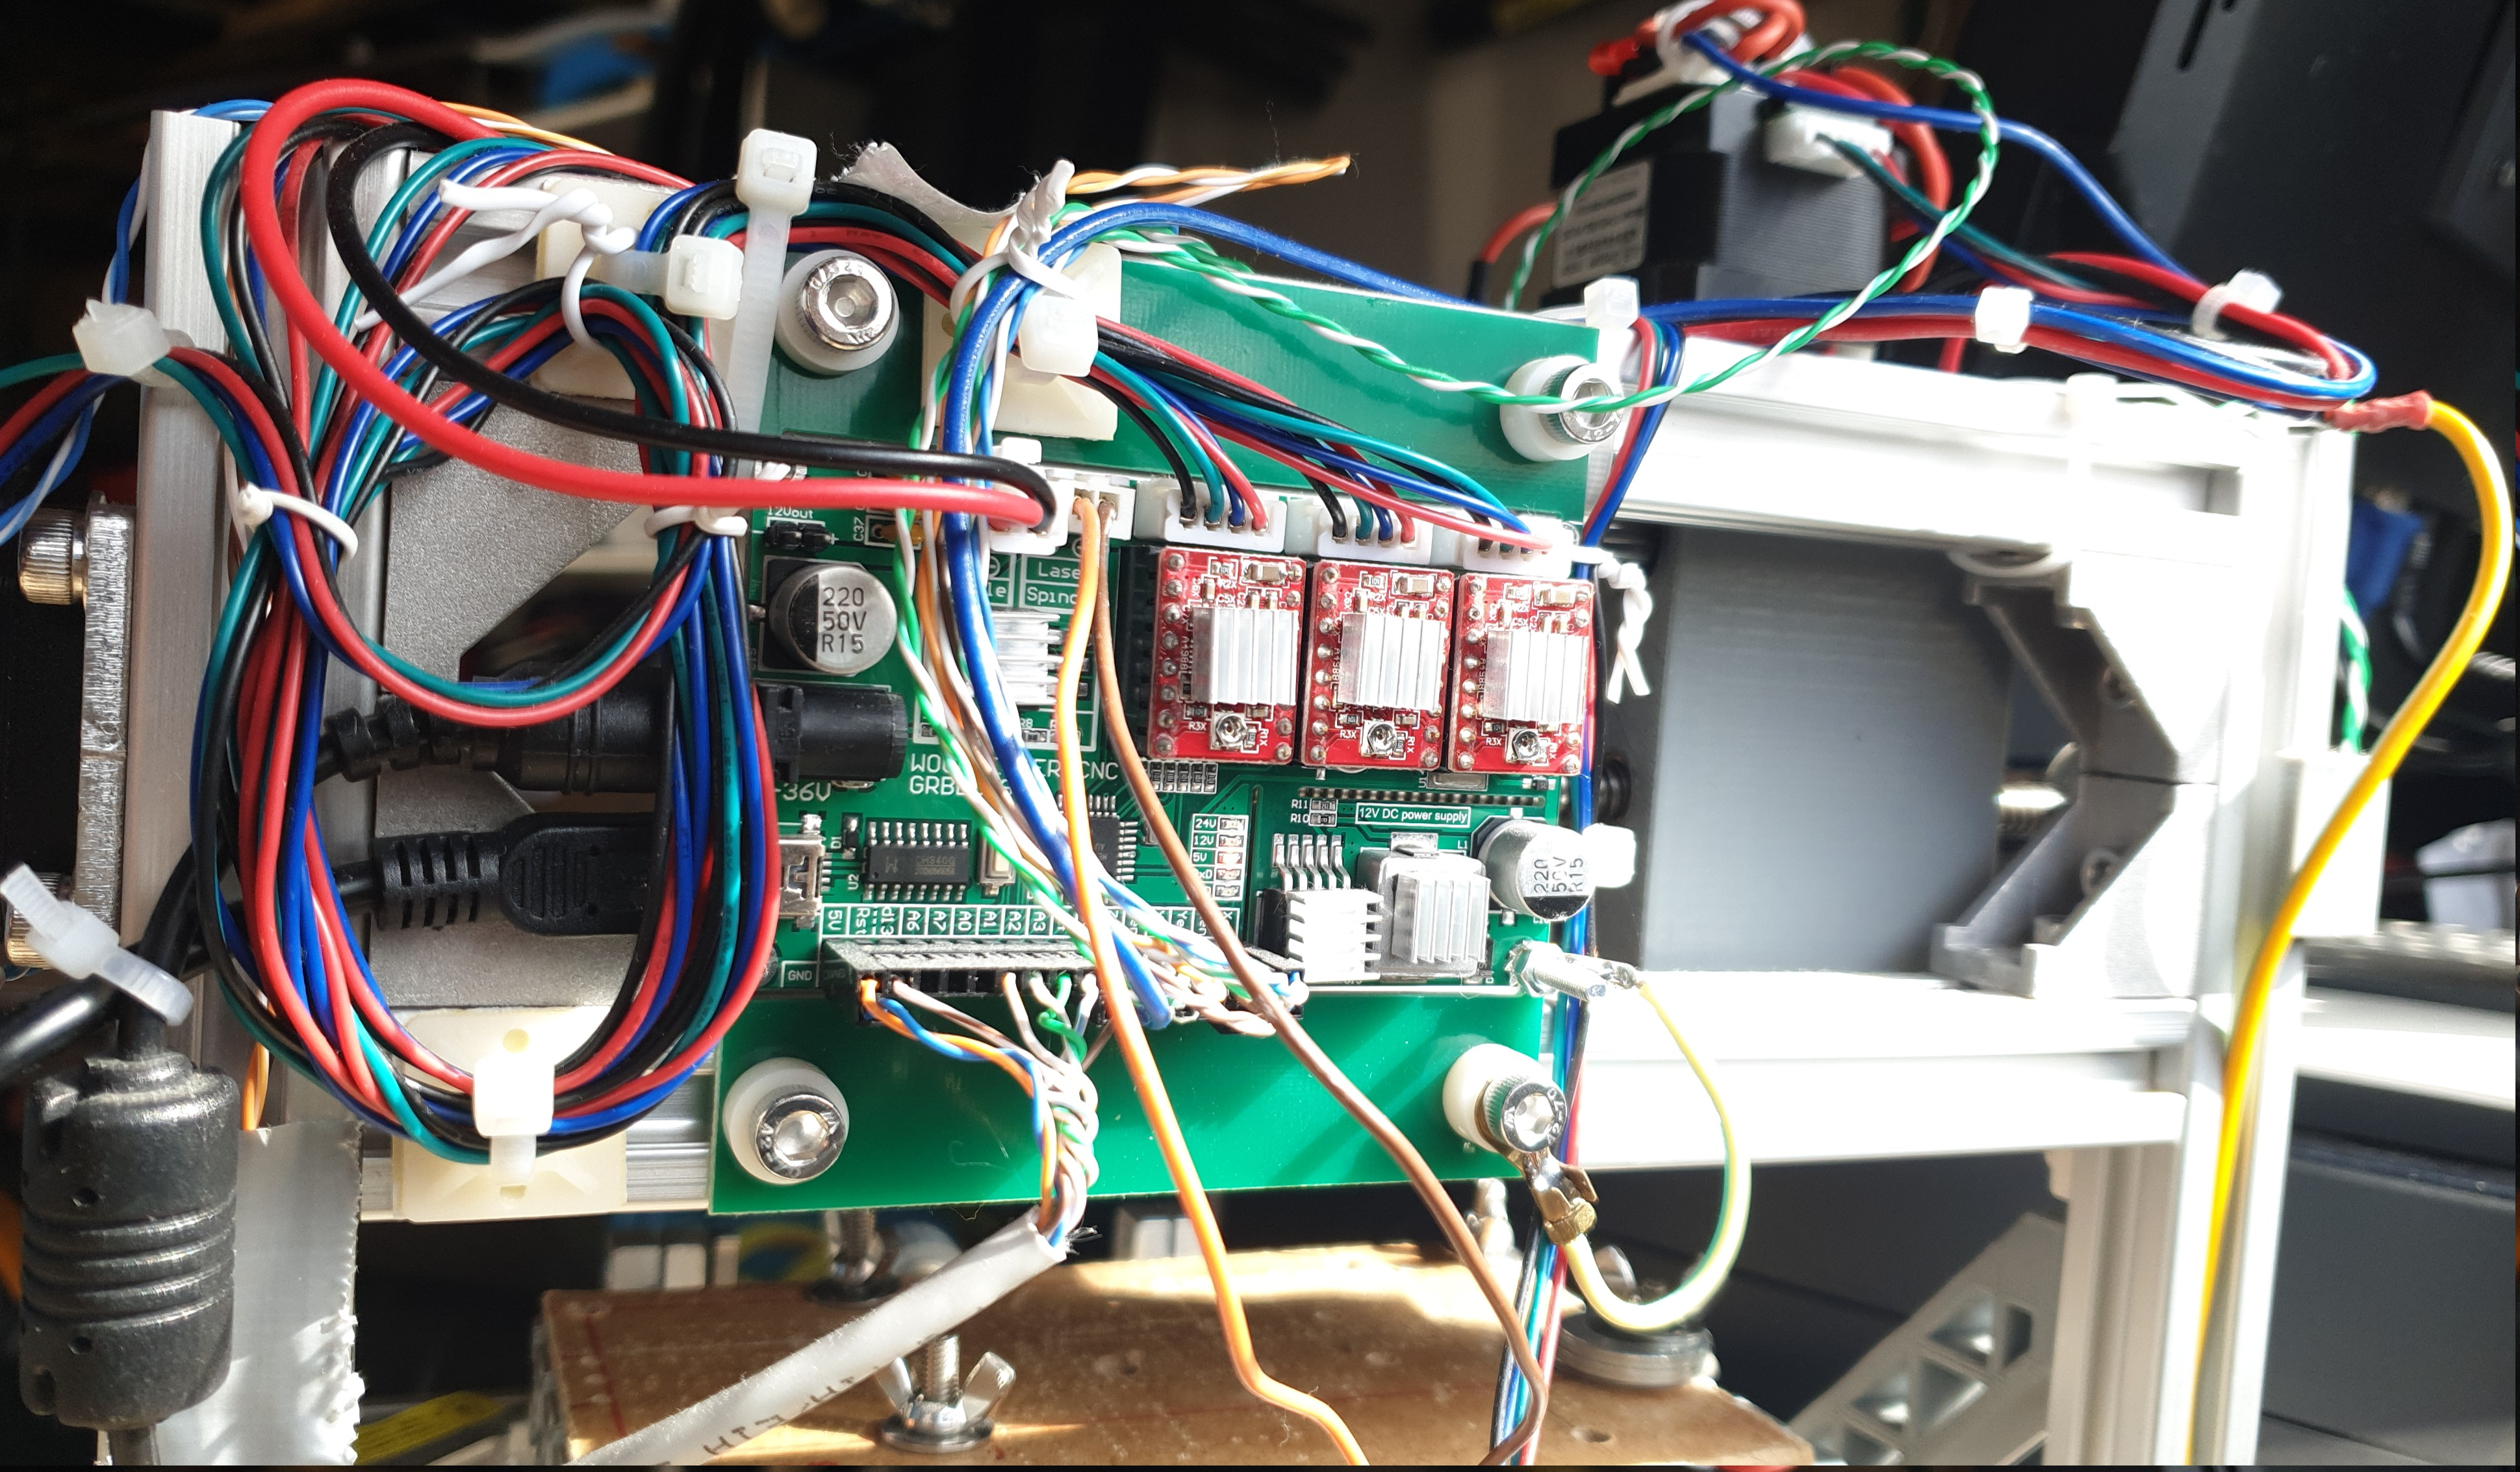
\includegraphics[width=1.0\textwidth]{CNC-rizeni}
    \caption{%
        Řídicí elektronika CNC frézy s připojenými koncovými spínači a~sondou
    }
    \label{fig:CNC rizeni}
\end{figure}

Po provedení modifikací je nutné správně změnit nastavení Grbl, zejména
\verb|$5|, \verb|$6|, \verb|$20|, \verb|$21| a \verb|$22| až \verb|$27|.
Je také nutné správně nastavit rozměry pracovního prostoru (\verb|$130| až
\verb|$132|), protože výrobce toto nastavení ignoruje a ponechává jej na
výchozí hodnotě. Úplná konfigurace Grbl včetně vysvětlení jednotlivých
nastavení je otištěna v příloze~\vref{app:grbl config}.

Aby bylo možné využívat novější verzi řídicího software (spouštěného na
počítači), je nutné aktualizovat firmware stroje z verze Grbl~0.9j na
Grbl~1.1h. Aktualizace se provádí dle instrukcí na domovské stránce projektu
Grbl pomocí Arduino IDE. Přečtením obsahu paměti FLASH s původním firmware bylo
zjištěno, že použitý bootloader odpovídá desce \uv{Arduino nano (old
bootloader)}. Před aktualizací je vhodné vytvořit zálohu původního obsahu
paměti. To lze na počítači s operačním systémem GNU/Linux s nainstalovaným
Arduino IDE provést následujícím příkazem:
\begin{lstlisting}[style=terminal]
$ $HOME/.arduino15/packages/arduino/tools/avrdude/6.3.0-arduino17/bin/avrdude \
    -C$HOME/.arduino15/packages/arduino/tools/avrdude/6.3.0-arduino17/etc/avrdude.conf \
    -v -patmega328p -carduino -P/dev/ttyUSB0 -b5 7600 -D \
    -Uflash:r:$HOME/Desktop/CNC/GRBL-old-read.bin:r
\end{lstlisting}
Dále je nutné zazálohovat nastavení Grbl, která jsou uložená v paměti EEPROM.
To se provádí připojením terminálu na sériový port stroje a spuštěním příkazu
\verb|$$|.
Po aktualizaci firmware je potřeba nová nastavení stroje porovnat s touto
zálohou a příslušně je upravit.

\paragraph{Nástroje}
Pro frézování obrazce DPS jsou vhodné nástroje ve tvaru V. Průměr nástroje
v místě upnutí je \SI{3,175}{\milli\meter}, to je standardní rozměr používaný
na malých CNC frézách. Nástroj se poté zužuje s úhlem
\SI{15}{\degree} až k velmi tenkému hrotu.

Pro vrtání děr využíváme tvrzené vrtáky o průměru \SI{0,8}{\milli\meter}
a \SI{1}{\milli\meter}. Tyto dva rozměry postačí pro naprostou většinu běžných
DPS. Montážní díry o průměru \SI{3,2}{\milli\meter} se tímto vrtákem předvrtají
a na požadovaný průměr je zvětšíme stojanovou vrtačkou. Drážky pro vývody
napájecího konektoru lze vyfrézovat frézou \uv{corn bit} o průměru
\SI{1}{\milli\meter}. Stejným nástrojem je provedeno i oddělení hotové DPS od
zbytku materiálu.

\begin{figure}[htbp]
    \centering
    \subcaptionbox{%
        V-bit a fréza \SI{1}{\milli\meter}
    }[0.3\textwidth]{%
        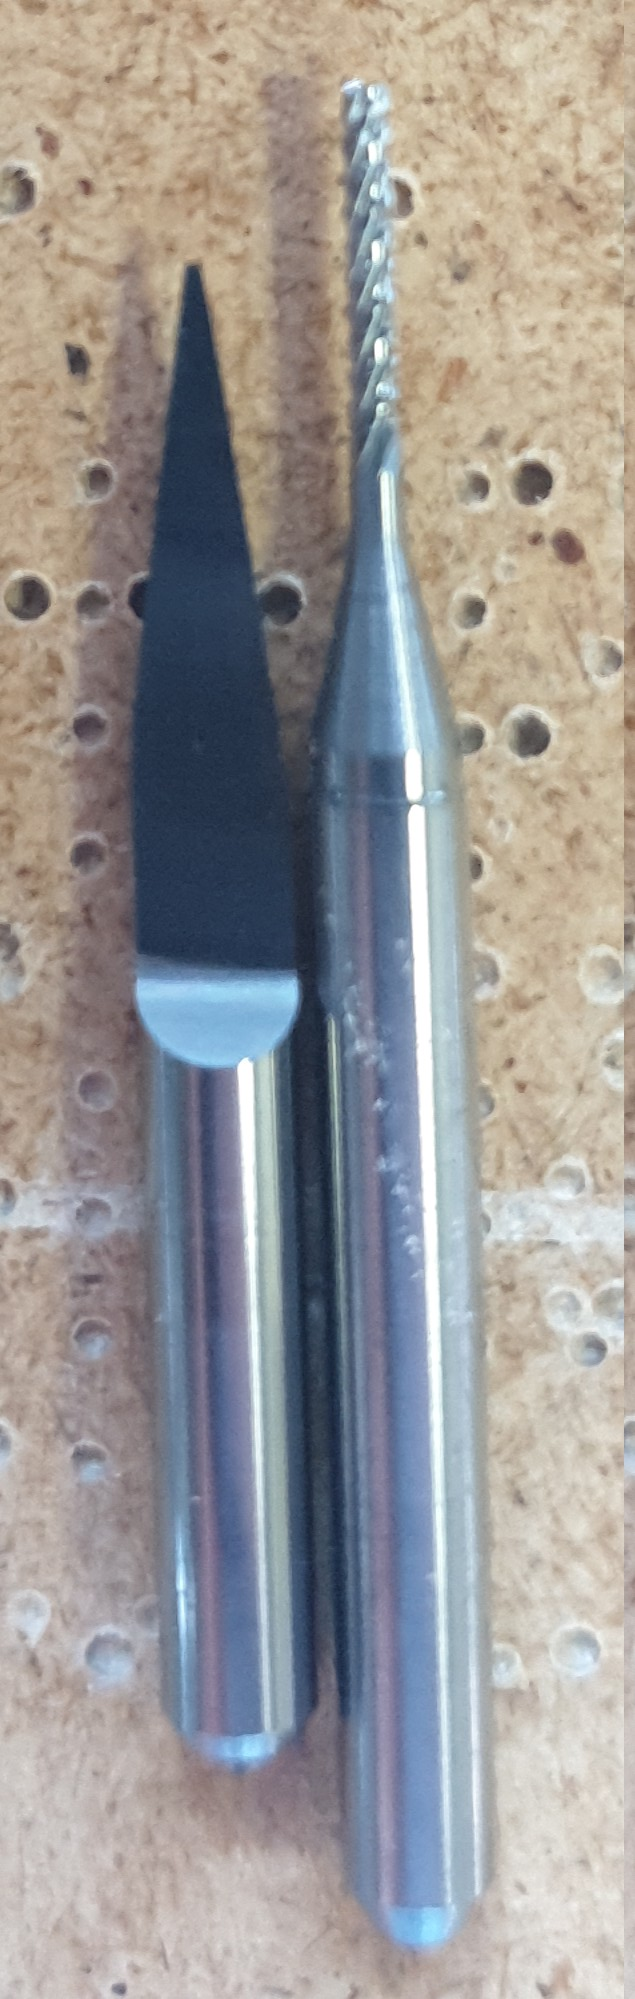
\includegraphics[height=50mm]{CNC-nastroj-V-freza}
    }
    \subcaptionbox{%
        Vrták \SI{0,8}{\milli\meter}
    }[0.3\textwidth]{%
        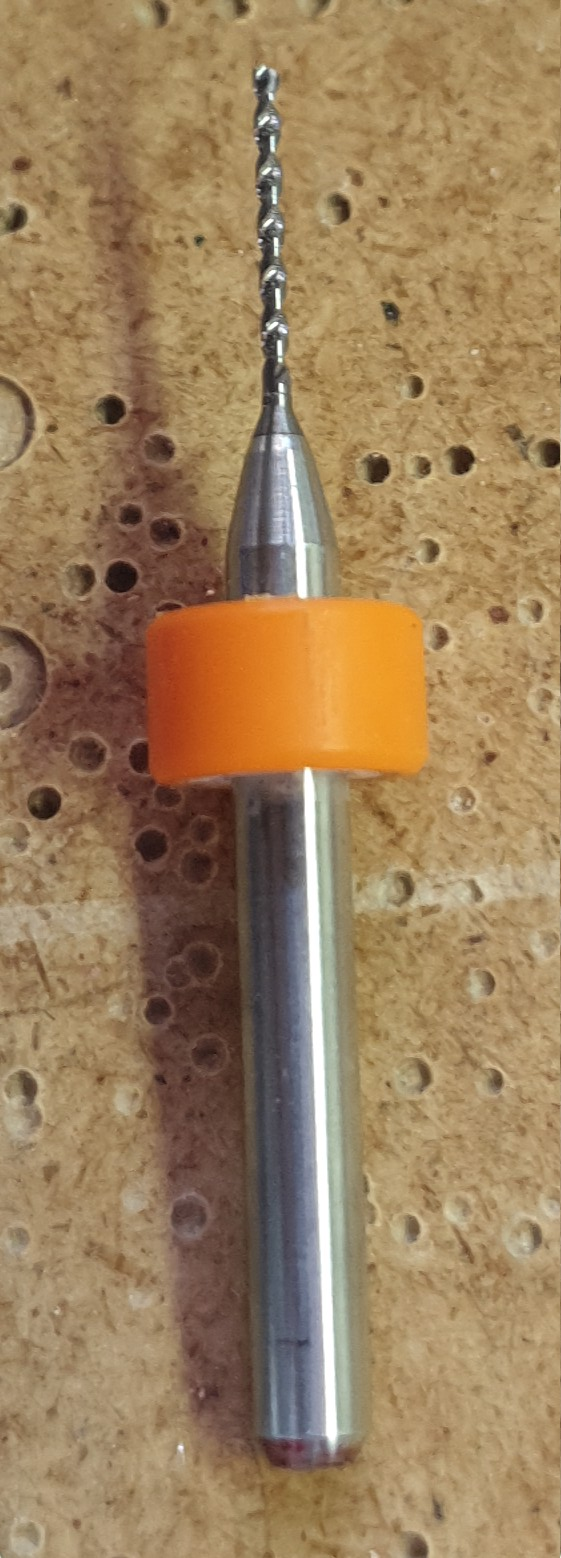
\includegraphics[height=50mm]{CNC-nastroj-08}
    }
    \subcaptionbox{%
        Vrták \SI{1,0}{\milli\meter}
    }[0.3\textwidth]{%
        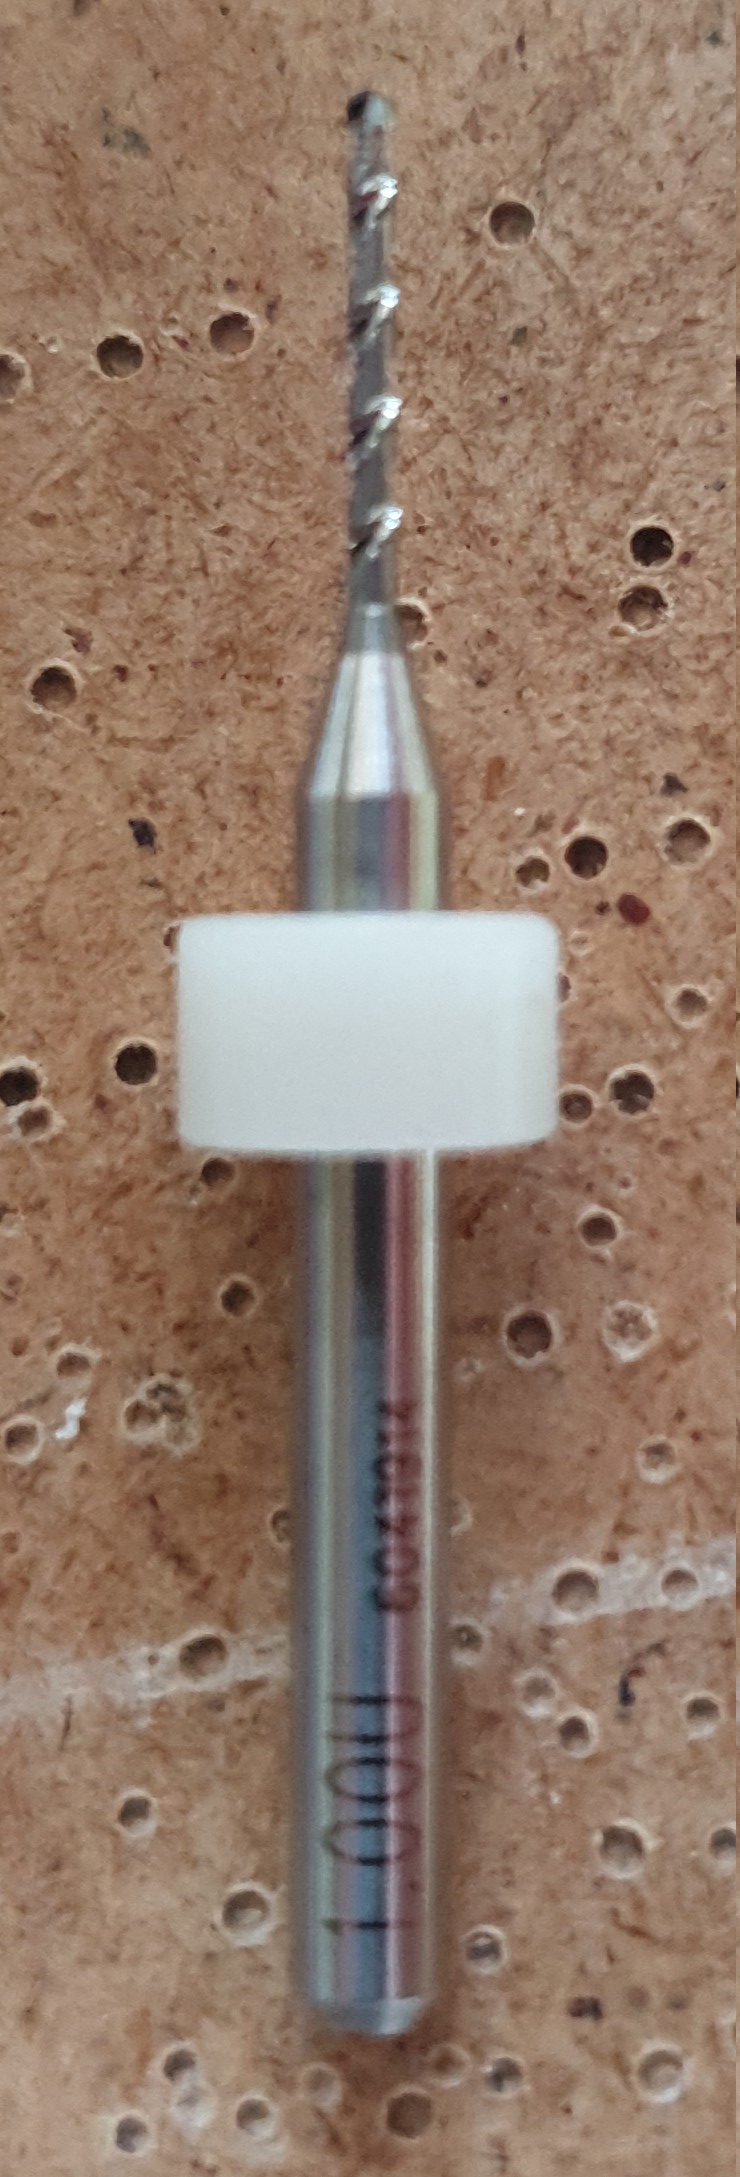
\includegraphics[height=50mm]{CNC-nastroj-10}
    }
    \caption{Nástroje používané při frézování DPS}
    \label{fig:CNC nastroje}
\end{figure}

\begin{figure}[htbp]
    \centering
    \includegraphics[width=0.65\textwidth]{CNC-drazky-nastroj}
    \hfill
    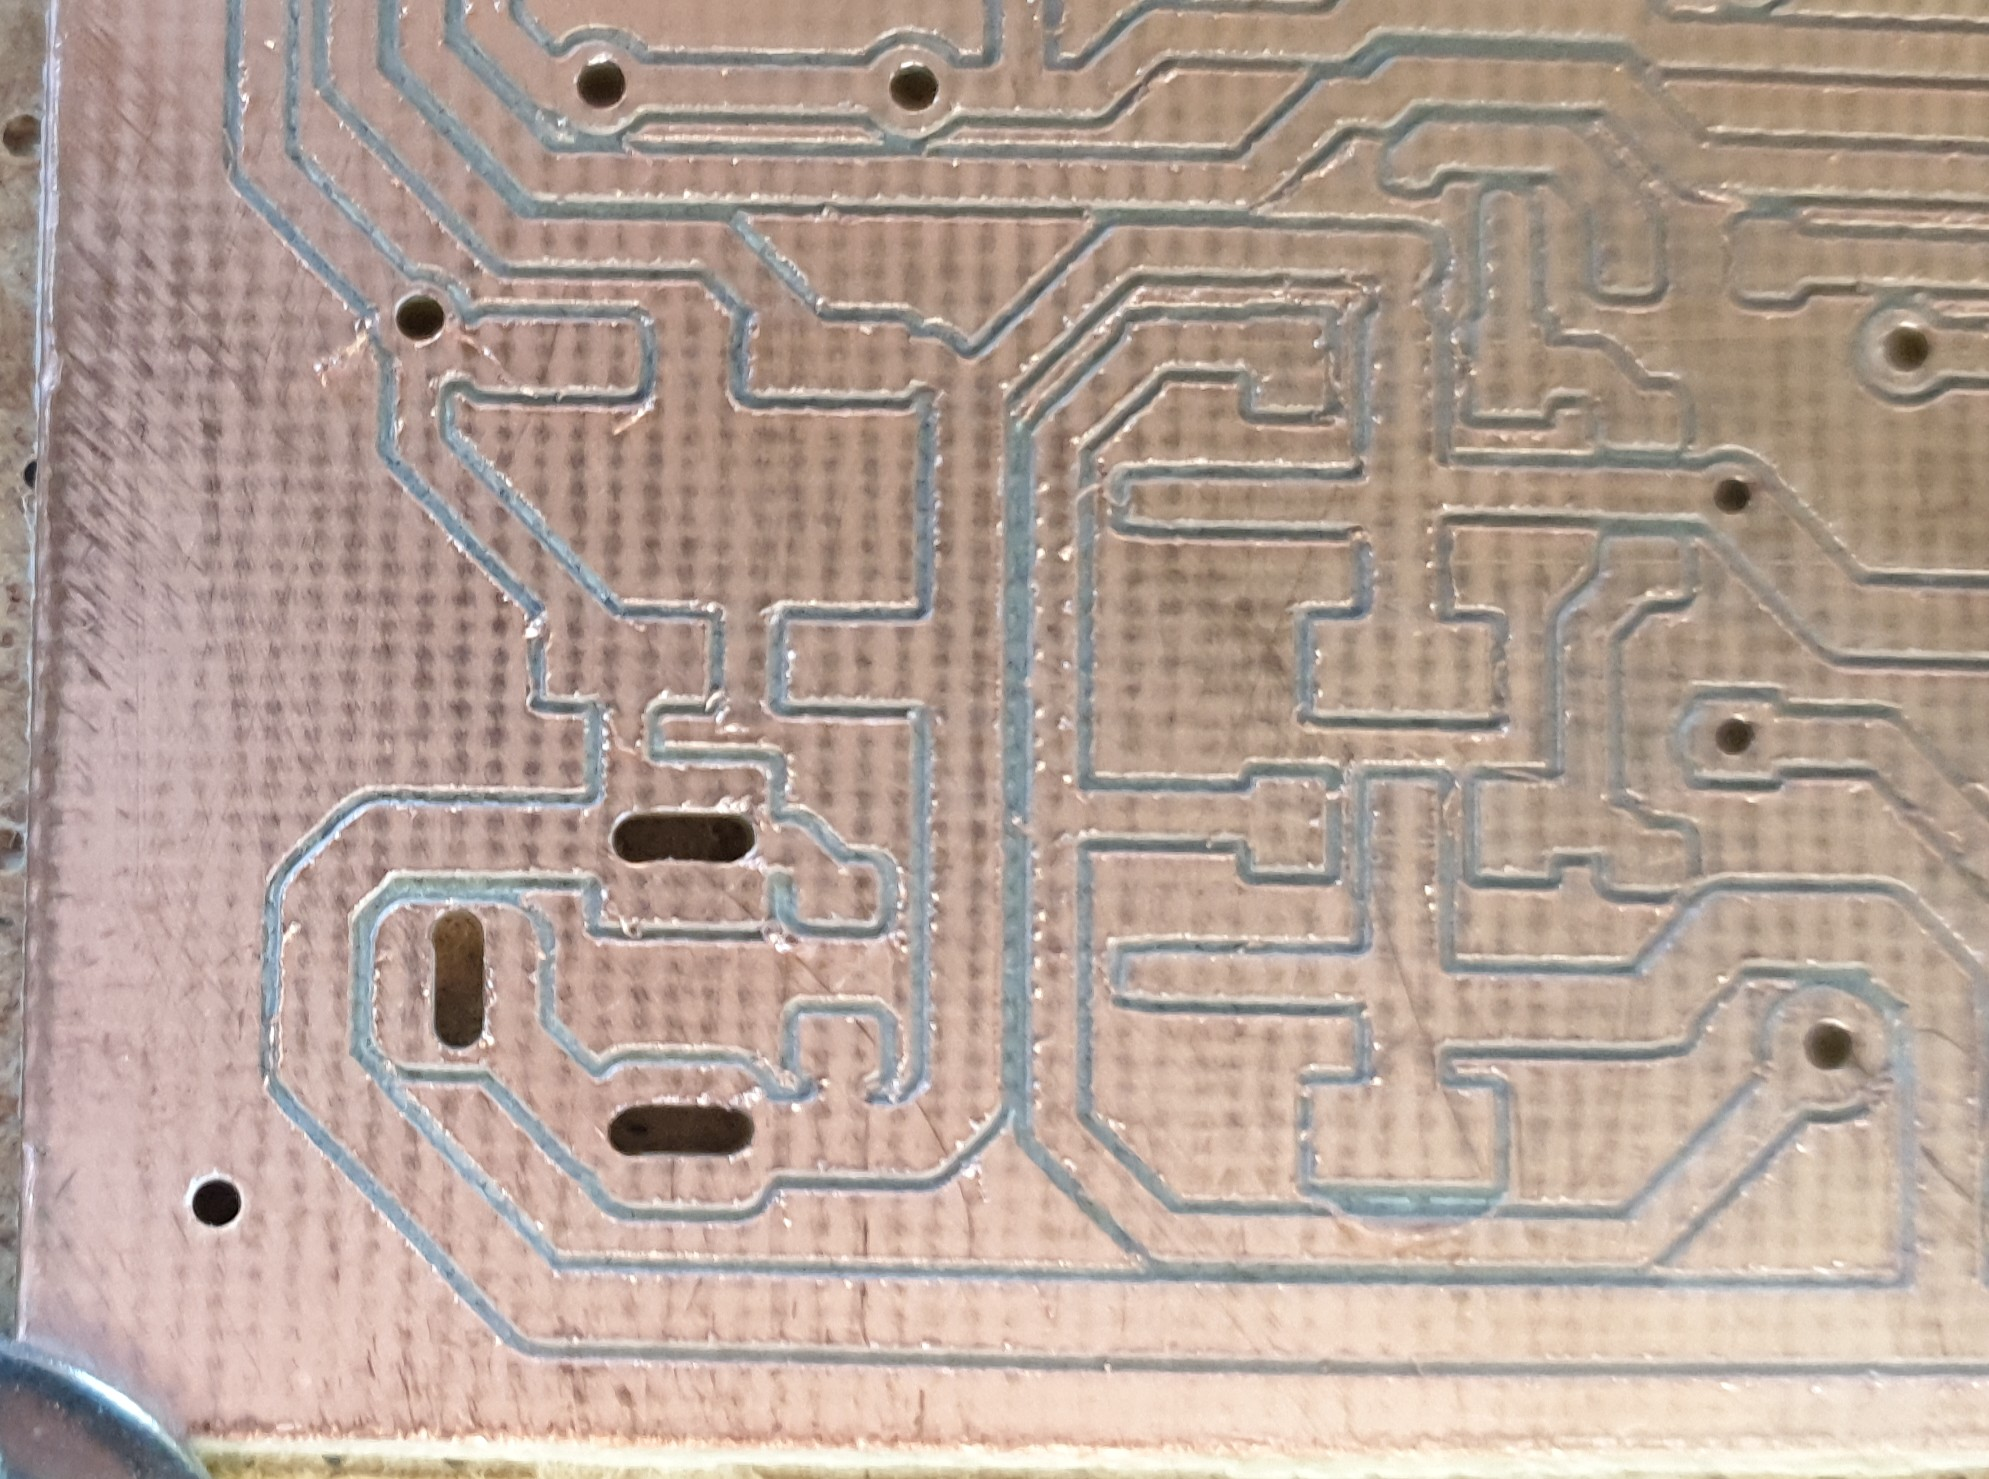
\includegraphics[width=0.25\textwidth]{CNC-drazky}
    \caption{Frézování drážek pro vývody napájecího konektoru}
    \label{fig:CNC drazky}
\end{figure}

\begin{figure}[htbp]
    \centering
    \includegraphics[width=0.80\textwidth]{CNC-outline}
    \caption{Frézování okraje DPS}
    \label{fig:CNC outline}
\end{figure}


\paragraph{Řídicí software}
Řízení vlastního stroje (krokových motorů a vřetena) je řešeno mikrokontrolérem
na jeho desce s řídicí elektronikou. Jeho firmware Grbl implementuje jazyk
G-kód, příkazy jsou přijímány na sériovém portu. Tyto příkazy by bylo možné
zasílat z běžného terminálu, pro zvýšení pohodlí při obsluze stroje je ale
vhodné využít specializovaný software. Jedním z takových programů je
Candle\footnote{\url{https://github.com/Denvi/Candle}}. Jde o svobodný software
distribuovaný pod licencí GNU GPL v3.0. Kromě GNU/Linux je podporován
i operační systém Microsoft Windows. Uživatelské rozhraní tohoto programu (viz
obrázek~\vref{fig:CNC Candle} velmi dobře funguje s dotykovým monitorem.
Jednoduché operace je možné provádět přímo dedikovanými tlačítky či klávesovými
zkratkami, složitější příkazy je možné vypisovat přímo do okna \uv{Console}.

% Stabilní verze z větve \gitbranch{master} je již poměrně stará, proto je
% využívána vývojová verze z větve \gitbranch{Experimental}.
% https://github.com/Denvi/Candle/issues/488#issuecomment-858985048

\begin{figure}[htbp]
    \centering
    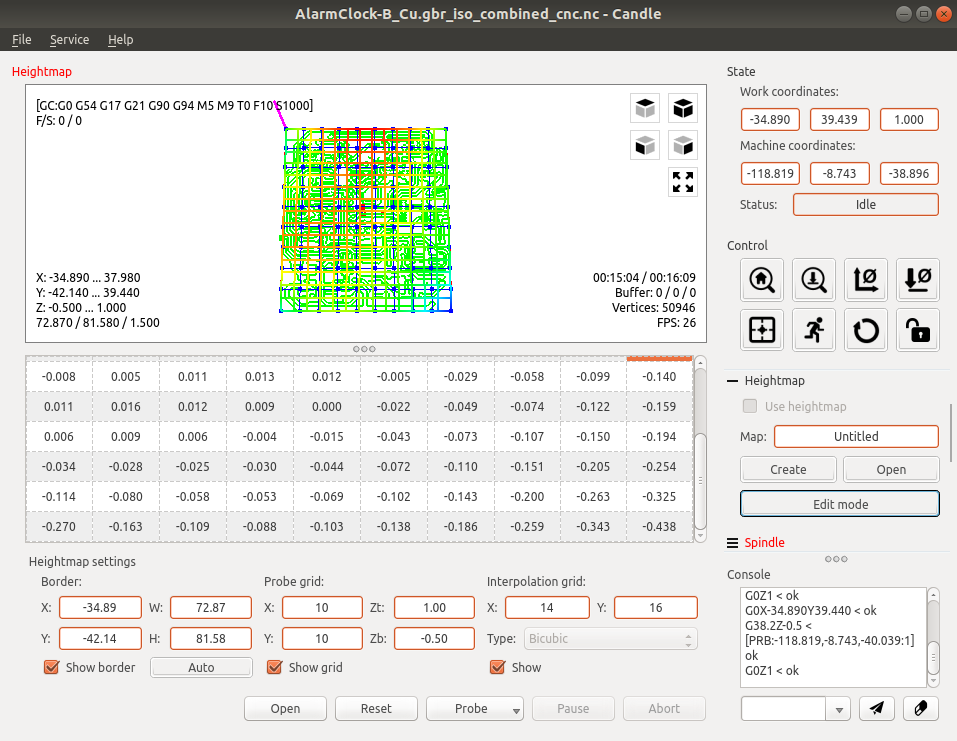
\includegraphics[width=\textwidth]{Candle-UI}
    \caption{Uživatelské rozhraní programu Candle}
    \label{fig:CNC Candle}
\end{figure}


\subsubsection{Generování G-kódu}
G-kód lze psát ručně pomocí běžného textového editoru. Mnohdy je to dokonce
nejrychlejší metoda. Jednoduché operace, jako například vyříznutí hotové DPS
z větší cuprextitové destičky, obvykle sestávají z méně než 15 příkazů
a operátor se základní znalostí G-kódu je zvládne vytvořit velmi rychle.
Složitější operace, jako například frézování vlastního obrazce DPS, ale
vyžadují desítky tisíc příkazů a jejich ruční tvorba by byla prakticky nemožná.
Existuje ale svobodný software FlatCAM\footnote{\url{http://flatcam.org/}},
který slouží k automatickému generování G-kódu z podkladů ve formátu Gerber.
\todo{FlatCAM}


\subsection{Osazování DPS}
Pro osazování součástek pro povrchovou montáž na DPS vyrobenou procesem
frézování nelze využít pájení horkým vzduchem po aplikaci pájecí pasty, protože
by pravděpodobně došlo k nechtěnému připájení součástek k neodfrézované ploše
mědi. Všechny součástky jsou proto pájeny ručně.

\begin{figure}[htb]
    \centering
    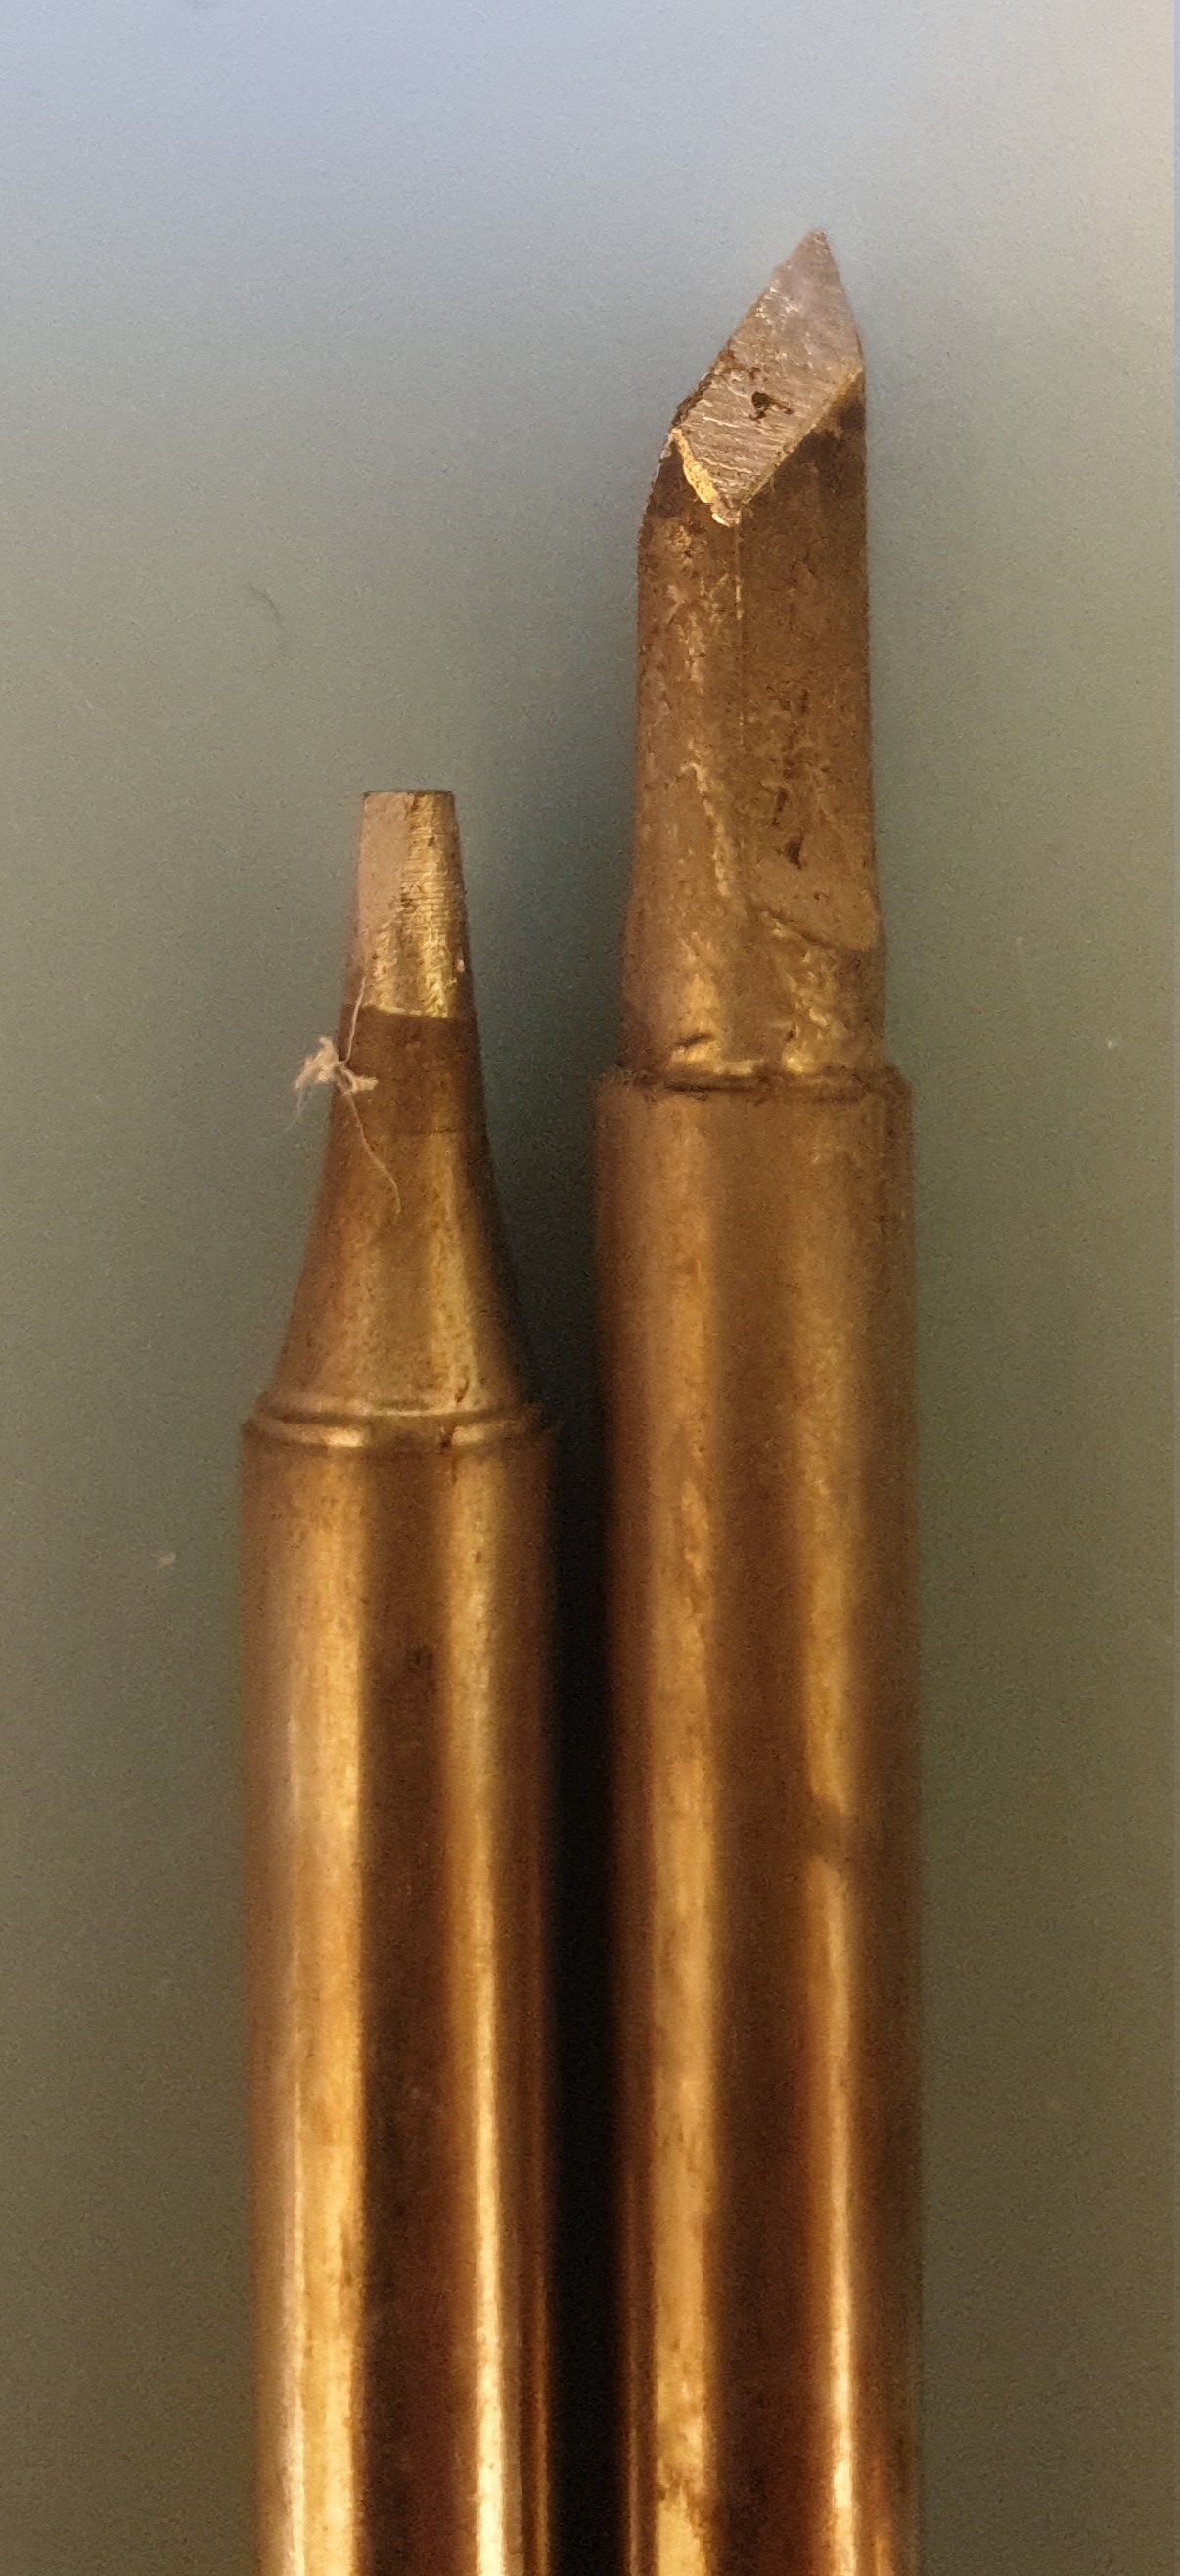
\includegraphics[width=0.45\textwidth,height=60mm,keepaspectratio]{T12-hroty-detail}
    \\
    {\footnotesize Nalevo T12-D16 používaný pro pájení SMD součástek;
    napravo T12-K používaný pro pájení THT součástek.}
    \caption{Hroty pro pájecí stanici T12 používané při osazování DPS}
    \label{fig:PCB pajecka hroty}
\end{figure}

Nejprve osazujeme součástky pro povrchovou montáž (SMT) na spodní straně DPS.
Abychom zabránili poškození polovodičových součástek elektrostatickými výboji,
provádíme osazování a pájení na antistatické podložce. Technik pracující na DPS
by měl nosit antistatický náramek. Je také vhodné nejdříve osazovat pasivní
součástky, aby se riziko poškození polovodičových součástek dále zmenšilo.

Součástky pro THT montáž osazujeme od nejnižších po nejvyšší. Na místo
mikrokontroléru (U2) je vhodné připájet patici, do které se integrovaný obvod
vloží. Pokud byl plošný spoj vyroben jako jednostranný, je nutné vyrobit
a připájet několik drátových propojek.

Při osazování je výhodné využít interaktivní osazovací plán, který je generován
pluginem do KiCAD zvaným
\texttt{InteractiveHtmlBom}\footnote{\url{https://github.com/openscopeproject/InteractiveHtmlBom}}.
Pro jeho zobrazení je využit webový prohlížeč, ve kterém se otevře soubor
\repopath{AlarmClock/bom/ibom.html} z repozitáře \gitrepo{AlarmClock-hardware}.

\begin{figure}[htbp]
    \centering
    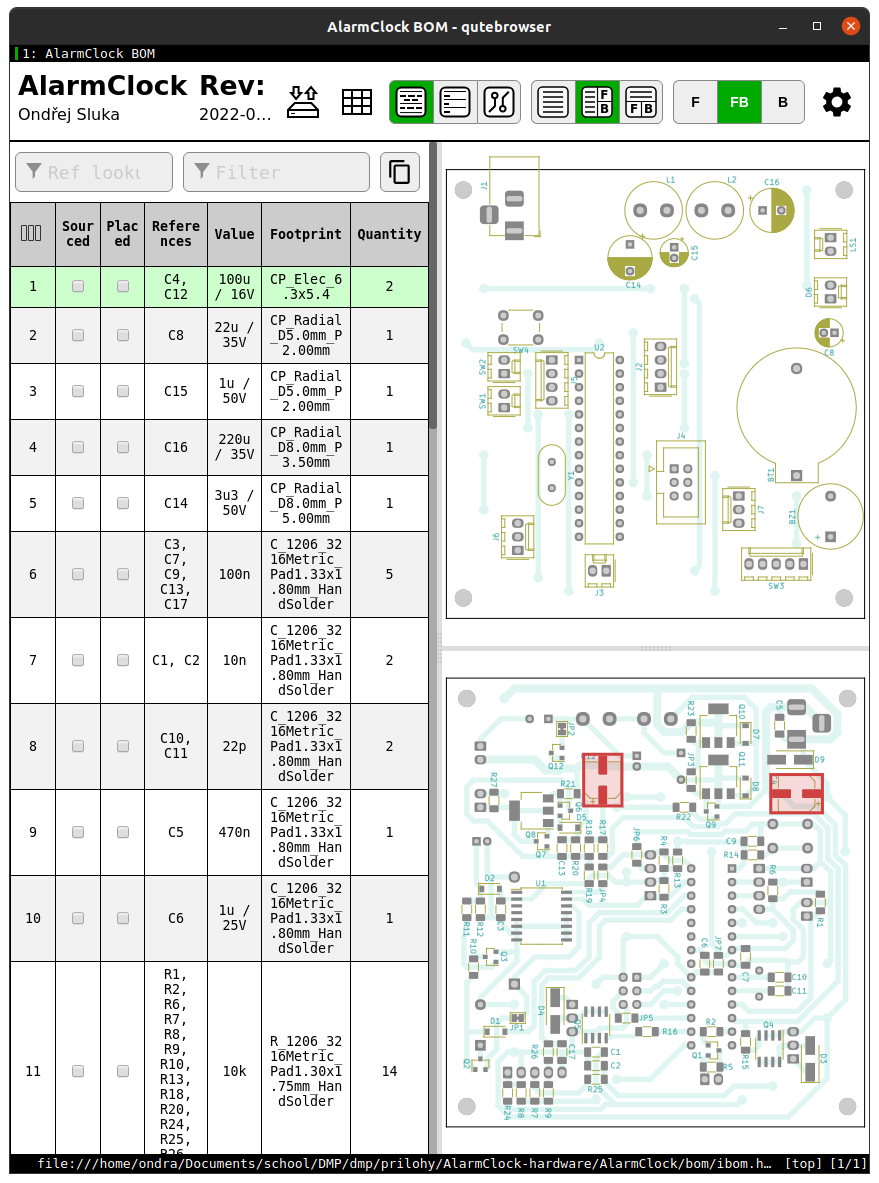
\includegraphics[width=\textwidth]{KICAD-ibom}
    \caption{Interaktivní osazovací plán}
    \label{fig:PCB ibom}
\end{figure}


\subsubsection{Modifikace LCD modulu}
Modul s I/O expandérem PCF8574 je nutné před připájením na zadní stranu LCD
upravit. Obsahuje totiž pull-up rezistory na sběrnici \IIC{}, které by po jeho
připojení tvořili paralelní kombinaci s rezistory na hlavní DPS. Modul také
obsahuje červenou SMD LED, která po připojení napájení neustále svítí.
\todo[inline]{modifikace LCD modulu (odpajeni 3 odporu)}


\subsection{Oživování DPS}
Prvotní testy funkčnosti DPS lze provádět před vložením MCU do patice. Záložní
baterii RTC je vhodné vyjmout z držáku, abychom zabránili jejímu vybití častým
spínáním bzučáku~-- ten totiž při zapnutí DPS bez MCU či s MCU bez validního
firmware nepřetržitě píská. Na jednotlivé piny patice můžeme přivádět různé
signály či provádět měření napětí na nich pomocí digitálního multimetru nebo
osciloskopu. Tímto způsobem lze testovat stmívač LED, zvukový výstup, bzučák
indikující ztrátu napájení a tlačítka. Toto ověření funkčnosti není nutné
provádět, je to ale vhodné pro snížení rizika poškození MCU.

Po provedení základních testů vložíme MCU do patice. Nahrání firmware se
provádí pomocí ISP programátoru USBasp připojeného ke konektoru J4. Postup
programování je popsán v souboru \repopath{README.md} repozitáře
\gitrepo{AlarmClock}. Po nahrání firmware by měla DPS být plně funkční, není
nutné provádět žádná další analogová nastavení.

\chapter{Software}
\todo[inline]{Uvod - cemu rikam software a cemu firmware}
\section{PyAlarmClock}
Pro usnadnění manipulace s budíkem připojeným přes rozhraní UART z počítače
byla vytvořena knihovna \texttt{PyAlarmClock}. Je to modul jazyka Python
obsahující abstrakce pro práci s budíkem. Programátor vytvářející počítačový
program díky tomu nemusí ani znát konkrétní příkazy prostředí
\texttt{AlarmClockCLI}. Například nastavení data času modulu RTC se provádí
přiřazením objektu \texttt{datetime.datetime} vlastnosti \verb|RTC_time|
objektu \texttt{AlarmClock} bez nutnosti znát vnitřní implementaci, která
využívá příkazu \texttt{st} pro nastavení času a \texttt{sd} pro nastavení
data.

Pro ilustraci konceptu poslouží jeden z ukázkových programů~--
\repopath{examples/set_time.py}. V následující ukázce je navíc odstraněna část
zapínající podrobné protokolování všech událostí.
\begin{lstlisting}[language=Python,style=numbers]
#!/usr/bin/env python3

import PyAlarmClock
from datetime import datetime
import time

with PyAlarmClock.SerialAlarmClock('/dev/ttyUSB0') as ac:
    ac.RTC_time = datetime.now()
    time.sleep(1.65)  # RTC is polled every 0.8 seconds
    print(ac.RTC_time)
\end{lstlisting}
Program naváže spojení s budíkem, nastaví čas uložený v RTC na aktuální čas,
počká \SI{1,65}{\second} (aby stihl firmware budíku přečíst novou hodnotu
z RTC) a vypíše do konzole čas přečtený z budíku.
\begin{lstlisting}[style=terminal]
$ ./set_time.py
2022-02-08 19:21:48
$
\end{lstlisting}


\subsection{MQTT adaptér}
Jedním z programů využívajících knihovnu \texttt{PyAlarmClock} je
\repopath{examples/mqtt_bridge.py}. Tento program umožňuje vzdálené ovládání
budíku zprávami přenášenými protokolem MQTT. Tímto způsobem lze zajistit
ovládání budíku několika programy současně bez nutnosti sdílet sériový port
mezi více procesy. Komunikace může probíhat nejen mezi více zařízeními ve
stejné počítačové síti, ale i v rámci jednoho serveru (\texttt{localhost}).

Použití adaptéru je velmi jednoduché. Příkazem \verb|mqtt_bridge.py --help|
lze vypsat seznam argumentů, které lze programu předávat.
% nechci sem davat cely usage, protoze bych ho pak treba musel aktualizovat...
Následuje jednoduchý příklad~-- program se připojí k MQTT brokeru na
\texttt{localhost} na výchozím portu 1883 jako uživatel \texttt{DEBUG} s heslem
zadaným interaktivně za běhu programu:
\begin{lstlisting}[style=terminal]
$ ./examples/mqtt_bridge.py /dev/ttyUSB0 -u DEBUG
Password:
2022-02-08 19:22:39,360 INFO err topic: alarmclock/err
2022-02-08 19:22:39,360 INFO state topic: alarmclock/stat
2022-02-08 19:22:39,360 INFO command topic: alarmclock/cmnd
2022-02-08 19:22:39,361 INFO Connecting to MQTT on localhost:1883
2022-02-08 19:22:42,139 INFO MQTT connected with result code 0

\end{lstlisting}

Pomocí nástrojů ze softwarového balíčku \texttt{mosquitto-clients}
% https://packages.ubuntu.com/focal/mosquitto-clients
můžeme pozorovat, že program při spuštění odešle několik zpráv:
\begin{lstlisting}[style=terminal]
$ mosquitto_sub -v -t alarmclock/#
alarmclock/stat/available online
alarmclock/stat/number_of_alarms 6
\end{lstlisting}
Číslo posílané v topic \topic{alarmclock/stat/number_of_alarms} udává počet
konfigurovatelných časů buzení, které firmware připojeného budíku podporuje
(interně zjišťováno příkazem \texttt{ver}). Zpráva je adaptérem zasílána
s příznakem \texttt{retain}, proto je automaticky zaslána nově příchozímu
subscriberovi.

Zpráva v topic \topic{alarmclock/stat/available} určuje, zda je adaptér
aktivní. Při jeho ukončení či náhodném odpojení je MQTT brokerem do tohoto
topic automaticky zaslána zpráva \texttt{offline}. K tomu je využívána funkce
MQTT \ac{LWT}.

Požadujeme-li, aby budík provedl nějakou akci, pošleme zprávu do příslušného
\texttt{command topic} -- \topic{alarmclock/cmnd/nazev_prikazu}.
Toto je interně řešeno pomocí základních tříd \texttt{AlarmClockMQTT.Entity}
a \texttt{AlarmClockMQTT.Command}, ze kterých dědí třídy reprezentující
jednotlivé komponenty budíku. \texttt{Entity} reprezentuje komponentu mající
nějaký stav, který je možné na vyžádání přečíst
(\foreignlanguage{english}{polling}). \texttt{Command} reprezentuje příkaz,
který je možné spustit MQTT zprávou. Příkazy nemají žádný vlastní stav.
Třídy jednotlivých komponent mohou dědit z obou těchto tříd zároveň~--
například \texttt{Switch} je přepínač, který lze vzdáleně ovládat a jehož stav
je možné i číst.

\begin{lstlisting}[language=Python]
class AlarmClockMQTT:
    """An MQTT adapter for AlarmClock."""

    class Entity:
        """Representation of an AlarmClock attribute with a pollable state."""

        def get_state(self, ac: AlarmClock):
            """Get state of the entity.

            Returns a result that should be published in the entity's
            state_topic.
            """
            raise NotImplementedError()

    class CommandError(Exception):
        """Error raised by a MQTT command handler."""

    class Command:
        """Representation of a MQTT command handler."""

        def do_command(self, ac: AlarmClock, msg: str):
            """Handle reception of msg.

            The return value (if not None) of this function will be published
            in the corresponding state_topic.

            If a tuple is returned, the first value in the tuple is a topic
            under state_topic where the second value should be published.

            If a list is returned, each item will be handled according to
            the above rules.
            """
            raise NotImplementedError()
\end{lstlisting}

Instance \texttt{AlarmClockMQTT} má svá asociativní pole
\texttt{ENTITIES} a \texttt{COMMANDS}, ve kterých jsou uloženy jednotlivé
instance entit a příkazů přiřazené ke svému \texttt{topic}.

\begin{lstlisting}[language=Python]
class AlarmClockMQTT:
    # ...

    def __init__(self, config: AlarmClockMQTTConfig):
        # ...
        ambient = self.DimmableLight('ambient')

        self.COMMANDS: Dict[str, AlarmClockMQTT.Command] = {
            'ambient': ambient,
            # ...
        }

        self.ENTITIES: Dict[str, AlarmClockMQTT.Entity] = {
            'ambient': ambient,
            # ...
        }
\end{lstlisting}

Pro všechny entity, které nejsou zároveň příkazem, je implementováno čtení na
vyžádání, které se provádí MQTT zprávou se znakem \texttt{?} v \texttt{payload}
zaslanou do \texttt{topic} \topic{alarmclock/cmnd/nazev_entity}. Odpověď je
zaslána do \topic{alarmclock/stat/nazev_entity}, \texttt{payload} zprávy je
určen konkrétní implementací metody \verb|get_state| v objektu dané entity.
Entity, které jsou zároveň příkazem (nebo čisté příkazy bez vlastního stavu),
musí zprávy s \lstinline[language=Python]{payload = '?'} v případě potřeby
ošetřit ve vlastní implementaci metody \verb|do_command|. Do
\topic{alarmclock/stat/nazev_entity} je poté zaslána hodnota vrácená touto
metodou. Informace o případných chybách jsou zasílány do
\topic{alarmclock/err}.

\begin{lstlisting}[language=Python]
class AlarmClockMQTT:
    # ...

    def _on_message(self, client, userdata, msg):
        if self._config.command_topic in msg.topic:
            command_id = remove_prefix(msg.topic,
                                       f'{self._config.command_topic}/')
            payload = msg.payload.decode('ascii')
            if command_id in self.COMMANDS:
                self._execute_command(client, command_id, payload)
            elif command_id in self.ENTITIES and payload == '?':
                entity_id = command_id
                self._report_state(client, entity_id)
            else:
                text = f'Bad topic for command: {msg.topic}'
                _LOGGER.error(text)
                client.publish(self._config.err_topic, text)

    def _report_state(self, client: mqtt.Client, entity_id: str):
        client.publish(f'{self._config.state_topic}/{entity_id}',
                       self.ENTITIES[entity_id].get_state(self.ac))

    def _execute_command(self, client: mqtt.Client, command_name: str,
                         msg: str):
        try:
            ret = self.COMMANDS[command_name].do_command(self.ac, msg)
            if ret is not None:
                if not isinstance(ret, list):
                    ret = [ret]
                for value in ret:
                    if isinstance(value, tuple):
                        topic, message = value
                        client.publish(f'{self._config.state_topic}/{topic}',
                                       message)
                    else:
                        client.publish(
                                f'{self._config.state_topic}/{command_name}',
                                value
                                )
        except self.CommandError as e:
            # ...
\end{lstlisting}

V následujícím příkladu je demonstrované rozsvícení připojeného světla
\texttt{lamp} vzdáleným MQTT příkazem a následné zhasnutí pomocí rozhraní na
displeji budíku. Pro přehlednost byly přidány prázdné řádky. První zpráva
v druhém bloku je příkaz pro rozsvícení lampy. V odpověď na ni přichází zpráva
v topic \topic{alarmclock/stat/lamp} značící, že byla lampa rozsvícena. Protože
firmware budíku podporuje funkci přidanou z vývojové větve
\texttt{feature/CLI-BEL}, posílá při každé změně stavu hardware na sériový port
netisknutelný ASCII znak BEL (\texttt{0x07}). V reakci na to si adaptér vyžádá
stav všech hardwarových výstupů a odešle příslušné MQTT zprávy. Zpráva o stavu
lampy je proto duplikována, je ale zajištěna zpětná kompatibilita s firmware
bez podpory funkce asynchronní detekce změn stavu hardware.
Díky této funkci je detekováno i vypnutí lampy přímo ovládacími prvky budíku,
které vede k odeslání třetího bloku zpráv.
\begin{lstlisting}[style=terminal]
$ mosquitto_sub -v -t alarmclock/#
alarmclock/stat/available online
alarmclock/stat/number_of_alarms 6

alarmclock/cmnd/lamp ON
alarmclock/stat/lamp ON
alarmclock/stat/lamp ON
alarmclock/stat/inhibit OFF
alarmclock/stat/ambient 0

alarmclock/stat/lamp OFF
alarmclock/stat/inhibit OFF
alarmclock/stat/ambient 0
\end{lstlisting}

\todo[inline]{dopsat mqtt bridge}

\section{AlarmClockWeb}
Nastavení budicích časů z~rozhraní na LCD budíku je poměrně pohodlné
a~přímočaré, pokud ale uživatel potřebuje udělat rozsáhlejší úpravy, může
preferovat konfiguraci z~počítače či mobilního telefonu.
Z~tohoto důvodu byla vytvořena jednoduchá webová stránka sloužící k~tomuto
účelu. Stránka je tvořena skriptem v~jazyce PHP, který se připojí na MQTT API
budíku a~z~dat z~něj získaných vygeneruje obsah webové stránky ve značkovacím
jazyce HTML. Tato stránka obsahuje formulář, jehož odesláním je možné provádět
v~nastavení budíku změny. Data z~formuláře jsou PHP skriptem parsována
a~následně serializována do JSON objektu kompatibilního s~API budíku.


\begin{figure}[htbp]
    \centering
    \tikzstyle{box}=[draw, rounded corners=2mm, font={\bfseries}, align=center, inner sep=3mm]
    \begin{tikzpicture}[>=latex]
        \node [box] (httpd) at (0,0) {Apache\\\shellcmd{httpd}};
        \node [box] (browser) at (-4.5,0) {Webový\\prohlížeč};
        \draw [<->] (httpd) -- (browser)
            node [midway,above] {\footnotesize HTTP}
            node [midway,below] {\footnotesize HTML}
            ;
        \node [box] (php) at (0,-2) {PHP};
        \draw [<->] (httpd) -- (php);
        \node [align=center, font={\bfseries}] (mqtt_adapter label) at (0,-5) {MQTT\\adaptér};
        \node [box, below=of mqtt_adapter label] (PyAlarmClock) {PyAlarmClock};
        \node [box, fit={(mqtt_adapter label) (PyAlarmClock)}] (mqtt_adapter) {};
        \draw [<->] (mqtt_adapter) -- (php)
            node [midway,sloped,above] {\footnotesize MQTT}
            node [midway,sloped,below] {\footnotesize JSON}
            ;
        \node [box] (AlarmClock) at (6,0 |- PyAlarmClock.east) {Budík\\ATmega328P};
        \draw [<->] (PyAlarmClock) -- (AlarmClock)
            node [midway,sloped,above] {\footnotesize UART}
            node [midway,sloped,below] {\footnotesize YAML}
            ;
        \node [draw, dashed, inner sep=2mm, fit={(httpd) (php)}] (AlarmClockWeb) {}
            node[above, font={\bfseries}] at (AlarmClockWeb.north) {AlarmClockWeb};
    \end{tikzpicture}

    {\footnotesize Nad šipkou je uveden komunikační protokol, pod šipkou je
    formát přenášených dat.}
    \caption{Diagram ilustrující integraci AlarmClockWeb se zbytkem systému}
    \label{fig:web blok}
\end{figure}


\begin{figure}[htbp]
    \centering
    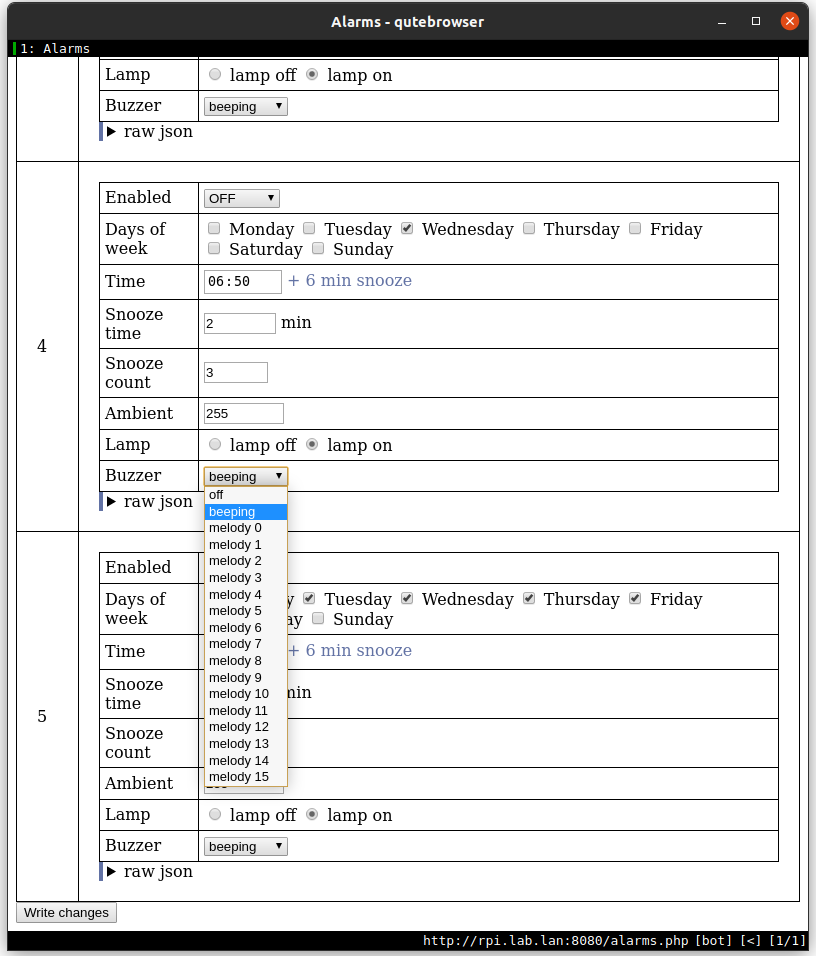
\includegraphics[width=1.00\textwidth]{web-qutebrowser}
    \caption{%
        Webová stránka AlarmClockWeb zobrazená ve webovém prohlížeči
        \shellcmd{qutebrowser}
    }
    \label{fig:web qutebrowser}
\end{figure}

Webová stránka je z~hlediska využitých technologií velice jednoduchá, například
vůbec nevyžaduje JavaScript pro základní funkčnost (JavaScript je ale využíván
pro některé doplňkové funkce). Z~tohoto důvodu by měla být kompatibilní
s~naprostou většinou webových prohlížečů, včetně zastaralých verzí či textových
prohlížečů pro příkazový řádek (viz obrázek~\vref{fig:web links}).

\begin{figure}[htbp]
    \begin{lstlisting}[style=terminal,columns=fixed]
                                                    Alarms (p1 of 13) 
     * home                                                           
     * alarms                                                         
                                                                      
                                Alarms                                
                                                                      
   This simple UI allows for reading and writing configuration of     
   alarms.                                                            
                                                                      
   +--------------------------------------------------------------+   
   | Index | Configuration                                        |   
   |-------+------------------------------------------------------|   
   |       | +--------------------------------------------------+ |   
   |       | | Enabled      | [OFF____]                         | |   
   |       | |--------------+-----------------------------------| |   
   |       | |              | [ ] Monday [ ] Tuesday [ ]        | |   
   |       | | Days of week | Wednesday [ ] Thursday [X] Friday | |   
   |       | |              | [ ] Saturday [ ] Sunday           | |   
   |       | |--------------+-----------------------------------| |   
   |       | | Time         | 12:34________________             | |   
   |       | |--------------+-----------------------------------| |   
   |       | | Snooze time  | 1____________________  min        | |   
   |       | |--------------+-----------------------------------| |   
Select field, name a0-enabled                                        
    \end{lstlisting}
    {\footnotesize (Menu \uv{Enabled} je rozbalené. Ve skutečném terminálu je
    vybraná položka zvýrazněna prohozením barvy pozadí a~popředí.)}
    \caption{AlarmClockWeb v~terminálovém webovém prohlížeči \shellcmd{links}}
    \label{fig:web links}
\end{figure}

Použitá knihovna \texttt{php-mqtt/client} vyžaduje PHP verze 7.4. Operační
systém Debian 10 (buster) ale nabízí ve standardních repozitářích pouze PHP
7.3. Existuje možnost doinstalovat balíčky třetích stran, to by ale mohlo
způsobit problémy s~ostatními službami běžícími na stejném systému (pokud
potřebují PHP 7.3 a~s~PHP 7.4 nefungují).
U~programů napsaných v~jazyce Python (jako například MQTT adaptér) je řešení
podobných problémů velice jednoduché, protože můžeme využít virtuální prostředí
\texttt{virtualenv}. Pro PHP spouštěné webových serverem Apache ale žádné
podobné jednoduché řešení neexistuje.
Proto byl vytvořen soubor \filename{Dockerfile}, který obsahuje definici
kontejneru. V~tomto kontejneru běží zcela oddělená instance Apache s~vlastní
konfigurací a~vlastní verzí PHP. To přináší i~další výhody. Protože služba běží
ve velice dobře definovaném prostředí, které je na všech systémech stejné,
snižuje se například riziko výskytu chyb vyplývajících z~konfigurace
webserveru. Jako základ je použit kontejner \texttt{php:7.4-apache}, do kterého
je doinstalován program pro instalaci PHP knihoven \shellcmd{composer}
a~nakopírovány zdrojové kódy AlarmClockWeb.
\lstinputlisting[language=Dockerfile,style=numbers]{prilohy/AlarmClockWeb/Dockerfile}
Pořadí příkazů v~\filename{Dockerfile} je důležité. Nejde jen o~běžné požadavky
(například soubor musí být do kontejneru nakopírován před tím, než jej můžeme
číst). Každá instrukce \texttt{RUN}, \texttt{COPY} či \texttt{ADD} vytváří
novou vrstvu. Jednotlivé vrstvy jsou drženy v~mezipaměti a~drobná změna ve
zdrojových kódech naší webové aplikaci proto nemusí nutně znamenat sestavení
celého obrazu od úplného počátku. Z~tohoto důvodu je vhodné sestavit
\filename{Dockerfile} tak, aby změna v~jednom ze zdrojových souborů aplikace
nevedla k~invalidaci celé mezipaměti. Tato změna totiž vyžaduje pouze
nakopírování nového souboru do obrazu kontejneru, není ale třeba například
znovu instalovat všechny softwarové balíčky.

\shellcmd{docker} umožňuje distribuci již sestavených obrazů, například na
webovém portálu Docker Hub. Pro tento malý projekt s~minimem uživatelů ale
udržování vlastní binární distribuce a~řešení potenciálních bezpečnostních
problémů s~tím spojených není výhodné.


Nasazení služby AlarmClockWeb na linuxový server se zjednodušuje na několik
příkazů:
\begin{lstlisting}[language=mybash,style=numbers]
# Zkopírujeme ukázkovou konfiguraci do config.php
cp config-sample.php config.php
# Nyní je potřeba konfiguraci upravit a správně nastavit
# např. adresu MQTT brokeru.

# Sestavíme obraz kontejneru z instrukcí v Dockerfile.
docker build -t alarmclockweb .

# Spustíme vlastní kontejner.
# Soubor config.php v aktuální složce ($PWD) je připojen
# ke kontejneru.
# Pokud již na portu 80 poslouchá jiná služba,
# můžeme použít například -p 8080:80.
docker run -d \
    --name alarmclockweb \
    -p 80:80 \
    -v $PWD/config.php:/var/www/html/config.php:ro \
    alarmclockweb
\end{lstlisting}

Pokud je požadována integrace se složitější webovou stránkou, lze v~konfiguraci
jejího webového serveru nastavit funkci reverzní proxy. Tímto způsobem lze
i~přidat dodatečné funkce, jako například ověřování uživatelských hesel.
Následuje příklad konfigurace webového serveru Apache.
Předpokladem je, že kontejner \texttt{alarmclockweb} vystavuje port
\port{8080}. Pro zamezení přímého připojení uživatele na port \port{8080}
serveru je vhodné specifikovat při spouštění kontejneru argument
\texttt{-p 127.0.0.1:8080:80}, kterým je připojení na port \port{8080} omezeno
na rozhraní \texttt{loopback} s~IP adresou \ipaddress{127.0.0.1}.
\begin{lstlisting}[language=hashcomment]
# alarmclockweb docker container
<Location /alarmclock>
    ProxyHTMLEnable On
    ProxyHTMLURLMap / /alarmclock/
    RequestHeader unset Accept-Encoding
    ProxyHTMLCharsetOut *
    AuthType Basic
    AuthName "AlarmClockWeb"
    AuthBasicProvider file
    # htpasswd -c /etc/apache2/.htpasswd ondra
    # (-c means create/rewrite)
    AuthUserFile /etc/apache2/.htpasswd
    Require user ondra
</Location>
ProxyPass /alarmclock http://localhost:8080/
ProxyPassReverse /alarmclock http://localhost:8080/
\end{lstlisting}

\section{Home Assistant}
\todo[inline]{info o HA}

% https://www.home-assistant.io/docs/glossary/

% jinja2 templates

\todo[inline]{verze HA, se kterou pracuji}

MQTT adaptér \shellcmd{mqtt_bridge.py} popisovaný v předchozím textu
umožňuje snadnou integraci s tímto systémem. Platforma \texttt{mqtt} nabízí
v prostředí Home Assistant možnost vytvářet entity z celé řady domén~--
například \HAdomain{sensor}, \HAdomain{binary_sensor}, \HAdomain{light},
\HAdomain{switch} a další.

Příkladem funkce budíku, kterou lze do tohoto systému snadno integrovat, je
ovládání světla \uv{lamp}. To je určeno primárně pro buzení, není ale důvod,
proč by nemohlo být využíváno i pro jiné účely. Protože jde o osvětlení,
využijeme typ entity
\href{https://www.home-assistant.io/integrations/light.mqtt}{MQTT Light}.
Vlastní konfigurace je triviální:
\begin{lstlisting}[language=yaml]
light:
  - platform: mqtt
    name: AlarmClock lamp
    state_topic: alarmclock/stat/lamp
    command_topic: alarmclock/cmnd/lamp
    availability_topic: alarmclock/stat/available
\end{lstlisting}
Využíváme totiž výchozích hodnot -- například \lstinline!payload_off: OFF!
a~\lstinline!payload_on: ON!. Ty se shodují se zprávami odesílanými programem
\shellcmd{mqtt_bridge.py}. \yamlkey{availability_topic} složí k detekci
nefunkčního spojení s budíkem. V takovém případě přejde entita
\HAentity{light.alarmclock_lamp} do stavu \HAstate{unavailable}.

Platforma \foreignlanguage{english}{MQTT Light} umožňuje i ovládání jasu
světla, čehož využíváme u stmívatelného LED pásku \uv{ambient}. Konfigurace je
o něco složitější.
\begin{lstlisting}[language=yaml]
light:
  - platform: mqtt
    schema: template
    name: AlarmClock ambient
    availability_topic: alarmclock/stat/available
    command_topic: alarmclock/cmnd/ambient
    state_topic: alarmclock/stat/ambient
    state_template: "{{ 'off' if value == '0' else 'on' }}"
    brightness_template: "{{ value }}"
    command_off_template: 0
    command_on_template: >
      
      {{ brightness }}
      
      255
      
\end{lstlisting}
Protože je LED pásek řízen pouze jasem, kde hodnota \num{255} představuje plný
jas a \num{0} představuje zhasnuté světlo, je stav entity (zapnuto / vypnuto)
z tohoto čísla. To je úlohou šablony \yamlkey{state_template}. Protože proměnná
\texttt{value} představuje textový řetězec přijatý na \yamlkey{state_topic},
porovnáváme ji s textovým řetězcem \lstinline[language=Python]!'0'!. Druhou
možností by bylo převést \texttt{value} na celočíselný datový typ filtrem
\texttt{int} a porovnávat čísla.

\yamlkey{brightness_template} určuje, jak z přijaté MQTT zprávy odvodit jas
světla jako číslo v rozsahu \numrange{0}{255}.

\yamlkey{command_off_template} určuje zprávu, která se má poslat na
\yamlkey{command_topic}, když je požadováno vypnutí světla. Protože vypnutí
provádíme nastavením jasu na \num{0}, není ani potřeba využít šablonu.

\yamlkey{command_on_template} je složitější, protože musí správně reagovat
v různých situacích:
\begin{enumerate}[nosep]
    \item Je požadováno zapnutí světla, ale není specifikován jas. V takovém
        případě není proměnná \texttt{brightness} definována a do
        \yamlkey{command_topic} se pošle hodnota \num{255}.
    \item Je požadované zapnutí světla s určitou hodnotou jasu. V takovém
        případě se v~MQTT zprávě pošle hodnota proměnné \texttt{brightness}.
\end{enumerate}

\begin{figure}[htb]
    \centering
    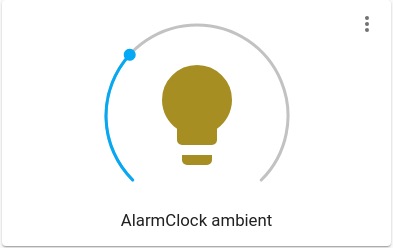
\includegraphics[width=0.3\textwidth]{homeassistant-lovelace-light}
    \caption{%
        Karta \href{https://www.home-assistant.io/lovelace/light/}{Light}
        reprezentující entitu \HAentity{light.alarmclock_ambient} v prostředí
        Lovelace systému Home Assistant
    }
    \label{fig:homeassistant lovelace light}
\end{figure}


\todo[inline]{repozitar s HA konfiguraci}

\subsection{MQTT ping}  % TODO
\todo[inline]{tohle uz je outdated, bylo to nespravnym nastavenim ACL}
Kvůli chybě ve firmwaru jiného zařízení nesouvisejícího s tímto projektem
bylo odhaleno, že když dojde k zahlcení MQTT brokeru Mosquitto zprávami, dojde
k jeho selhání selhání. Zaseknutý broker nenahlásí žádné chyby, neukončí se,
takže ho \shellcmd{systemd} nemůže automaticky restartovat, nebrání klientům
v připojení, ale přestane doručovat zprávy.

Řešením problému byla oprava chyby ve firmware zmíněného zařízení. Abych
v budoucnu zabránil podobným problémům, které by mohly ovlivnit i tento
projekt, vytvořil jsem v systému Home Assistant automatizaci monitorující stav
MQTT brokeru. Automatizace zašle v případě problémů s MQTT brokerem e-mailovou
notifikaci.

Relevantní části souboru \texttt{configuration.yaml}:
\begin{lstlisting}[language=yaml]
recorder:
  # ...
  exclude:
    entities:
      - sensor.last_mqtt_ping
      # MQTT ping automation often updates last_triggered
      - automation.mqtt_ping_2
      # ...


template:
  - trigger:
      # update the sensor every minute
      - platform: time_pattern
        seconds: 3
    binary_sensor:
      - name: MQTT broker
        device_class: connectivity
        state: >-
          {{
          states("sensor.last_mqtt_ping") != "unknown" and
          as_timestamp(now()) - as_timestamp(states("sensor.last_mqtt_ping")) < 620
          }}


sensor:
  - platform: mqtt
    name: Last MQTT ping
    state_topic: mqttping


notify:
  - platform: smtp
    name: email example
    sender: homeassistant@example.com
    # recipient is only used when the service is called without a `target`
    recipient: user@example.com
    server: smtp.example.com
    port: 465
    encryption: tls
    username: !secret smtp_username
    password: !secret smtp_password

  - platform: group
    name: MQTT ping failed
    services:
      - service: email_example
        data:
          target: user@example.com
      - service: persistent_notification
\end{lstlisting}


Vlastní automatizace:
\begin{lstlisting}[language=yaml, style=numbers]
- id: '1629722205484'
  alias: MQTT ping
  description: Periodically send test message to the MQTT broker.
  trigger:
    - platform: time_pattern
      minutes: /10
    - platform: homeassistant
      event: start
    - platform: state
      entity_id: sensor.last_mqtt_ping
      to: unknown
  condition: []
  action:
    - service: mqtt.publish
      data:
        topic: mqttping
        payload_template: '{{now()}}'
  mode: single

- id: '1629722456228'
  alias: MQTT broken
  description: Notify if the MQTT broker is broken.
  trigger:
    - platform: state
      entity_id: binary_sensor.mqtt_broker
      to: 'off'
      for:
        hours: 0
        minutes: 1
        seconds: 5
  condition: []
  action:
    - service: notify.mqtt_ping_failed
      data:
        title: MQTT broker is broken
        message: |-
          MQTT pings are failing.
          Time: {{now()}}
          states("sensor.last_mqtt_ping"): {{states("sensor.last_mqtt_ping")}}
  mode: single
\end{lstlisting}


Související nastavení ACL brokeru Mosquitto:
\begin{lstlisting}
user hass
topic readwrite mqttping
\end{lstlisting}


První automatizace každých 10 minut posílá aktuální čas ve formátu ISO8601 na
topic \topic{mqttping}. Senzor \HAentity{sensor.last_mqtt_ping} zachycuje
zprávy na tomto topicu a jeho stav je shodný s payloadem přijaté zprávy.
Senzor \HAentity{binary_sensor.mqtt_broker} každou minutu ověřuje, jestli je
stav senzoru \HAentity{sensor.last_mqtt_ping} parsovaný jako čas déle starší
než \SI{620}{\second}. Pokud ano, nabývá binární senzor hodnoty \HAstate{off}.
V opačném případě nabývá hodnoty \HAstate{on}.

Druhá automatizace se spustí, pokud je stav senzoru
\HAentity{binary_sensor.mqtt_broker} \HAstate{off} déle než \SI{10}{\second},
a rozešle notifikace o zaseknutí brokeru.



% Reference a odkazy
{\singlespacing%
\printbibliography[title={Odkazy a~literatura}]
\todo[inline]{poznamky a odkazy ??}
\phantomsection
\addcontentsline{toc}{chapter}{Odkazy a~literatura}  % v toc, ale bez cisla
\todo{abecedni razeni seznamu literatury}
}

\listoffigures
\phantomsection
\addcontentsline{toc}{chapter}{\listfigurename}  % v toc, ale bez cisla

\listoftables
\phantomsection
\addcontentsline{toc}{chapter}{\listtablename}  % v toc, ale bez cisla


\nonuchapter{Seznam zkratek}
% POZOR podle abecedy to musim radit rucne...
% vim select in visual mode & :sort
\begin{acronym}[EEPROM] % nejdelsi zkratka kvuli zarovnani
    \acro{CI}{průběžná integrace\acroextra{ (\foreignlanguage{english}{continuous integration})}}
    \acro{CLI}{příkazový řádek\acroextra{ (\foreignlanguage{english}{command line interface})}}
    \acro{CNC}{počítačové číslicové řízení\acroextra{ (\foreignlanguage{english}{computer numeric control})}}
    \acro{DPS}{deska plošných spojů}
    \acro{DRC}{nástroj pro kontrolu návrhu DPS\acroextra{ (\foreignlanguage{english}{Design Rules Checker})}}
    \acro{EEPROM}{elektricky vymazatelná paměť pouze pro čtení\acroextra{ (\foreignlanguage{english}{electrically erasable programmable read-only memory})}}
    \acro{ERC}{nástroj pro kontrolu elektrických pravidel\acroextra{ (\foreignlanguage{english}{Electrical Rules Checker})}}
    \acro{IDE}{vývojové prostředí\acroextra{ (\foreignlanguage{english}{integrated development environment})}}
    \acro{ISP}{\foreignlanguage{english}{in-system programming}}
    \acro{ISR}{obsluha přerušení\acroextra{ (\foreignlanguage{english}{interrupt service routine})}}
    \acro{LED}{elektroluminiscenční dioda\acroextra{ (\foreignlanguage{english}{light-emitting diode})}}
    \acro{LSB}{nejméně významný bit\acroextra{ (\foreignlanguage{english}{least significant bit})}}
    \acro{LUT}{vyhledávací tabulka\acroextra{ (\foreignlanguage{english}{lookup table})}}
    \acro{LWT}{\foreignlanguage{english}{Last Will and Testament}\acroextra{ (funkce protokolu MQTT)}}
    \acro{MCU}{mikrokontrolér\acroextra{ (jednočipový počítač; \foreignlanguage{english}{microcontroller unit})}}
    \acro{MSB}{nejvýznamnější bit\acroextra{ (\foreignlanguage{english}{most significant bit})}}
    \acro{PWM}{pulzně šířková modulace\acroextra{ (\foreignlanguage{english}{pulse-width modulation})}}
    \acro{RTC}{hodiny reálného času\acroextra{ (\foreignlanguage{english}{real-time clock})}}
    \acro{SDK}{software development kit}
    \acro{SMD}{součástka pro povrchovou montáž\acroextra{ (\foreignlanguage{english}{surface mount device})}}
    \acro{SRAM}{statická polovodičová pamět s~přímým přístupem\acroextra{ (\foreignlanguage{english}{static random-access memory})}}
    % TODO \acro{MQTT}{} ??
    % TODO \acro{UART}{} ??
    % TODO \acro{CC}{} ?? constant current
    % TODO \acro{CV}{} ?? constant voltage
\end{acronym}



\listoftodos


\listofappendices
\addcontentsline{toc}{chapter}{\listappendicesname}

\appendix
\pagenumbering{Roman}

\newappendix{Získávání snímků obrazovky z~digitálního osciloskopu Agilent~54621A}
Autorův digitální osciloskop Agilent~54621A má poškozenou disketovou mechaniku,
proto není možné využít standardní metody získávání snímků obrazovky
a~textových dat. Pro účely tvorby dokumentace pro tuto práci byl vyvinut
jednoduchý počítačový program umožňující čtení obrázků ve formátu BMP přes
sériový port RS-232.

Je potřeba použít RS-232 kabel zapojený podle diagramu v dokumentaci
osciloskopu.

\begin{figure}[htbp]
    \centering
    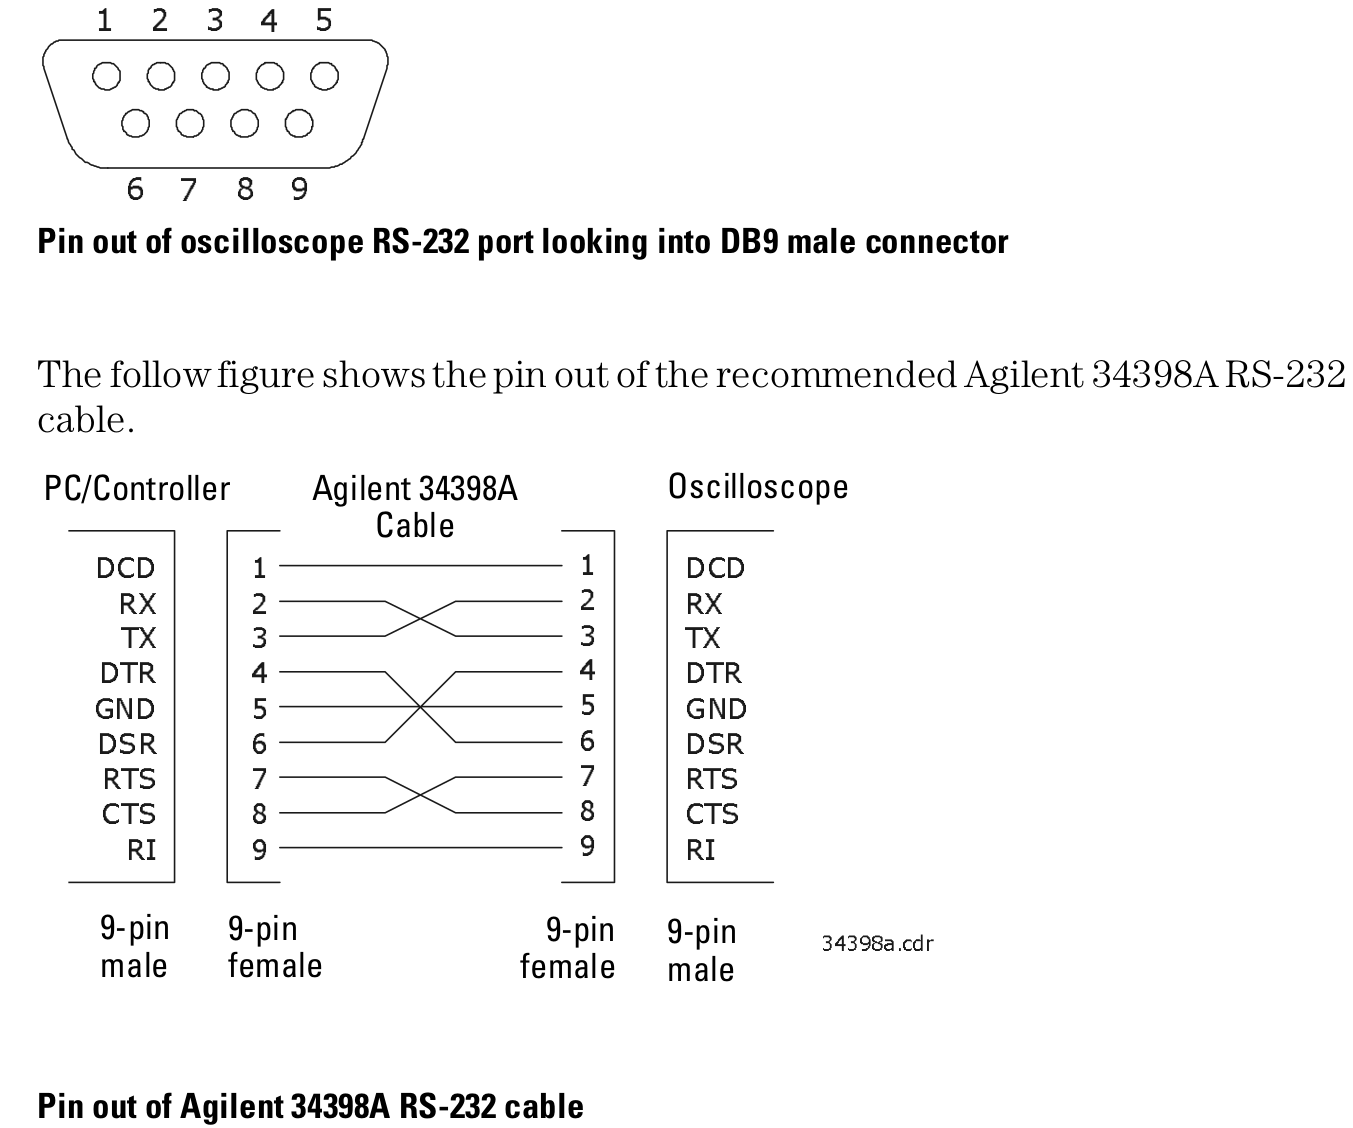
\includegraphics[width=\textwidth]{Agilent-RS232-pinout}
    \caption{%
        Zapojení kabelu pro propojení osciloskopu Agilent~54621A
        s~počítačem~\cite{Agilent54621Auser}
    }
    \label{fig:agilent RS232 pinout}
\end{figure}

Program napsaný v jazyce Python je uložen v souboru \filename{scrot}:
\lstinputlisting[language=Python,style=numbers]{prilohy/scrot}

Příklad použití v prostředí operačního systému GNU/Linux:
\begin{lstlisting}[style=terminal]
$ ./scrot -h
usage: scrot [-h] device file

positional arguments:
  device      Serial port the scope is attached to
  file        File to write the output to

optional arguments:
  -h, --help  show this help message and exit

$ ./scrot /dev/ttyUSB1 nazev-souboru
Screen image written to nazev-souboru.bmp
$
\end{lstlisting}


% TODO prilohy
% mozna dirtree https://www.ctan.org/pkg/dirtree
% TODO zdrojaky LTspice simulaci ??


\end{document}
